\documentclass{manual}
\usepackage{palatino}
\renewcommand{\ttdefault}{cmtt}
\renewcommand{\sfdefault}{cmss}
\newcommand{\myhdl}{\protect \mbox{MyHDL}}
\usepackage{graphicx}

\title{The \myhdl\ manual}

\author{Jan Decaluwe}
\authoraddress{
Email: \email{jan@jandecaluwe.com}
}

\date{May 1, 2006}    	% XXX update before release!
\release{0.5.1}  	        % software release, not documentation
\setreleaseinfo{}		% empty for final release
\setshortversion{0.5}		% major.minor only for software


\makeindex

\begin{document}

\maketitle

Copyright \copyright{} 2003-2006 Jan Decaluwe.
All rights reserved.


\begin{abstract}

\noindent

The goal of the \myhdl{} project is to empower hardware designers with
the elegance and simplicity of the Python language.

\myhdl{} is a free, open-source (LGPL) package for using Python as a
hardware description and verification language. Python is a very high
level language, and hardware designers can use its full power to model
and simulate their designs. Moreover, \myhdl{} can convert a design to
Verilog. In combination with an external synthesis tool, it provides a
complete path from Python to a silicon implementation.

\emph{Modeling}


Python's power and clarity make \myhdl{} an ideal solution for high level
modeling. Python is famous for enabling elegant solutions to complex
modeling problems. Moreover, Python is outstanding for rapid
application development and experimentation.

The key idea behind \myhdl{} is the use of Python generators to model
hardware concurrency. Generators are best described as resumable
functions. In \myhdl{}, generators are used in a specific way so that
they become similar to always blocks in Verilog or processes in VHDL.

A hardware module is modeled as a function that returns any number of
generators. This approach makes it straightforward to support features
such as arbitrary hierarchy, named port association, arrays of
instances, and conditional instantiation.

Furthermore, \myhdl{} provides classes that implement traditional
hardware description concepts. It provides a signal class to support
communication between generators, a class to support bit oriented
operations, and a class for enumeration types.

\emph{Simulation and Verification}

The built-in simulator runs on top of the Python interpreter. It
supports waveform viewing by tracing signal changes in a VCD file.

With \myhdl{}, the Python unit test framework can be used on hardware
designs. Although unit testing is a popular modern software
verification technique, it is not yet common in the hardware design
world, making it one more area in which \myhdl{} innovates.

\myhdl{} can also be used as hardware verification language for VHDL and
Verilog designs, by co-simulation with traditional HDL simulators.

\emph{Conversion to Verilog}

The converter to Verilog works on an instantiated design that has been
fully elaborated. Consequently, the original design structure can be
arbitrarily complex.

The converter automates certain tasks that are tedious or hard in
Verilog directly. Notable features are the possibility to choose
between various FSM state encodings based on a single attribute, the
mapping of certain high-level objects to RAM and ROM descriptions, and
the automated handling of signed arithmetic issues.



\end{abstract}

\tableofcontents

\chapter{Background information \label{background}}

\section{Prerequisites \label{prerequisites}}

You need a basic understanding of Python to use \myhdl{}.
If you don't know Python, don't worry: it
it is one of the easiest programming languages to
learn~\footnote{You must be bored by such claims, but in Python's
case it's true.}. Learning Python is one of the best time
investments that engineering professionals can make~\footnote{I am not
biased.}.

For starters, \url{http://www.python.org/doc/current/tut/tut.html} is
probably the best choice for an on-line tutorial. For alternatives,
see \url{http://www.python.org/doc/Newbies.html}.

A working knowledge of a hardware description language such as Verilog
or VHDL is helpful. 

Code examples in this manual are sometimes shortened for clarity.
 Complete executable examples can be found in the distribution directory at 
\file{example/manual/}.

\section{A small tutorial on generators \label{tutorial}}
\index{generators!tutorial on}

Generators are a relatively recent Python feature. They
were introduced in Python~2.2.
Because generators are the key concept in
\myhdl{}, a small tutorial is included a here.

Consider the following nonsensical function:

\begin{verbatim}
def function():
    for i in range(5):
        return i
\end{verbatim}

You can see why it doesn't make a lot of sense. As soon as the first
loop iteration is entered, the function returns:

\begin{verbatim}
>>> function()
0
\end{verbatim}

Returning is fatal for the function call. Further loop iterations
never get a chance, and nothing is left over from the function call
when it returns.

To change the function into a generator function, we replace
\keyword{return} with \keyword{yield}:

\begin{verbatim}
def generator():
    for i in range(5):
        yield i
\end{verbatim}

Now we get:

\begin{verbatim}
>>> generator()
<generator object at 0x815d5a8>
\end{verbatim}

When a generator function is called, it returns a generator object. A
generator object supports the iterator protocol, which is an expensive
way of saying that you can let it generate subsequent values by
calling its \function{next()} method:

\begin{verbatim}
>>> g = generator()
>>> g.next()
0
>>> g.next()
1
>>> g.next()
2
>>> g.next()
3
>>> g.next()
4
>>> g.next()
Traceback (most recent call last):
  File "<stdin>", line 1, in ?
StopIteration
\end{verbatim}

Now we can generate the subsequent values from the for loop on demand,
until they are exhausted. What happens is that the
\keyword{yield} statement is like a
\keyword{return}, except that it is non-fatal: the generator remembers
its state and the point in the code when it yielded. A higher order
agent can decide when to get the next value by calling the
generator's \function{next()} method. We say that generators are
\dfn{resumable functions}.

If you are familiar with hardware description languages, this may ring
a bell. In hardware simulations, there is also a higher order agent,
the Simulator, that interacts with such resumable functions; they are
called 
\index{VHDL!process}%
\dfn{processes} in VHDL and 
\index{Verilog!always block}%
\dfn{always blocks} in
Verilog.  Similarly, Python generators provide an elegant
and efficient method to model concurrency, without having to resort to
some form of threading.

The use of generators to model concurrency is the first key concept in
\myhdl{}. The second key concept is a related one: in \myhdl{}, the
yielded values are used to specify the conditions on which the
generator should wait before resuming. In other words, \keyword{yield}
statements work as general 
    \index{sensitivity list}%
sensitivity lists. 

For more info about generators, consult the on-line Python
documentation, e.g. at \url{http://www.python.org/doc/2.2.2/whatsnew}. 


\section{About decorators \label{deco}}
\index{decorators!about}

Python 2.4 introduced a new feature called decorators. MyHDL 0.5 takes
advantage of this new feature by defining a number of decorators that
facilitate hardware descriptions. However, many users may not yet be familiar with
decorators. Therefore, an introduction is included here.

A decorator consists of special syntax in front of a function
declaration. It refers to a decorator function. The decorator function
automatically transforms the declared function into some other
callable object.

A decorator function \function{deco} is used in a decorator statement as follows:

\begin{verbatim}
@deco
def func(arg1, arg2, ...):
    <body>
\end{verbatim}

This code is equivalent to the following:

\begin{verbatim}
def func(arg1, arg2, ...):
    <body>
func = deco(func)
\end{verbatim}

Note that the decorator statement goes directly in front of the
function declaration, and that the function name \function{func} is automatically
reused for the final result.

MyHDL 0.5 uses decorators to create ready-to-simulate generators
from local function definitions. Their functionality
and usage will be described extensively in this manual.

For more info about Python decorators, consult the on-line Python
documentation, e.g. at \url{http://www.python.org/doc/2.4/whatsnew/node6.html}.

\begin{notice}[warning]
Because MyHDL 0.5 uses decorators, it requires Python 2.4 or a
later version.
\end{notice}

\chapter{Introduction to \myhdl\ \label{intro}}

\section{A basic \myhdl\ simulation \label{intro-basic}}

We will introduce \myhdl\ with a classic \code{Hello World} style
example. All example code can be found in the distribution directory
under \file{example/manual/}.  Here are the contents of a \myhdl\
simulation script called \file{hello1.py}:

\begin{verbatim}
from myhdl import Signal, delay, always, now, Simulation

def HelloWorld():

    interval = delay(10)
    
    @always(interval)
    def sayHello():
        print "%s Hello World!" % now()

    return sayHello


inst = HelloWorld()
sim = Simulation(inst)
sim.run(30)
\end{verbatim}

When we run this simulation, we get the following output:

\begin{verbatim}
% python hello1.py
10 Hello World!
20 Hello World!
30 Hello World!
_SuspendSimulation: Simulated 30 timesteps
\end{verbatim}

The first line of the script imports a number of objects from the
\code{myhdl} package. In Python we can only use identifiers that are
literally defined in the source file 
\footnote{The exception is the \samp{from module import *} syntax,
that imports all the symbols from a module. Although this is generally
considered bad practice, it can be tolerated for large modules that
export a lot of symbols. One may argue that
\code{myhdl} falls into that category.}.

Then, we define a function called \function{HelloWorld}. In MyHDL,
classic functions are used to model hardware modules. In particular,
the parameter list is used to define the interface. In this first
example, the interface is empty.

Inside the top level function we declare a local function called
\function{sayHello} that defines the desired behavior. This function
is decorated with an \function{always} decorator that has a delay
   \index{decorator!\function{always}}
object as its parameter.  The meaning is that the function will be
executed whenever the specified delay interval has expired.

Behind the curtains, the \function{always} decorator creates a Python
\emph{generator} and reuses the name of the decorated function for
it. Generators are the fundamental objects in MyHDL, and we will say
much more about them further on.

Finally, the top level function returns the local generator. This is
the simplest case of the basic MyHDL code pattern
to define the contents of a hardware module. We will describe the
general case further on.

In MyHDL, we create an \emph{instance} of a hardware module by calling
the corresponding function. In the example, variable \code{inst} refers
to an instance of \function{HelloWorld}.  To simulate the instance, we
pass it as an argument to a \class{Simulation} object constructor.  We
then run the simulation for the desired amount of timesteps.

\section{Signals, ports, and concurrency \label{intro-conc}}

In the previous section, we simulated a design with a single
generator and no concurrency. On the other hand, real hardware
descriptions are typically massively concurrent.
\myhdl\ supports this by allowing an
arbitrary number of concurrently running generators. 

With concurrency comes the problem of deterministic
communication. Hardware languages use special objects to
support deterministic communication between concurrent code.
In particular, \myhdl\ 
has a \class{Signal} object which is roughly modeled after VHDL
signals.

We will demonstrate signals and concurrency
by extending and modifying our first example. We define two hardware
modules, one that drives a clock signal, and one that is sensitive
to a positive edge on a clock signal:


\begin{verbatim}
from myhdl import Signal, delay, always, now, Simulation


def ClkDriver(clk):

    halfPeriod = delay(10)

    @always(halfPeriod)
    def driveClk():
        clk.next = not clk

    return driveClk


def HelloWorld(clk):
    
    @always(clk.posedge)
    def sayHello():
        print "%s Hello World!" % now()

    return sayHello


clk = Signal(0)
clkdriver_inst = ClkDriver(clk)
hello_inst = HelloWorld(clk)
sim = Simulation(clkdriver_inst, hello_inst)
sim.run(50)
\end{verbatim}

The clock driver function \function{ClkDriver} has a
clock signal as its parameter. This is how a
\emph{port} is modeled in MyHDL. The function
defines a generator
that continuously toggles a clock signal after a certain delay.
A new value of a signal is specified by assigning to its
\code{next} attribute. This is the \myhdl\ equivalent of 
    \index{VHDL!signal assignment}%
the VHDL signal assignment and the 
    \index{Verilog!non-blocking assignment}%
Verilog non-blocking assignment.

The \function{HelloWorld} function is modified from the
first example. It now also takes a clock signal as parameter.
Its generator is made sensitive to a rising
    \index{wait!for a rising edge}%
edge of the clock signal. This is specified by the
\code{posedge} attribute of a signal. The edge
specifier is the argument of the \code{always}
decorator. As a result, the decorated function
will be executed on every rising clock edge.

The \code{clk} signal is constructed with an initial value
\code{0}. When creating an instance of each 
hardware module, the same clock signal is passed as
the argument. The result is that the instances
are now connected through the clock signal.
The \class{Simulation} object is constructed with the
two instances.

When we run the simulation, we get:

\begin{verbatim}
% python hello2.py
10 Hello World!
30 Hello World!
50 Hello World!
_SuspendSimulation: Simulated 50 timesteps
\end{verbatim}


\section{Parameters and hierarchy \label{intro-hier}}

We have seen that MyHDL uses functions to model hardware
modules. We have also seen that ports are modeled by using
signals as parameters. To make designs reusable we will also
want to use other objects as parameters. For example, we can
change the clock generator function to make it more general
and reusable, by making the clock period parameterizable, as
follows:

\begin{verbatim}
from myhdl import Signal, delay, instance, always, now, Simulation

def ClkDriver(clk, period=20):
    
    lowTime = int(period/2)
    highTime = period - lowTime

    @instance
    def driveClk():
        while True:
            yield delay(lowTime)
            clk.next = 1
            yield delay(highTime)
            clk.next = 0

    return driveClk
\end{verbatim}

In addition to the clock signal, the clock
period is a parameter, with a default value of \code{20}.

As the low time of the clock may differ from the high time in case of
an odd period, we cannot use the \function{always} decorator with a
single delay value anymore. Instead, the \function{driveClk} function
is now a generator function with an explicit definition of the desired
behavior. It is decorated with the \function{instance} decorator.
    \index{decorator!\function{instance}}
You can see that \function{driveClk} is a generator function
because it contains \code{yield} statements.

When a generator function is called, it returns a generator object.
This is basically what the \function{instance} decorator does. It
is less sophisticated than the \function{always} decorator,
but it can be used to create a generator from any local generator
function.

The \code{yield} statement is a general Python construct, but MyHDL
uses it in a dedicated way.  In MyHDL, it has a similar meaning as the
wait statement in VHDL: the statement suspends execution of a
generator, and its clauses specify the conditions on which the
generator should wait before resuming. In this case, the generator
waits for a certain delay.

Note that to make sure that the generator runs ``forever'', we wrap its
behavior in a \code{while True} loop.

Similarly, we can define a general \function{Hello} function as follows:

\begin{verbatim}
def Hello(clk, to="World!"):

    @always(clk.posedge)
    def sayHello():
        print "%s Hello %s" % (now(), to)

    return sayHello
\end{verbatim}


We can create any number of instances by calling the functions with
the appropriate parameters. Hierarchy can be modeled by defining the
instances in a higher-level function, and returning them.
This pattern can be repeated for an arbitrary number of
hierarchical levels. Consequently, the general definition
of a \myhdl\ instance is recursive: an instance
   \index{instance!defined}%
is either a sequence of instances, or a generator.

As an example, we will create a higher-level function with
four instances of the lower-level functions, and simulate it:

\begin{verbatim}
def greetings():

    clk1 = Signal(0)
    clk2 = Signal(0)
    
    clkdriver_1 = ClkDriver(clk1) # positional and default association
    clkdriver_2 = ClkDriver(clk=clk2, period=19) # named association 
    hello_1 = Hello(clk=clk1) # named and default association
    hello_2 = Hello(to="MyHDL", clk=clk2) # named association

    return clkdriver_1, clkdriver_2, hello_1, hello_2


inst = greetings()
sim = Simulation(inst)
sim.run(50)
\end{verbatim}

As in standard Python, positional or named parameter association can
be used in instantiations, or a mix of both\footnote{All positional
parameters have to go before any named parameter.}. All these styles
are demonstrated in the example above. Named association can be very
useful if there are a lot of parameters, as the argument order in the
call does not matter in that case.

The simulation produces the following output:

\begin{verbatim}
% python greetings.py
9 Hello MyHDL
10 Hello World!
28 Hello MyHDL
30 Hello World!
47 Hello MyHDL
50 Hello World!
_SuspendSimulation: Simulated 50 timesteps
\end{verbatim}


\begin{notice}[warning]
Some commonly used terminology has different meanings
in Python versus hardware design. Rather than artificially
changing terminology, I think it's best to keep it
and explicitly describing the differences.

A \dfn{module} in Python refers to all source code
in a particular file. A module can be reused by
other modules by importing. In hardware design,
\index{module!in Python versus hardware design}%
a module is  a reusable block of hardware with
a well defined interface. It can be reused in 
another module by \dfn{instantiating} it.

An \dfn{instance} in Python (and other object-oriented
languages) refers to the object created by a
\index{instance!in Python versus hardware design}%
class constructor. In hardware design, an instance
is a particular incarnation of a hardware module.

Normally, the meaning should be clear from
the context. Occasionally, I may qualify terms 
with the words 'hardware' or '\myhdl{}' to 
avoid ambiguity.
\end{notice}


\section{Bit oriented operations \label{intro-bit}}

Hardware design involves dealing with bits and bit-oriented
operations. The standard Python type \class{int} has most of the
desired features, but lacks support for indexing and slicing. For this
reason, \myhdl\ provides the \class{intbv} class. The name was chosen
to suggest an integer with bit vector flavor.

Class \class{intbv} works transparently with other
integer-like types. Like class \class{int}, it provides access to the
underlying two's complement representation for bitwise
operations. In addition, it is a mutable type that provides indexing
and slicing operations, and some additional bit-oriented support such
as concatenation.

\subsection{Bit indexing \label{intro-indexing}}
\index{bit indexing}

As an example, we will consider the design of a Gray encoder. The
following code is a Gray encoder modeled in \myhdl{}:

\begin{verbatim}
from myhdl import Signal, delay, Simulation, always_comb, instance, intbv, bin

def bin2gray(B, G, width):
    """ Gray encoder.

    B -- input intbv signal, binary encoded
    G -- output intbv signal, gray encoded
    width -- bit width
    """
    
    @always_comb
    def logic():
        for i in range(width):
            G.next[i] = B[i+1] ^ B[i]
            
    return logic
\end{verbatim}

This code introduces a few new concepts. The string in triple quotes
at the start of the function is a \dfn{doc string}. This is standard
Python practice for structured documentation of code.

Furthermore, we introduce a third decorator: \function{always_comb}.
    \index{decorator!\function{always_comb}}
It is used with a classic function and specifies that the 
resulting generator should
    \index{wait!for a signal value change}%
wait for a value change on any input signal. This is typically used to
describe 
    \index{combinatorial logic}%
combinatorial logic. The \function{always_comb} decorator
automatically infers which signals are used as inputs.

Finally, the code contains bit indexing operations and an exclusive-or
operator as required for a Gray encoder. By convention, the lsb of an
\class{intbv} object has index~\code{0}.

To verify the Gray encoder, we write a test bench that prints input
and output for all possible input values:

\begin{verbatim}
def testBench(width):
    
    B = Signal(intbv(0))
    G = Signal(intbv(0))
    
    dut = bin2gray(B, G, width)

    @instance
    def stimulus():
        for i in range(2**width):
            B.next = intbv(i)
            yield delay(10)
            print "B: " + bin(B, width) + "| G: " + bin(G, width)

    return dut, stimulus
\end{verbatim}

We use the conversion function \code{bin} to get a binary
string representation of the signal values. This function is exported
by the \code{myhdl} package and supplements the standard Python
\code{hex} and \code{oct} conversion functions.

As a demonstration, we set up a simulation for a small width: 

\begin{verbatim}
sim = Simulation(testBench(width=3))
sim.run()
\end{verbatim}

The simulation produces the following output:

\begin{verbatim}
% python bin2gray.py
B: 000 | G: 000
B: 001 | G: 001
B: 010 | G: 011
B: 011 | G: 010
B: 100 | G: 110
B: 101 | G: 111
B: 110 | G: 101
B: 111 | G: 100
StopSimulation: No more events
\end{verbatim}

\subsection{Bit slicing \label{intro-slicing}}
\index{bit slicing}

For a change, we will use a traditional function as an example to illustrate
slicing.  The following function calculates the HEC byte of an ATM
header.

\begin{verbatim}
from myhdl import intbv, concat

COSET = 0x55

def calculateHec(header):
    """ Return hec for an ATM header, represented as an intbv.

    The hec polynomial is 1 + x + x**2 + x**8.
    """
    hec = intbv(0)
    for bit in header[32:]:
        hec[8:] = concat(hec[7:2],
                         bit ^ hec[1] ^ hec[7],
                         bit ^ hec[0] ^ hec[7],
                         bit ^ hec[7]
                        )
    return hec ^ COSET
\end{verbatim}

The code shows how slicing access and assignment is supported on the
\class{intbv} data type. In accordance with the most common hardware
convention, and unlike standard Python, slicing ranges are
downward. The code also demonstrates concatenation of \class{intbv}
objects.

As in standard Python, the slicing range is half-open: the highest
index bit is not included. Unlike standard Python however, this index
corresponds to the \emph{leftmost} item. Both indices can be omitted
from the slice. If the leftmost index is omitted, the meaning is to
access ``all'' higher order bits.  If the rightmost index is omitted,
it is \code{0} by default.

The half-openness of a slice may seem awkward at first, but it helps
to avoid one-off count issues in practice. For example, the slice
\code{hex[8:]} has exactly \code{8} bits. Likewise, the slice
\code{hex[7:2]} has \code{7-2=5} bits. You can think about it as
follows: for a slice \code{[i:j]}, only bits below index \code{i} are
included, and the bit with index \code{j} is the last bit included.

When an intbv object is sliced, a new intbv object is returned. This
new intbv object is always positive, even when the original object
was negative.


\section{Some remarks on \myhdl\ and Python \label{intro-python}}

To conclude this introductory chapter, it is useful to stress that
\myhdl\ is not a language in itself. The underlying language is Python, 
and \myhdl\ is implemented as a Python package called \code{myhdl}.
Moreover, it is a design goal to keep the \code{myhdl} package as
minimalistic as possible, so that \myhdl\ descriptions are very much
``pure Python''.

To have Python as the underlying language is significant in several
ways:

\begin{itemize}

\item Python is a very powerful high level language. This translates
into high productivity and elegant solutions to complex problems.

\item Python is continuously improved by some very clever 
minds, supported by a large and fast growing user base. Python profits
fully from the open source development model.

\item Python comes with an extensive standard library. Some
functionality is likely to be of direct interest to \myhdl\ users:
examples include string handling, regular expressions, random number
generation, unit test support, operating system interfacing and GUI
development. In addition, there are modules for mathematics, database
connections, networking programming, internet data handling, and so
on.

\item Python has a powerful C extension model. All built-in types are
written with the same C API that is available for custom
extensions. To a module user, there is no difference between a
standard Python module and a C extension module --- except
performance. The typical Python development model is to prototype
everything in Python until the application is stable, and (only) then
rewrite performance critical modules in C if necessary.

\end{itemize}


\section{Summary and perspective \label{intro-summary}}
Here is an overview of what we have learned in this chapter:

\begin{itemize}
\item Generators are the basic building blocks of MyHDL models. They
provide the way to model massive concurrency and sensitiviy lists.

\item MyHDL provides decorators that create useful generators from local functions.

\item Hardware structure and hierarchy is described with classic Python functions. 

\item \code{Signal} objects are used to communicate between concurrent generators.

\item \code{intbv} objects are used to describe bit-oriented operations.

\item A \code{Simulation} object is used to simulate MyHDL models.
\end{itemize}

These concepts are sufficient to start describing and simulating MyHDL models.

However, there is much more to MyHDL. Here is an overview of what can
be learned from the following chapters:

\begin{itemize}
\item MyHDL supports sophisticated and high level modeling techniques.
This is described in Chapter~\ref{model}

\item MyHDL enables the use of modern software verfication techniques,
such as unit testing, on hardware designs. This is the topic of
Chapter~\ref{unittest}.

\item It is possible to co-simulate MyHDL models with other HDL
languages such as Verilog and VHDL. This is described in
Chapter~\ref{cosim}.

\item Last but not least, MyHDL models can be converted to
Verilog, providing a path to a silicon implementation. This
is the topic of Chapter~\ref{conv}.
\end{itemize}

\chapter{Modeling techniques \label{model}}

\section{Structural modeling \label{model-structure}}
\index{modeling!structural}

Hardware descriptions need to support the concepts of module
instantiation and hierarchy.  In \myhdl{}, an instance is recursively
defined as being either a sequence of instances, or a generator.
Hierarchy is modeled by defining instances in a higher-level
function, and returning them.  The following is a schematic example
of the basic case.

\begin{verbatim}
def top(...):
    ...
    instance_1 = module_1(...)
    instance_2 = module_2(...)
    ...
    instance_n = module_n(...)
    ... 
    return instance_1, instance_2, ... , instance_n
\end{verbatim}

Note that \myhdl\ uses conventional procedural techniques
for modeling structure. This makes it straightforward
to model more complex cases.

\subsection{Conditional instantiation \label{model-conf}}
\index{conditional instantiation}

To model conditional instantiation, we can
select the returned instance under parameter control.
For example:

\begin{verbatim}
SLOW, MEDIUM, FAST = range(3)

def top(..., speed=SLOW):
    ...
    def slowAndSmall():
       ...
    ...
    def fastAndLarge():
       ...
    if speed == SLOW:
        return slowAndSmall()
    elif speed == FAST:
        return fastAndLarge()
    else:
        raise NotImplementedError
\end{verbatim}


\subsection{Arrays of instances \label{model-instarray}}
\index{arrays of instances}

Python lists are easy to create. We can use them
to model arrays of instances. 

Suppose we have a top module that instantiates a
single \code{channel} submodule, as follows:

\begin{verbatim}
def top(...):

    din = Signal(0)
    dout = Signal(0)
    clk = Signal(bool(0))
    reset = Signal(bool(0))

    channel_inst = channel(dout, din, clk, reset)

    return channel_inst 
\end{verbatim}

If we wanted to support an arbitrary number of channels,
we can use lists of signals and a list of instances,
as follows:

\begin{verbatim}
def top(..., n=8):

    din = [Signal(0) for i in range(n)]
    dout = [Signal(0) for in range(n)]
    clk = Signal(bool(0))
    reset = Signal(bool(0))
    channel_inst = [None for i in range(n)]

    for i in range(n):
        channel_inst[i] = channel(dout[i], din[i], clk, reset)

    return channel_inst
\end{verbatim}

\subsection{Inferring the list of instances \label{model-infer-instlist}}

In \myhdl{}, instances have to be returned explicitly by
a top level function. It may be convenient to assemble 
the list of instances automatically. For this purpose,
\myhdl  provides the function \function{instances()}.
Using the first example in this section, it is used as follows:

\begin{verbatim}
from myhdl import instances

def top(...):
    ...
    instance_1 = module_1(...)
    instance_2 = module_2(...)
    ...
    instance_n = module_n(...)
    ...
    return instances()
\end{verbatim}

Function \function{instances()} uses introspection to inspect the type
of the local variables defined by the calling function. All variables
that comply with the definition of an instance are assembled in
a list, and that list is returned.

\section{RTL modeling \label{model-rtl}}
\index{modeling!RTL style}

The present section describes how \myhdl\ supports RTL style modeling
as is typically used for synthesizable models.

\subsection{Combinatorial logic \label{model-comb}}
\index{combinatorial logic}

\subsubsection{Template \label{model-comb-templ}}
 
Combinatorial logic is described with a code pattern as
follows: 

\begin{verbatim}
def top(<parameters>):
    ...
    @always_comb
    def combLogic():
        <functional code>
    ...
    return combLogic, ...
\end{verbatim}

The \function{always_comb} decorator describes
combinatorial logic.
\footnote{The name \function{always_comb} refers to a construct with
similar semantics in SystemVerilog.}.
The decorated function is a local function that specifies what
happens when one of the input signals of the logic changes.  The
\function{always_comb} decorator infers the input signals
automatically. It returns a generator that is sensitive to all inputs,
and that executes the function whenever an input changes.


\subsubsection{Example \label{model-comb-ex}}

The following is an example of a combinatorial multiplexer:

\begin{verbatim}
from myhdl import Signal, Simulation, delay, always_comb

def Mux(z, a, b, sel):

    """ Multiplexer.
    
    z -- mux output
    a, b -- data inputs
    sel -- control input: select a if asserted, otherwise b

    """

    @always_comb
    def muxLogic():
        if sel == 1:
            z.next = a
        else:
            z.next = b

    return muxLogic
\end{verbatim}


To verify it, we will simulate the logic with some random patterns. The
\code{random} module in Python's standard library comes in handy for
such purposes. The function \code{randrange(\var{n})} returns a random
natural integer smaller than \var{n}. It is used in the test bench
code to produce random input values:

\begin{verbatim}
from random import randrange

z, a, b, sel = [Signal(0) for i in range(4)]

mux_1 = Mux(z, a, b, sel)

def test():
    print "z a b sel"
    for i in range(8):
        a.next, b.next, sel.next = randrange(8), randrange(8), randrange(2)
        yield delay(10)
        print "%s %s %s %s" % (z, a, b, sel)

test_1 = test()

sim = Simulation(mux_1, test_1)
sim.run()    
\end{verbatim}

Because of the randomness, the simulation output varies between runs
\footnote{It also possible to have a reproducible random output, by
explicitly providing a seed value. See the documentation of the
\code{random} module.}. One particular run produced the following
output:

\begin{verbatim}
% python mux.py
z a b sel
6 6 1 1
7 7 1 1
7 3 7 0
1 2 1 0
7 7 5 1
4 7 4 0
4 0 4 0
3 3 5 1
StopSimulation: No more events
\end{verbatim}


\subsection{Sequential logic \label{model-seq}}
\index{sequential logic}

\subsubsection{Template \label{model-seq-templ}}
Sequential RTL models are sensitive to a clock edge. In addition, they
may be sensitive to a reset signal. We will describe one of the most
common patterns: a template with a rising clock edge and an
asynchronous reset signal. Other templates are similar.

\begin{verbatim}
def top(<parameters>, clock, ..., reset, ...):
    ...
    @always(clock.posedge, reset.negedge)
    def seqLogic():
        if reset == <active level>:
            <reset code>
        else:
            <functional code>
    ...
    return seqLogic, ...
\end{verbatim}


\subsubsection{Example \label{model-seq-ex}}
The following code is a description of an incrementer with enable, and
an asynchronous reset.

\begin{verbatim}
from random import randrange
from myhdl import *

ACTIVE_LOW, INACTIVE_HIGH = 0, 1

def Inc(count, enable, clock, reset, n):

    """ Incrementer with enable.
    
    count -- output
    enable -- control input, increment when 1
    clock -- clock input
    reset -- asynchronous reset input
    n -- counter max value

    """

    @always(clock.posedge, reset.negedge)
    def incLogic():
        if reset == ACTIVE_LOW:
            count.next = 0
        else:
            if enable:
                count.next = (count + 1) % n

    return incLogic
\end{verbatim}

For the test bench, we will use an independent clock generator, stimulus
generator, and monitor. After applying enough stimulus patterns, we
can raise the \code{StopSimulation} exception to stop the
simulation run. The test bench for a small incrementer and a small
number of patterns is a follows:

\begin{verbatim}
def testbench():
    count, enable, clock, reset = [Signal(intbv(0)) for i in range(4)]

    inc_1 = Inc(count, enable, clock, reset, n=4)

    HALF_PERIOD = delay(10)

    @always(HALF_PERIOD)
    def clockGen():
        clock.next = not clock

    @instance
    def stimulus():
        reset.next = ACTIVE_LOW
        yield clock.negedge
        reset.next = INACTIVE_HIGH
        for i in range(12):
            enable.next = min(1, randrange(3))
            yield clock.negedge
        raise StopSimulation

    @instance
    def monitor():
        print "enable  count"
        yield reset.posedge
        while 1:
            yield clock.posedge
            yield delay(1)
            print "   %s      %s" % (enable, count)

    return clockGen, stimulus, inc_1, monitor


tb = testbench()

def main():
    Simulation(tb).run()
\end{verbatim}

The simulation produces the following output:
\begin{verbatim}
% python inc.py
enable  count
   0      0
   1      1
   0      1
   1      2
   1      3
   1      0
   0      0
   1      1
   0      1
   0      1
   0      1
   1      2
StopSimulation
\end{verbatim}


\subsection{Finite State Machine modeling \label{model-fsm}}
\index{modeling!Finite State Machine}

Finite State Machine (FSM) modeling is very common in RTL
design and therefore deserves special attention.

For code clarity, the state values are typically represented by a set
of identifiers. A standard Python idiom for this purpose is to assign
a range of integers to a tuple of identifiers, like so:

\begin{verbatim}
>>> SEARCH, CONFIRM, SYNC = range(3)
>>> CONFIRM
1
\end{verbatim}

However, this technique has some drawbacks. Though it is clearly
the intention that the identifiers belong together, this information
is lost as soon as they are defined. Also, the identifiers evaluate to
integers, whereas a string representation of the identifiers
would be preferable. To solve these issues, we need an
\emph{enumeration type}.

\myhdl\ supports enumeration types by providing a function
\function{enum()}.  The arguments to \function{enum()} are the string
representations of the identifiers, and its return value is an
enumeration type. The identifiers are available as attributes of the
type. For example:

\begin{verbatim}
>>> from myhdl import enum
>>> t_State = enum('SEARCH', 'CONFIRM', 'SYNC')
>>> t_State
<Enum: SEARCH, CONFIRM, SYNC>
>>> t_State.CONFIRM
CONFIRM
\end{verbatim}

We can use this type to construct a state signal as follows:

\begin{verbatim}
state = Signal(t_State.SEARCH)
\end{verbatim}

As an example, we will use a framing controller FSM.  It is an
imaginary example, but similar control structures are often found in
telecommunication applications. Suppose that we need to find the
Start Of Frame (SOF) position of an incoming frame of bytes.
A sync pattern detector continuously looks for a framing
pattern and indicates it to the FSM with a \code{syncFlag} signal. When
found, the FSM moves from the initial \code{SEARCH} state to the
\code{CONFIRM} state. When the \code{syncFlag}
is confirmed on the expected position, the FSM declares \code{SYNC},
otherwise it falls back to the \code{SEARCH} state.  This FSM can be
coded as follows:

\begin{verbatim}
from myhdl import *

ACTIVE_LOW = 0
FRAME_SIZE = 8
t_State = enum('SEARCH', 'CONFIRM', 'SYNC')

def FramerCtrl(SOF, state, syncFlag, clk, reset_n):
    
    """ Framing control FSM.

    SOF -- start-of-frame output bit
    state -- FramerState output
    syncFlag -- sync pattern found indication input
    clk -- clock input
    reset_n -- active low reset
    
    """
    
    index = Signal(0) # position in frame

    @always(clk.posedge, reset_n.negedge)
    def FSM():
        if reset_n == ACTIVE_LOW:
            SOF.next = 0
            index.next = 0
            state.next = t_State.SEARCH

        else:
            index.next = (index + 1) % FRAME_SIZE
            SOF.next = 0

            if state == t_State.SEARCH:
                index.next = 1
                if syncFlag:
                    state.next = t_State.CONFIRM

            elif state == t_State.CONFIRM:
                if index == 0:
                    if syncFlag:
                        state.next = t_State.SYNC
                    else:
                        state.next = t_State.SEARCH

            elif state == t_State.SYNC:
                if index == 0:
                    if not syncFlag:
                        state.next = t_State.SEARCH
                SOF.next = (index == FRAME_SIZE-1)

            else:
                raise ValueError("Undefined state")

    return FSM
\end{verbatim}

At this point, we will use the example to demonstrate
the \myhdl\ support for 
\index{waveform viewing}%
waveform viewing.
During simulation, signal
changes can be written to a VCD output file.  The VCD file can then be
loaded and viewed in a waveform viewer tool such as \program{gtkwave}.

The user interface of this feature consists of a single function,
\function{traceSignals()}.  To explain how it works, recall that in
\myhdl{}, an instance is created by assigning
the result of a function call to an instance name.
For example:

\begin{verbatim}
tb_fsm = testbench()
\end{verbatim}

To enable VCD tracing, the instance should be created as follows
instead:

\begin{verbatim}
tb_fsm = traceSignals(testbench)
\end{verbatim}

Note that the first argument of
\function{traceSignals()} consists of the uncalled function. By
calling the function under its control, \function{traceSignals()}
gathers information about the hierarchy and the signals to be traced.
In addition to a function argument, \function{traceSignals()} accepts
an arbitrary number of non-keyword and keyword arguments that will be
passed to the function call. 

A small test bench for our framing controller example,
with signal tracing enabled, is shown below:

\begin{verbatim}
def testbench():

    SOF = Signal(bool(0))
    syncFlag = Signal(bool(0))
    clk = Signal(bool(0))
    reset_n = Signal(bool(1))
    state = Signal(t_State.SEARCH)
            
    framectrl = FramerCtrl(SOF, state, syncFlag, clk, reset_n)

    @always(delay(10))
    def clkgen():
        clk.next = not clk

    @instance
    def stimulus():
        for i in range(3):
            yield clk.posedge
        for n in (12, 8, 8, 4):
            syncFlag.next = 1
            yield clk.posedge
            syncFlag.next = 0
            for i in range(n-1):
                yield clk.posedge
        raise StopSimulation
        
    return framectrl, clkgen, stimulus


tb_fsm = traceSignals(testbench)
sim = Simulation(tb_fsm)
sim.run()
\end{verbatim}

When we run the test bench, it generates a VCD file
called \file{testbench.vcd}. When we load this file into
\program{gtkwave}, we can view the waveforms:

\ifpdf
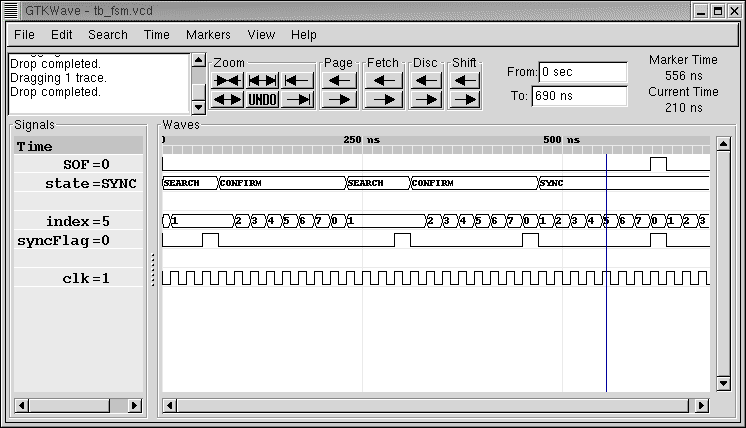
\includegraphics{tbfsm.png}
\fi

Signals are dumped in a suitable format. This format is inferred at
the \class{Signal} construction time, from the type of the initial
value. In particular, \class{bool} signals are dumped as single
bits. (This only works starting with Python~2.3, when \class{bool} has
become a separate type).  Likewise, \class{intbv} signals with a
defined bit width are dumped as bit vectors. To support the general
case, other types of signals are dumped as a string representation, as
returned by the standard \function{str()} function.

\begin{notice}[warning]
Support for literal string representations is not part of the VCD
standard. It is specific to \program{gtkwave}. To generate a
standard VCD file, you need to use signals with a defined bit width
only.
\end{notice}


\section{High level modeling \label{model-hl}}
\index{modeling!high level}

\subsection{Modeling with bus-functional procedures \label{model-bfm}}

\index{bus-functional procedure}%
A \dfn{bus-functional procedure} is a reusable encapsulation of the
low-level operations needed to implement some abstract transaction on
a physical interface. Bus-functional procedures are typically used in
flexible verification environments.

Once again, \myhdl\ uses generator functions to support
bus-functional procedures. In \myhdl\, the difference between
instances and bus-functional procedure calls comes from the way in
which a generator function is used.

As an example, we will design a bus-functional procedure of a
simplified UART transmitter. We assume 8 data bits, no parity bit, and
a single stop bit, and we add print statements to follow the
simulation behavior:

\begin{verbatim}
T_9600 = int(1e9 / 9600)

def rs232_tx(tx, data, duration=T_9600):
    
    """ Simple rs232 transmitter procedure.

    tx -- serial output data
    data -- input data byte to be transmitted
    duration -- transmit bit duration
    
    """

    print "-- Transmitting %s --" % hex(data)
    print "TX: start bit"      
    tx.next = 0
    yield delay(duration)

    for i in range(8):
        print "TX: %s" % data[i]
        tx.next = data[i]
        yield delay(duration)

    print "TX: stop bit"      
    tx.next = 1
    yield delay(duration)
\end{verbatim}

This looks exactly like the generator functions in previous sections. It
becomes a bus-functional procedure when we use it differently. Suppose
that in a test bench, we want to generate a number of data bytes to be
transmitted. This can be modeled as follows:


\begin{verbatim}
testvals = (0xc5, 0x3a, 0x4b)

def stimulus():
    tx = Signal(1)
    for val in testvals:
        txData = intbv(val)
        yield rs232_tx(tx, txData)
\end{verbatim}

We use the bus-functional procedure call as a clause in a
\code{yield} statement. This introduces a fourth form of the
\code{yield} statement: using a generator as a clause. Although this is
a more dynamic usage than in the previous cases, the meaning is
actually very similar: at that point,
the original generator should 
    \index{wait!for the completion of a generator}% 
wait for the completion of a generator. 
In this case, the original generator resumes when the
\code{rs232_tx(tx, txData)} generator returns.

When simulating this, we get:

\begin{verbatim}
-- Transmitting 0xc5 --
TX: start bit
TX: 1
TX: 0
TX: 1
TX: 0
TX: 0
TX: 0
TX: 1
TX: 1
TX: stop bit
-- Transmitting 0x3a --
TX: start bit
TX: 0
TX: 1
TX: 0
TX: 1
...
\end{verbatim}

We will continue with this example by designing the corresponding UART
receiver bus-functional procedure. This will allow us to introduce
further capabilities of \myhdl\ and its use of the \code{yield}
statement. 

Until now, the \code{yield} statements had a single clause. However,
they can have multiple clauses as well. In that case, the generator
resumes as soon as the wait condition specified by one
of the clauses is satisfied. This corresponds to the functionality of
    \index{sensitivity list}%
sensitivity lists in Verilog and VHDL.

For example, suppose we want to design an UART receive procedure with
a timeout. We can specify the timeout condition while waiting for the
start bit, as in the following generator function:

\begin{verbatim}
def rs232_rx(rx, data, duration=T_9600, timeout=MAX_TIMEOUT):
    
    """ Simple rs232 receiver procedure.

    rx -- serial input data
    data -- data received
    duration -- receive bit duration
    
    """

    # wait on start bit until timeout
    yield rx.negedge, delay(timeout)
    if rx == 1:
        raise StopSimulation, "RX time out error"

    # sample in the middle of the bit duration
    yield delay(duration // 2)
    print "RX: start bit"

    for i in range(8):
        yield delay(duration)
        print "RX: %s" % rx
        data[i] = rx

    yield delay(duration)
    print "RX: stop bit"
    print "-- Received %s --" % hex(data)
\end{verbatim}

If the timeout condition is triggered, the receive bit \code{rx}
will still be \code{1}. In that case, we raise an exception to stop
the simulation. The \code{StopSimulation} exception is predefined in
\myhdl\ for such purposes. In the other case, we proceed by
positioning the sample point in the middle of the bit duration, and
sampling the received data bits.

When a \code{yield} statement has multiple clauses, they can be of any
type that is supported as a single clause, including generators. For
example, we can verify the transmitter and receiver generator against
each other by yielding them together, as follows:

\begin{verbatim}
def test():
    tx = Signal(1)
    rx = tx
    rxData = intbv(0)
    for val in testvals:
        txData = intbv(val)
        yield rs232_rx(rx, rxData), rs232_tx(tx, txData)
\end{verbatim}

Both forked generators will run concurrently, and the original
generator will resume as soon as one of them finishes (which will be
the transmitter in this case).  The simulation output shows how
the UART procedures run in lockstep:

\begin{verbatim}
-- Transmitting 0xc5 --
TX: start bit
RX: start bit
TX: 1
RX: 1
TX: 0
RX: 0
TX: 1
RX: 1
TX: 0
RX: 0
TX: 0
RX: 0
TX: 0
RX: 0
TX: 1
RX: 1
TX: 1
RX: 1
TX: stop bit
RX: stop bit
-- Received 0xc5 --
-- Transmitting 0x3a --
TX: start bit
RX: start bit
TX: 0
RX: 0
...
\end{verbatim}

For completeness, we will verify the timeout behavior with a test
bench that disconnects the \code{rx} from the \code{tx} signal, and we
specify a small timeout for the receive procedure:

\begin{verbatim}
def testTimeout():
    tx = Signal(1)
    rx = Signal(1)
    rxData = intbv(0)
    for val in testvals:
        txData = intbv(val)
        yield rs232_rx(rx, rxData, timeout=4*T_9600-1), rs232_tx(tx, txData)
\end{verbatim}
 
The simulation now stops with a timeout exception after a few
transmit cycles:

\begin{verbatim}
-- Transmitting 0xc5 --
TX: start bit
TX: 1
TX: 0
TX: 1
StopSimulation: RX time out error
\end{verbatim}

Recall that the original generator resumes as soon as one of the
forked generators returns. In the previous cases, this is just fine,
as the transmitter and receiver generators run in lockstep. However,
it may be desirable to resume the caller only when \emph{all} of the
forked generators have finished. For example, suppose that we want to
characterize the robustness of the transmitter and receiver design to
bit duration differences. We can adapt our test bench as follows, to
run the transmitter at a faster rate:

\begin{verbatim}
T_10200 = int(1e9 / 10200)

def testNoJoin():
    tx = Signal(1)
    rx = tx
    rxData = intbv(0)
    for val in testvals:
        txData = intbv(val)
        yield rs232_rx(rx, rxData), rs232_tx(tx, txData, duration=T_10200)
\end{verbatim}

Simulating this shows how the transmission of the new byte starts
before the previous one is received, potentially creating additional
transmission errors:

\begin{verbatim}
-- Transmitting 0xc5 --
TX: start bit
RX: start bit
...
TX: 1
RX: 1
TX: 1
TX: stop bit
RX: 1
-- Transmitting 0x3a --
TX: start bit
RX: stop bit
-- Received 0xc5 --
RX: start bit
TX: 0
\end{verbatim}

It is more likely that we want to characterize the design on a byte
by byte basis, and align the two generators before transmitting each
byte. In \myhdl{}, this is done with the \function{join} function. By
joining clauses together in a \code{yield} statement, we create a new
clause that triggers only when all of its clause arguments have
triggered. For example, we can adapt the test bench as follows:

\begin{verbatim}
def testJoin():
    tx = Signal(1)
    rx = tx
    rxData = intbv(0)
    for val in testvals:
        txData = intbv(val)
        yield join(rs232_rx(rx, rxData), rs232_tx(tx, txData, duration=T_10200))
\end{verbatim}

Now, transmission of a new byte only starts when the previous one is received:

\begin{verbatim}
-- Transmitting 0xc5 --
TX: start bit
RX: start bit
...
TX: 1
RX: 1
TX: 1
TX: stop bit
RX: 1
RX: stop bit
-- Received 0xc5 --
-- Transmitting 0x3a --
TX: start bit
RX: start bit
TX: 0
RX: 0
\end{verbatim}



\subsection{Modeling memories with built-in types \label{model-mem}}
\index{modeling!memories}

Python has powerful built-in data types that can be useful to model
hardware memories. This can be merely a matter of putting an interface
around some data type operations.

For example, a \dfn{dictionary} comes in handy to model sparse memory
structures. (In other languages, this data type is called 
\dfn{associative array}, or \dfn{hash table}.) A sparse memory is one in
which only a small part of the addresses is used in a particular
application or simulation. Instead of statically allocating the full
address space, which can be large, it is better to dynamically
allocate the needed storage space. This is exactly what a dictionary
provides. The following is an example of a sparse memory model:

\begin{verbatim}
def sparseMemory(dout, din, addr, we, en, clk):
    
    """ Sparse memory model based on a dictionary.

    Ports:
    dout -- data out
    din -- data in
    addr -- address bus
    we -- write enable: write if 1, read otherwise
    en -- interface enable: enabled if 1
    clk -- clock input
    
    """

    memory = {}

    @always(clk.posedge)
    def access():
        if en:
            if we:
                memory[addr.val] = din.val
            else:
                dout.next = memory[addr.val]

    return access
\end{verbatim} 

Note how we use the \code{val} attribute of the \code{din} signal, as
we don't want to store the signal object itself, but its current
value. Similarly, we use the \code{val} attribute of the \code{addr}
signal as the dictionary key. 

In many cases, \myhdl\ code uses a signal's current value
automatically when there is no ambiguity: for example, when a signal
is used in an expression. However, in other cases such as in this
example you have to refer to the value explicitly: for example, when
the Signal is used as an index, or when it is not used in an
expression.  One option is to use the \code{val} attribute, as in this
example.  Another possibility is to use the \code{int()} or
\code{bool()} functions to typecast the Signal to an integer or a
boolean value. These functions are also useful with \class{intbv}
objects.

As a second example, we will demonstrate how to use a list to model a
synchronous fifo:

\begin{verbatim}
def fifo(dout, din, re, we, empty, full, clk, maxFilling=sys.maxint):
    
    """ Synchronous fifo model based on a list.
    
    Ports:
    dout -- data out
    din -- data in
    re -- read enable
    we -- write enable
    empty -- empty indication flag
    full -- full indication flag
    clk -- clock input

    Optional parameter:
    maxFilling -- maximum fifo filling, "infinite" by default

    """
    
    memory = []

    @always(clk.posedge)
    def access():
        if we:
            memory.insert(0, din.val)
        if re:
            dout.next = memory.pop()
        filling = len(memory)
        empty.next = (filling == 0)
        full.next = (filling == maxFilling)

    return access
\end{verbatim}

Again, the model is merely a \myhdl\ interface around some operations
on a list: \function{insert()} to insert entries, \function{pop()} to
retrieve them, and \function{len()} to get the size of a Python
object.

\subsection{Modeling errors using exceptions \label{model-err}}

In the previous section, we used Python data types for modeling. If
such a type is used inappropriately, Python's run time error system
will come into play. For example, if we access an address in the
\function{sparseMemory} model that was not initialized before, we will
get a traceback similar to the following (some lines omitted for
clarity):

\begin{verbatim}
Traceback (most recent call last):
...
  File "sparseMemory.py", line 31, in access
    dout.next = memory[addr.val]
KeyError: Signal(51)
\end{verbatim}

Similarly, if the \code{fifo} is empty, and we attempt to read from
it, we get:

\begin{verbatim}
Traceback (most recent call last):
...
  File "fifo.py", line 34, in fifo
    dout.next = memory.pop()
IndexError: pop from empty list
\end{verbatim}

Instead of these low level errors, it may be preferable to define
errors at the functional level. In Python, this is typically done by
defining a custom \code{Error} exception, by subclassing the standard
\code{Exception} class. This exception is then raised explicitly when
an error condition occurs.

For example, we can change the \function{sparseMemory} function as
follows (with the doc string is omitted for brevity):

\begin{verbatim}
class Error(Exception):
    pass

def sparseMemory2(dout, din, addr, we, en, clk):
   
    memory = {}

    @always(clk.posedge)
    def access():
        if en:
            if we:
                memory[addr.val] = din.val
            else:
                try:
                    dout.next = memory[addr.val]
                except KeyError:
                    raise Error, "Uninitialized address %s" % hex(addr)

    return access

\end{verbatim}

This works by catching the low level data type exception, and raising
the custom exception with an appropriate error message instead.  If
the \function{sparseMemory} function is defined in a module with the
same name, an access error is now reported as follows:

\begin{verbatim}
Traceback (most recent call last):
...
  File "sparseMemory.py", line 61, in access
    raise Error, "Uninitialized address %s" % hex(addr)
Error: Uninitialized address 0x33

\end{verbatim}

Likewise, the \function{fifo} function can be adapted as follows, to
report underflow and overflow errors:

\begin{verbatim}
class Error(Exception):
    pass


def fifo2(dout, din, re, we, empty, full, clk, maxFilling=sys.maxint):
 
    memory = []

    @always(clk.posedge)
    def access():
        if we:
            memory.insert(0, din.val)
        if re:
            try:
                dout.next = memory.pop()
            except IndexError:
                raise Error, "Underflow -- Read from empty fifo"
        filling = len(memory)
        empty.next = (filling == 0)
        full.next = (filling == maxFilling)
        if filling > maxFilling:
            raise Error, "Overflow -- Max filling %s exceeded" % maxFilling

    return access
\end{verbatim}

In this case, the underflow error is detected as before, by catching a
low level exception on the list data type. On the other hand, the
overflow error is detected by a regular check on the length of the
list.


\subsection{Object oriented modeling \label{model-obj}}
\index{modeling!object oriented}

The models in the previous sections used high-level built-in data
types internally. However, they had a conventional RTL-style
interface.  Communication with such a module is done through signals
that are attached to it during instantiation.

A more advanced approach is to model hardware blocks as
objects. Communication with objects is done through method calls.
A method encapsulates all details of a certain task performed
by the object. As an object has a method interface instead
of an RTL-style hardware interface, this is a much 
higher level approach.

As an example, we will design a synchronized queue object. 
Such an object can be filled by producer, and independently
read by a consumer. When the queue is empty, the consumer
should wait until an item is available. The queue can be modeled
as an object with a \method{put(item)} and a \method{get()}
method, as follows:

\begin{verbatim}
from myhdl import *

def trigger(event):
    event.next = not event

class queue:
    def __init__(self):
       self.l = []
       self.sync = Signal(0)
       self.item = None
    def put(self,item):
       # non time-consuming method
       self.l.append(item)
       trigger(self.sync)
    def get(self):
       # time-consuming method
       if not self.l:
          yield self.sync
       self.item = self.l.pop(0)
\end{verbatim}

The \class{queue} object constructor initializes an internal list to
hold items, and a \var{sync} signal to synchronize the operation
between the methods. Whenever \method{put()} puts an item in the
queue, the signal is triggered.  When the \method{get()} method sees
that the list is empty, it waits on the trigger first.
\method{get()} is a generator method because 
it may consume time. As the \code{yield} statement is used in \myhdl\
for timing control, the method cannot ``yield'' the item. Instead, it
makes it available in the \var{item} instance variable.

To test the queue operation, we will model a producer and a consumer
in the test bench.  As a waiting consumer should not block a whole
system, it should run in a concurrent ``thread''. As always in
\myhdl{}, concurrency is modeled by Python generators. Producer
and consumer will thus run independently, and we will monitor
their operation through some print statements:

\begin{verbatim}
q = queue()

def Producer(q):
    yield delay(120)
    for i in range(5):
        print "%s: PUT item %s" % (now(), i)
        q.put(i)
        yield delay(max(5, 45 - 10*i))

def Consumer(q):
    yield delay(100)
    while 1:
        print "%s: TRY to get item" % now()
        yield q.get()
        print "%s: GOT item %s" % (now(), q.item)
        yield delay(30)

def main():
    P = Producer(q)
    C = Consumer(q)
    return P, C 

sim = Simulation(main())
sim.run()
\end{verbatim}

Note that the generator method \method{get()} is called in a
\code{yield} statement in the \function{Consumer} function. The new
generator will take over from \function{Consumer}, until it is done.
Running this test bench produces the following output:

\begin{verbatim}
% python queue.py
100: TRY to get item
120: PUT item 0
120: GOT item 0
150: TRY to get item
165: PUT item 1
165: GOT item 1
195: TRY to get item
200: PUT item 2
200: GOT item 2
225: PUT item 3
230: TRY to get item
230: GOT item 3
240: PUT item 4
260: TRY to get item
260: GOT item 4
290: TRY to get item
StopSimulation: No more events
\end{verbatim}

\chapter{Unit testing \label{unittest}}

\section{Introduction \label{unittest-intro}}

Many aspects in the design flow of modern digital hardware design can
be viewed as a special kind of software development. From that
viewpoint, it is a natural question whether advances in software
design techniques can not also be applied to hardware design.

One software design approach that gets a lot of attention recently is
\index{extreme programming}%
\emph{Extreme Programming} (XP). It is a fascinating set of techniques and
guidelines that often seems to go against the conventional wisdom. On
other occasions, XP just seems to emphasize the common sense, which
doesn't always coincide with common practice. For example, XP stresses
the importance of normal workweeks, if we are to have the
fresh mind needed for good software development.

It is not my intention nor qualification to present a tutorial on
Extreme Programming. Instead, in this section I will highlight one XP
concept which I think is very relevant to hardware design: the
importance and methodology of unit testing.

\section{The importance of unit tests \label{unittest-why}}

Unit testing is one of the corner stones of Extreme Programming. Other
XP concepts, such as collective ownership of code and continuous
refinement, are only possible by having unit tests. Moreover, XP
emphasizes that writing unit tests should be automated, that they should
test everything in every class, and that they should run perfectly all
the time. 

I believe that these concepts apply directly to hardware design. In
addition, unit tests are a way to manage simulation time. For example,
a state machine that runs very slowly on infrequent events may be
impossible to verify at the system level, even on the fastest
simulator. On the other hand, it may be easy to verify it exhaustively
in a unit test, even on the slowest simulator.

It is clear that unit tests have compelling advantages. On the other
hand, if we need to test everything, we have to write
lots of unit tests. So it should be easy and pleasant
to create, manage and run them. Therefore, XP emphasizes the need for
a unit test framework that supports these tasks. In this chapter,
we will explore the use of the \code{unittest} module from
the standard Python library for creating unit tests for hardware
designs.


\section{Unit test development \label{unittest-dev}}

In this section, we will informally explore the application of unit
test techniques to hardware design. We will do so by a (small)
example: testing a binary to Gray encoder as introduced in
section~\ref{intro-indexing}. 

\subsection{Defining the requirements \label{unittest-req}}

We start by defining the requirements. For a Gray encoder, we want to
the output to comply with Gray code characteristics. Let's define a
\dfn{code} as a list of \dfn{codewords}, where a codeword is a bit
string. A code of order \code{n} has \code{2**n} codewords.

A well-known characteristic is the one that Gray codes are all about:

\newtheorem{reqGray}{Requirement}
\begin{reqGray} 
Consecutive codewords in a Gray code should differ in a single bit.
\end{reqGray}

Is this sufficient? Not quite: suppose for example that an
implementation returns the lsb of each binary input. This would comply
with the requirement, but is obviously not what we want. Also, we don't
want the bit width of Gray codewords to exceed the bit width of the
binary codewords.

\begin{reqGray} 
Each codeword in a Gray code of order n must occur exactly once in the
binary code of the same order.
\end{reqGray}

With the requirements written down we can proceed.

\subsection{Writing the test first \label{unittest-first}}

A fascinating guideline in the XP world is to write the unit test
first. That is, before implementing something, first write the test
that will verify it. This seems to go against our natural inclination,
and certainly against common practices. Many engineers like to
implement first and think about verification afterwards.

But if you think about it, it makes a lot of sense to deal with
verification first. Verification is about the requirements only --- so
your thoughts are not yet cluttered with implementation details. The
unit tests are an executable description of the requirements, so they
will be better understood and it will be very clear what needs to be
done. Consequently, the implementation should go smoother. Perhaps
most importantly, the test is available when you are done
implementing, and can be run anytime by anybody to verify changes.

Python has a standard \code{unittest} module that facilitates writing,
managing and running unit tests. With \code{unittest}, a test case is 
written by creating a class that inherits from
\code{unittest.TestCase}. Individual tests are created by methods of
that class: all method names that start with \code{test} are
considered to be tests of the test case.

We will define a test case for the Gray code properties, and then
write a test for each of the requirements. The outline of the test
case class is as follows:

\begin{verbatim}
from unittest import TestCase

class TestGrayCodeProperties(TestCase):

    def testSingleBitChange(self):
     """ Check that only one bit changes in successive codewords """
     ....


    def testUniqueCodeWords(self):
        """ Check that all codewords occur exactly once """
    ....
\end{verbatim}

Each method will be a small test bench that tests a single
requirement. To write the tests, we don't need an implementation of
the Gray encoder, but we do need the interface of the design. We can
specify this by a dummy implementation, as follows:

\begin{verbatim}
def bin2gray(B, G, width):
    ### NOT IMPLEMENTED YET! ###
    yield None
\end{verbatim}

For the first requirement, we will write a test bench that applies all
consecutive input numbers, and compares the current output with the
previous one for each input. Then we check that the difference is a
single bit. We will test all Gray codes up to a certain order
\code{MAX_WIDTH}.

\begin{verbatim}
    def testSingleBitChange(self):
        """ Check that only one bit changes in successive codewords """
        
        def test(B, G, width):
            B.next = intbv(0)
            yield delay(10)
            for i in range(1, 2**width):
                G_Z.next = G
                B.next = intbv(i)
                yield delay(10)
                diffcode = bin(G ^ G_Z)
                self.assertEqual(diffcode.count('1'), 1)
        
        for width in range(1, MAX_WIDTH):
            B = Signal(intbv(-1))
            G = Signal(intbv(0))
            G_Z = Signal(intbv(0))
            dut = bin2gray(B, G, width)
            check = test(B, G, width)
            sim = Simulation(dut, check)
            sim.run(quiet=1)
\end{verbatim}

Note how the actual check is performed by a \code{self.assertEqual}
method, defined by the \code{unittest.TestCase} class.

Similarly, we write a test bench for the second requirement. Again, we
simulate all numbers, and put the result in a list. The requirement
implies that if we sort the result list, we should get a range of
numbers:

\begin{verbatim}
    def testUniqueCodeWords(self):
        """ Check that all codewords occur exactly once """

        def test(B, G, width):
            actual = []
            for i in range(2**width):
                B.next = intbv(i)
                yield delay(10)
                actual.append(int(G))
            actual.sort()
            expected = range(2**width)
            self.assertEqual(actual, expected)
       
        for width in range(1, MAX_WIDTH):
            B = Signal(intbv(-1))
            G = Signal(intbv(0))
            dut = bin2gray(B, G, width)
            check = test(B, G, width)
            sim = Simulation(dut, check)
            sim.run(quiet=1)
\end{verbatim}


\subsection{Test-driven implementation \label{unittest-impl}}

With the test written, we begin with the implementation. For
illustration purposes, we will intentionally write some incorrect
implementations to see how the test behaves.

The easiest way to run tests defined with the \code{unittest}
framework, is to put a call to its \code{main} method at the end of
the test module:

\begin{verbatim}
unittest.main()
\end{verbatim}

Let's run the test using the dummy Gray encoder shown earlier:

\begin{verbatim}
% python test_gray.py -v
Check that only one bit changes in successive codewords ... FAIL
Check that all codewords occur exactly once ... FAIL
<trace backs not shown>
\end{verbatim}

As expected, this fails completely. Let us try an incorrect
implementation, that puts the lsb of in the input on the output:

\begin{verbatim}
def bin2gray(B, G, width):
    ### INCORRECT - DEMO PURPOSE ONLY! ###

    @always_comb
    def logic():
        G.next = B[0]

    return logic
\end{verbatim}


Running the test produces:

\begin{verbatim}
% python test_gray.py -v
Check that only one bit changes in successive codewords ... ok
Check that all codewords occur exactly once ... FAIL

======================================================================
FAIL: Check that all codewords occur exactly once
----------------------------------------------------------------------
Traceback (most recent call last):
  File "test_gray.py", line 109, in testUniqueCodeWords
    sim.run(quiet=1)
...
  File "test_gray.py", line 104, in test
    self.assertEqual(actual, expected)
  File "/usr/local/lib/python2.2/unittest.py", line 286, in failUnlessEqual
    raise self.failureException, \
AssertionError: [0, 0, 1, 1] != [0, 1, 2, 3]

----------------------------------------------------------------------
Ran 2 tests in 0.785s
\end{verbatim}

Now the test passes the first requirement, as expected, but fails the
second one. After the test feedback, a full traceback is shown that
can help to debug the test output.

Finally, if we use the correct implementation as in
section~\ref{intro-indexing}, the output is:

\begin{verbatim}
% python test_gray.py -v
Check that only one bit changes in successive codewords ... ok
Check that all codewords occur exactly once ... ok

----------------------------------------------------------------------
Ran 2 tests in 6.364s

OK
\end{verbatim}



\subsection{Changing requirements \label{unittest-change}}

In the previous section, we concentrated on the general requirements
of a Gray code. It is possible to specify these without specifying the
actual code. It is easy to see that there are several codes
that satisfy these requirements. In good XP style, we only tested
the requirements and nothing more.

It may be that more control is needed. For example, the requirement
may be for a particular code, instead of compliance with general
properties. As an illustration, we will show how to test for
\emph{the} original Gray code, which is one specific instance that
satisfies the requirements of the previous section. In this particular
case, this test will actually be easier than the previous one.

We denote the original Gray code of order \code{n} as \code{Ln}. Some
examples: 

\begin{verbatim}
L1 = ['0', '1']
L2 = ['00', '01', '11', '10']
L3 = ['000', '001', '011', '010', '110', '111', '101', 100']
\end{verbatim}

It is possible to specify these codes by a recursive algorithm, as
follows:

\begin{enumerate}
\item L1 = ['0', '1']
\item Ln+1 can be obtained from Ln as follows. Create a new code Ln0 by
prefixing all codewords of Ln with '0'. Create another new code Ln1 by
prefixing all codewords of Ln with '1', and reversing their
order. Ln+1 is the concatenation of Ln0 and Ln1.
\end{enumerate}

Python is well-known for its elegant algorithmic
descriptions, and this is a good example. We can write the algorithm
in Python as follows:

\begin{verbatim}
def nextLn(Ln):
    """ Return Gray code Ln+1, given Ln. """
    Ln0 = ['0' + codeword for codeword in Ln]
    Ln1 = ['1' + codeword for codeword in Ln]
    Ln1.reverse()
    return Ln0 + Ln1
\end{verbatim}

The code \samp{['0' + codeword for ...]} is called a \dfn{list
comprehension}. It is a concise way to describe lists built by short
computations in a for loop.

The requirement is now that the output code matches the
expected code Ln. We use the \code{nextLn} function to compute the
expected result. The new test case code is as follows:

\begin{verbatim}
class TestOriginalGrayCode(TestCase):

    def testOriginalGrayCode(self):
        """ Check that the code is an original Gray code """

        Rn = []
        
        def stimulus(B, G, n):
            for i in range(2**n):
                B.next = intbv(i)
                yield delay(10)
                Rn.append(bin(G, width=n))
        
        Ln = ['0', '1'] # n == 1
        for n in range(2, MAX_WIDTH):
            Ln = nextLn(Ln)
            del Rn[:]
            B = Signal(intbv(-1))
            G = Signal(intbv(0))
            dut = bin2gray(B, G, n)
            stim = stimulus(B, G, n)
            sim = Simulation(dut, stim)
            sim.run(quiet=1)
            self.assertEqual(Ln, Rn)
\end{verbatim}

As it happens, our implementation is apparently an original Gray code:

\begin{verbatim}
% python test_gray.py -v TestOriginalGrayCode
Check that the code is an original Gray code ... ok

----------------------------------------------------------------------
Ran 1 tests in 3.091s

OK
\end{verbatim}


 


\chapter{Co-simulation with Verilog and VHDL \label{cosim}}

\section{Introduction \label{cosim-intro}}

One of the most exciting possibilities of \myhdl\
is to use it as a hardware verification language (HVL).
A HVL is a language used to write test benches and
verification environments, and to control simulations.

Nowadays, it is generally acknowledged that HVLs should be equipped
with modern software techniques, such as object orientation. The
reason is that verification it the most complex and time-consuming
task of the design process. Consequently, every useful technique is
welcome. Moreover, test benches are not required to be
implementable. Therefore, unlike with synthesizable code, there
are no constraints on creativity.

Technically, verification of a design implemented in
another language requires co-simulation. \myhdl\ is 
enabled for co-simulation with any HDL simulator that
has a procedural language interface (PLI). The \myhdl\
side is designed to be independent of a particular
simulator, On the other hand, for each HDL simulator a specific
PLI module will have to be written in C. Currently,
the \myhdl\ release contains a PLI module for
two Verilog simulators: Icarus and Cver.

\section{The HDL side \label{cosim-hdl}}

To introduce co-simulation, we will continue to use the Gray encoder
example from the previous chapters. Suppose that we want to
synthesize it and write it in Verilog for that purpose. Clearly we would
like to reuse our unit test verification environment. 

To start, let's recall how the Gray encoder in \myhdl{} looks like:

\begin{verbatim}
def bin2gray(B, G, width):
    """ Gray encoder.

    B -- input intbv signal, binary encoded
    G -- output intbv signal, gray encoded
    width -- bit width
    """

    @always_comb
    def logic():
        for i in range(width):
            G.next[i] = B[i+1] ^ B[i]

    return logic
\end{verbatim}

To show the co-simulation flow, we don't need the Verilog
implementation yet, but only the interface.  Our Gray encoder in
Verilog would have the following interface:

\begin{verbatim}
module bin2gray(B, G);

   parameter width = 8;
   input [width-1:0]  B;     
   output [width-1:0] G;
   ....
\end{verbatim}

To write a test bench, one creates a new module that instantiates the
design under test (DUT).  The test bench declares nets and
regs (or signals in VHDL) that are attached to the DUT, and to
stimulus generators and response checkers. In an all-HDL flow, the
generators and checkers are written in the HDL itself, but we will
want to write them in \myhdl{}. To make the connection, we need to
declare which regs \& nets are driven and read by the \myhdl\
simulator. For our example, this is done as follows:

\begin{verbatim}
module dut_bin2gray;

   reg [`width-1:0] B;
   wire [`width-1:0] G;

   initial begin
      $from_myhdl(B);
      $to_myhdl(G);
   end

   bin2gray dut (.B(B), .G(G));
   defparam dut.width = `width;

endmodule
\end{verbatim}

The \code{\$from_myhdl} task call declares which regs are driven by
\myhdl{}, and the \code{\$to_myhdl} task call which regs \& nets are read
by it. These tasks take an arbitrary number of arguments.  They are
defined in a PLI module written in C and made available in a
simulator-dependent manner.  In Icarus Verilog, the tasks are defined
in a \code{myhdl.vpi} module that is compiled from C source code.

\section{The \myhdl\ side \label{cosim-myhdl}}

\myhdl\ supports co-simulation by a \code{Cosimulation} object. 
A \code{Cosimulation} object must know how to run a HDL simulation.
Therefore, the first argument to its constructor is a command string
to execute a simulation.

The way to generate and run an simulation executable is simulator
dependent.  For example, in Icarus Verilog, a simulation executable
for our example can be obtained obtained by running the
\code{iverilog} compiler as follows:

\begin{verbatim}
% iverilog -o bin2gray -Dwidth=4 bin2gray.v dut_bin2gray.v
\end{verbatim}

This generates a \code{bin2gray} executable for a parameter \code{width}
of 4, by compiling the contributing verilog files.

The simulation itself is run by the \code{vvp} command:

\begin{verbatim}
% vvp -m ./myhdl.vpi bin2gray
\end{verbatim}

This runs the \code{bin2gray} simulation, and specifies to use the
\code{myhdl.vpi} PLI module present in the current directory. (This is 
just a command line usage example; actually simulating with the
\code{myhdl.vpi} module is only meaningful from a
\code{Cosimulation} object.)

We can use a \code{Cosimulation} object to provide a HDL
version of a design to the \myhdl\ simulator. Instead of a generator
function, we write a function that returns a \code{Cosimulation}
object. For our example and the Icarus Verilog simulator, this is done
as follows:

\begin{verbatim}
import os

from myhdl import Cosimulation

cmd = "iverilog -o bin2gray -Dwidth=%s bin2gray.v dut_bin2gray.v"
      
def bin2gray(B, G, width):
    os.system(cmd % width)
    return Cosimulation("vvp -m ./myhdl.vpi bin2gray", B=B, G=G)
\end{verbatim}

After the executable command argument, the \code{Cosimulation}
constructor takes an arbitrary number of keyword arguments. Those
arguments make the link between \myhdl\ Signals and HDL nets, regs, or
signals, by named association. The keyword is the name of an argument
in a \code{\$to_myhdl} or \code{\$from_myhdl} call; the argument is
a \myhdl\ Signal.

With all this in place, we can now use the existing unit test
to verify the Verilog implementation. Note that we kept the
same name and parameters for the the \code{bin2gray} function:
all we need to do is to provide this alternative definition
to the existing unit test.

Let's try it on the Verilog design:

\begin{verbatim}
module bin2gray(B, G);

   parameter width = 8;
   input [width-1:0]  B;
   output [width-1:0] G;
   reg [width-1:0] G;
   integer i;
   wire [width:0] extB;

   assign extB = {1'b0, B}; // zero-extend input

   always @(extB) begin
      for (i=0; i < width; i=i+1)
        G[i] <= extB[i+1] ^ extB[i];
   end

endmodule
\end{verbatim}

When we run our unit test, we get:

\begin{verbatim}
% python test_bin2gray.py 
Check that only one bit changes in successive codewords ... ok
Check that all codewords occur exactly once ... ok
Check that the code is an original Gray code ... ok

----------------------------------------------------------------------
Ran 3 tests in 2.729s

OK
\end{verbatim}


\section{Restrictions \label{cosim-restr}}

In the ideal case, it should be possible to simulate
any HDL description seamlessly with \myhdl{}. Moreover
the communicating signals at each side should act
transparently as a single one, enabling fully race free
operation.

For various reasons, it may not be possible or desirable
to achieve full generality. As anyone that has developed
applications with the Verilog PLI can testify, the
restrictions in a particular simulator, and the 
differences over various simulators, can be quite 
frustrating. Moreover, full generality may require
a disproportionate amount of development work compared
to a slightly less general solution that may
be sufficient for the target application.

Consequently, I have tried to achieve a solution
which is simple enough so that one can reasonably 
expect that any PLI-enabled simulator can support it,
and that is relatively easy to verify and maintain.
At the same time, the solution is sufficiently general 
to cover the target application space.

The result is a compromise that places certain restrictions
on the HDL code. In this section, these restrictions 
are presented.

\subsection{Only passive HDL can be co-simulated \label{cosim-pass}}

The most important restriction of the \myhdl\ co-simulation solution is
that only ``passive'' HDL can be co-simulated.  This means that the HDL
code should not contain any statements with time delays. In other
words, the \myhdl\ simulator should be the master of time; in
particular, any clock signal should be generated at the \myhdl\ side.

At first this may seem like an important restriction, but if one
considers the target application for co-simulation, it probably
isn't. 

\myhdl\ supports co-simulation so that test benches for HDL
designs can be written in Python.  Let's consider the nature of the
target HDL designs. For high-level, behavioral models that are not
intended for implementation, it should come as no surprise that I
would recommend to write them in \myhdl\ directly; that is one of the
goals of the \myhdl\ effort. Likewise, gate level designs with
annotated timing are not the target application: static timing
analysis is a much better verification method for such designs.

Rather, the targeted HDL designs are naturally models that are
intended for implementation, most likely through synthesis. As time
delays are meaningless in synthesizable code, the restriction is
compatible with the target application.

\subsection{Race sensitivity issues \label{cosim-race}}

In a typical RTL code, some events cause other events to occur in the
same time step. For example, when a clock signal triggers some signals
may change in the same time step. For race-free operation, an HDL
must differentiate between such events within a time step. This is done
by the concept of ``delta'' cycles. In a fully general, race free
co-simulation, the co-simulators would communicate at the level of delta
cycles. However, in \myhdl\ co-simulation, this is not entirely the
case.

Delta cycles from the \myhdl\ simulator toward the HDL co-simulator are
preserved. However, in the opposite direction, they are not. The
signals changes are only returned to the \myhdl\ simulator after all delta
cycles have been performed in the HDL co-simulator.

What does this mean? Let's start with the good news. As explained in
the previous section, the concept behind \myhdl\ co-simulation implies
that clocks are generated at the \myhdl\ side.  \emph{When using a
\myhdl\ clock and its corresponding HDL signal directly as a clock,
co-simulation is race free.} In other words, the case
that most closely reflects the \myhdl\ co-simulation approach, is race free.

The situation is different when you want to use a signal driven by the
HDL (and the corresponding MyHDL signal) as a clock. 
Communication triggered by such a clock is not race free. The solution
is to treat such an interface as a chip interface instead of an RTL
interface.  For example, when data is triggered at positive clock
edges, it can safely be sampled at negative clock edges.
Alternatively, the \myhdl\ data signals can be declared with a delay
value, so that they are guaranteed to change after the clock
edge.


\section{Implementation notes \label{cosim-impl}}

\begin{quote}
\em
This section requires some knowledge of PLI terminology.
\end{quote}

Enabling a simulator for co-simulation requires a PLI module written
in C. In Verilog, the PLI is part of the ``standard''.  However,
different simulators implement different versions and portions of the
standard. Worse yet, the behavior of certain PLI callbacks is not
defined on some essential points.  As a result, one should plan to
write or at least customize a specific PLI module for any simulator.
The release contains a PLI module for the open source Icarus
and Cver simulators. 

This section documents the current approach and status of the PLI
module implementation and some reflections on future
implementations.

\subsection{Icarus Verilog \label{cosim-icarus}}

\subsubsection{Delta cycle implementation \label{cosim-icarus-delta}}

To make co-simulation work, a specific type of PLI callback is
needed. The callback should be run when all pending events have been
processed, while allowing the creation of new events in the current
time step (e.g. by the \myhdl\ simulator).  In some Verilog
simulators, the \code{cbReadWriteSync} callback does exactly
that. However, in others, including Icarus, it does not. The
callback's behavior is not fully standardized; some simulators run the
callback before non-blocking assignment events have been processed.

Consequently, I had to look for a workaround. One half of the solution
is to use the \code{cbReadOnlySync} callback.  This callback runs
after all pending events have been processed.  However, it does not
permit to create new events in the current time step.  The second half
of the solution is to map \myhdl\ delta cycles onto real Verilog time
steps.  Note that fortunately I had some freedom here because of the
restriction that only passive HDL code can be co-simulated.

I chose to make the time granularity in the Verilog simulator a 1000
times finer than in the \myhdl{} simulator. For each \myhdl\ time
step, 1000 Verilog time steps are available for \myhdl\ delta
cycles. In practice, only a few delta cycles per time step should be
needed. Exceeding this limit almost certainly indicates a design error;
the limit is checked at run-time. The factor 1000 also makes it
easy to distinguish ``real'' time from delta cycle time when printing
out the Verilog time.

\subsubsection{Passive Verilog check \label{cosim-icarus-pass}}

As explained before, co-simulated Verilog should not contain delay
statements. Ideally, there should be a run-time check to flag
non-compliant code. However, there is currently no such check in the
Icarus module.

The check can be written using the \code{cbNextSimTime} VPI callback
in Verilog. However, Icarus 0.7 doesn't support this callback. In the
meantime, support for it has been added to the Icarus development
branch.  When Icarus 0.8 is released, a check will be added.

In the mean time, just don't do this. It may appear to ``work'' but it
really won't as events will be missed over the co-simulation
interface.


\subsection{Cver \label{cosim-cver}}

MyHDL co-simulation is supported with the open source Verilog
simulator Cver. The PLI module is based on the one for Icarus
and basically has the same functionality. Only some cosmetic
modifications were required.

\subsection{Other Verilog simulators \label{cosim-impl-verilog}}

The Icarus module is written with VPI calls, which are provided by the
most recent generation of the Verilog PLI. Some simulators may only
support TF/ACC calls, requiring a complete redesign of the interface
module.

If the simulator supports VPI, the Icarus module should be reusable to
a large extent. However, it may be possible to improve on it.  The
workaround to support delta cycles described in
Section~\ref{cosim-icarus-delta} may not be necessary. In some
simulators, the \code{cbReadWriteSync} callback occurs after all
events (including non-blocking assignments) have been processed. In
that case, the functionality can be supported without a finer time
granularity in the Verilog simulator.

There are also Verilog standardization efforts underway to resolve the
ambiguity of the \code{cbReadWriteSync} callback. The solution will be
to introduce new, well defined callbacks. From reading some proposals,
I conclude that the \code{cbEndOfSimTime} callback would provide the
required functionality.

The MyHDL project currently has no access to commercial Verilog
simulators, so progress in co-simulation support depends on external
interest and participation. Users have reported that they are using
MyHDL co-simulation with the simulators from Aldec and Modelsim.


\subsection{Interrupted system calls \label{cosim-impl-syscalls}}

The PLI module uses \code{read} and \code{write} system calls to
communicate between the co-simulators. The implementation assumes that
these calls are restarted automatically by the operating system when
interrupted. This is apparently what happens on the Linux box on which
MyHDL is developed.

It is known how non-restarted interrupted system calls should be
handled, but currently such code cannot be tested on the MyHDL
development platform. Also, it is not clear whether this is still a
relevant issue with modern operating systems. Therefore, this issue
has not been addressed at this moment. However, assertions have been
included that should trigger when this situation occurs.

Whenever an assertion fires in the PLI module, please report it.  The
same holds for Python exceptions that cannot be easily explained.

\subsection{VHDL \label{cosim-impl-vhdl}}

It would be nice to have an interface to VHDL simulators such as the
Modelsim VHDL simulator. This will require a PLI module using the
PLI of the VHDL simulator. 

The MyHDL project currently has no access to commercial VHDL
simulators, so progress in co-simulation support will depend on
external interest and participation.


\chapter{Conversion to Verilog\label{conv}}
\section{Introduction\label{conv-intro}}

\myhdl\ supports the automatic conversion of implementation-oriented
\myhdl\ code to Verilog code. This feature provides a
direct path from Python to an FPGA or ASIC implementation.

\section{Solution description\label{conv-solution}}

The solution works as follows. The hardware description should
satisfy certain constraints that are typical for
implementation-oriented hardware modeling.  Subsequently, such a
design is converted to an equivalent model in the Verilog language,
using the function \function{toVerilog} from the \myhdl\
library. Finally, a third-party \emph{synthesis tool} is used to
convert the Verilog design to a gate implementation for an ASIC or
FPGA. There are a number of Verilog synthesis tools available, varying
in price, capabilities, and target implementation technology.

The conversion does not start from source files, but from an
instantiated design that has been \emph{elaborated} by the Python
interpreter. The converter uses the Python profiler to track the
interpreter's operation and to infer the design structure and name
spaces. It then selectively compiles pieces of source code for
additional analysis and for conversion. This is done using the Python
compiler package.

\section{Features\label{conv-features}}

\subsection{The design is converted after elaboration\label{conv-features-elab}}
\emph{Elaboration} refers to the initial processing of a hardware
description to achieve a representation of a design instance that is
ready for simulation or synthesis. In particular, structural
parameters and constructs are processed in this step. In \myhdl{}, the
Python interpreter itself is used for elaboration.  A
\class{Simulation} object is constructed with elaborated design
instances as arguments.  Likewise, the Verilog conversion works on an
elaborated design instance. The Python interpreter is thus used as
much as possible.

\subsection{The structural description can be arbitrarily complex and hierarchical\label{conv-features-struc}}
As the conversion works on an elaborated design instance, any modeling
constraints only apply to the leaf elements of the design structure,
that is, the co-operating generators. In other words, there are no
restrictions on the description of the design structure: Python's full
power can be used for that purpose. Also, the design hierarchy can be
arbitrarily deep.

\subsection{Generators are mapped to Verilog always or initial blocks\label{conv-features-gen}}
The converter analyzes the code of each generator and maps it
to a Verilog \code{always} blocks if possible, and to 
an \code{initial} block otherwise.
The converted Verilog design will be a flat
"net list of blocks".

\subsection{The Verilog module interface is inferred from signal usage\label{conv-features-intf}}
In \myhdl{}, the input or output direction of interface signals
is not explicitly declared. The converter investigates signal usage
in the design hierarchy to infer whether a signal is used as
input, output, or as an internal signal. Internal signals are
given a hierarchical name in the Verilog output.

\subsection{Function calls are mapped to a unique Verilog function or task call\label{conv-features-func}}
The converter analyzes function calls and function code to see if they
should be mapped to Verilog functions or to tasks. Python functions
are much more powerful than Verilog subprograms; for example, they are
inherently generic, and they can be called with named association.  To
support this power in Verilog, a unique Verilog function or task is
generated per Python function call.

\subsection{If-then-else structures may be mapped to Verilog case statements\label{conv-features-if}}
Python does not provide a case statement. However, 
the converter recognizes if-then-else structures in which a variable is
sequentially compared to items of an enumeration type, and maps
such a structure to a Verilog case statement with the appropriate
synthesis attributes.

\subsection{Choice of encoding schemes for enumeration types\label{conv-features-enum}}
The \function{enum} function in \myhdl\ returns an enumeration type. This
function takes an additional parameter \var{encoding} that specifies the
desired encoding in the implementation: binary, one hot, or one cold.
The Verilog converter generates the appropriate code.

\subsection{Support for RAM inference \label{conf-features-ram}}
Certain synthesis tools can map Verilog memories to RAM
structures. To support this interesting feature, the Verilog converter
maps lists of signals to Verilog memories.

\subsection{Support for ROM memory \label{conf-features-rom}}
Some synthesis tools can infer a ROM
from a case statement. The Verilog converter does the expansion into
a case statement automatically, based on a higher level
description. The ROM access is described in a single line, by
indexing into a tuple of integers.

\subsection{Support for signed arithmetic \label{conf-features-signed}}
In MyHDL, working with negative numbers is trivial: one just uses
\code{intbv} objects with negative values.
By contrast, negative numbers are tricky in Verilog. The language
makes a difference between an unsigned and a signed representation,
and the user has to declare signed variables explicitly.  When the two
representations are mixed in an expression, all operands are
interpreted as unsigned, which typically leads to unexpected results.

The Verilog converter handles negative \code{intbv} objects by using
a signed Verilog representation. Also, it automatically performs sign
extension and casting to a signed representation when unsigned numbers
are used in a mixed expression. In this way, it automates a task which
is notoriously hard to get right in Verilog directly.

\subsection{Support for user-defined Verilog code \label{conf-features-udfv}}
If desired, the user can bypass the regular Verilog conversion
and describe user-defined code to be inserted instead.

\section{The convertible subset\label{conv-subset}}

\subsection{Introduction\label{conv-subset-intro}}

Unsurprisingly, not all \myhdl\ code can be converted to Verilog. In
fact, there are very important restrictions.  As the goal of the
conversion functionality is implementation, this should not be a big
issue: anyone familiar with synthesis is used to similar restrictions
in the \emph{synthesizable subset} of Verilog and VHDL. The converter
attempts to issue clear error messages when it encounters a construct
that cannot be converted. 

In practice, the synthesizable subset usually refers to RTL synthesis,
which is by far the most popular type of synthesis today. There are
industry standards that define the RTL synthesis subset.  However,
those were not used as a model for the restrictions of the MyHDL
converter, but as a minimal starting point.  On that basis, whenever
it was judged easy or useful to support an additional feature, this
was done. For example, it is actually easier to convert
\keyword{while} loops than \keyword{for} loops even though they are
not RTL-synthesizable.  As another example, \keyword{print} is
supported because it's so useful for debugging, even though it's not
synthesizable.  In summary, the convertible subset is a superset of
the standard RTL synthesis subset, and supports synthesis tools with
more advanced capabilities, such as behavioral synthesis.

Recall that any restrictions only apply to the design post
elaboration.  In practice, this means that they apply only to the code
of the generators, that are the leaf functional blocks in a MyHDL
design.

\subsection{Coding style\label{conv-subset-style}}

A natural restriction on convertible code is that it should be
written in MyHDL style: cooperating generators, communicating through
signals, and with sensitivity lists specifying wait points and resume
conditions.  Supported resume conditions are a signal edge, a signal
change, or a tuple of such conditions.

\subsection{Supported types\label{conv-subset-types}}

The most important restriction regards object types. Verilog is an
almost typeless language, while Python is strongly (albeit
dynamically) typed. The converter has to infer the types of names
used in the code, and map those names to Verilog variables.

Only a limited amount of types can be converted.
Python \class{int} and \class{long} objects are mapped to Verilog
integers. All other supported types are mapped to Verilog regs (or
wires), and therefore need to have a defined bit width. The supported
types are the Python \class{bool} type, the MyHDL \class{intbv} type,
and MyHDL enumeration types returned by function \function{enum}. The
latter objects can also be used as the base object of a
\class{Signal}. 

\class{intbv} objects must be constructed so that a bit
width can be inferred. This can be done by specifying minimum
and maximum values, e.g. as follows:

\begin{verbatim}
index = intbv(0, min=MIN, max=MAX)
\end{verbatim}

The Verilog converter supports \class{intbv} objects that
can take negative values.

Alternatively, a slice can be taken from an \class{intbv} object
as follows:

\begin{verbatim}
index = intbv(0)[N:]
\end{verbatim}

Such as slice returns a new \class{intbv} object, with minimum
value \code{0} , and maximum value \code{2**N}.


\subsection{Supported statements\label{conv-subset-statements}}

The following is a list of the statements that are supported by the
Verilog converter, possibly qualified with restrictions
or usage notes. 

\begin{description}

\item[\keyword{break}]

\item[\keyword{continue}]

\item[\keyword{def}]

\item[\keyword{for}]
The only supported iteration scheme is iterating through sequences of
integers returned by built-in function \function{range} or \myhdl\
function \function{downrange}.  The optional \keyword{else} clause is
not supported.

\item[\keyword{if}]
\keyword{if}, \keyword{elif}, and \keyword{else} clauses
are fully supported.

\item[\keyword{pass}]

\item[\keyword{print}]
When printing an interpolated string, the format specifiers are copied
verbatim to the Verilog output.  Printing to a file (with syntax
\code{'>>'}) is not supported.

\item[\keyword{raise}]
This statement is mapped to Verilog statements
that end the simulation with an error message.

\item[\keyword{return}]

\item[\keyword{yield}] 
The yielded expression can be a signal, a signal edge
as specified by \myhdl\ functions \function{posedge}
or \function{negedge}, or a tuple of signals and
edge specifications.

\item[\keyword{while}]
The optional \keyword{else}
clause is not supported.

\end{description}

\subsection{Supported built-in functions\label{conv-subset-builtin}}

The following is a list of the built-in functions that are supported by the
Verilog converter.

\begin{description}
\item[\function{bool()}]
This function can be used to typecast an object explictly to
its boolean interpretation.

\item[\function{len()}]
For \class{Signal} and \class{intbv} objects, function \function{len()}
returns the bit width.

\item[\function{int()}]
This function can be used to typecast an object explictly to
its integer interpretation.

\end{description}

\subsection{Excluding code from conversion \label{conv-subset-exclude}}
For some tasks, such as debugging, it may be useful to insert arbitratry
Python code that should not be converted.

The Verilog convertor supports this by ignoring all code that is
embedded in a \code{if __debug__} test. The value of the
\code{__debug__} variable is not taken into account.

\section{Methodology notes\label{conv-meth}}

\subsection{Simulation\label{conv-meth-sim}}

In the Python philosophy, the run-time rules. The Python compiler
doesn't attempt to detect a lot of errors beyond syntax errors, which
given Python's ultra-dynamic nature would be an almost impossible task
anyway. To verify a Python program, one should run it, preferably
using unit testing to verify each feature.

The same philosophy should be used when converting a MyHDL description
to Verilog: make sure the simulation runs fine first. Although the
converter checks many things and attempts to issue clear error
messages, there is no guarantee that it does a meaningful job unless
the simulation runs fine.

\subsection{Conversion output verification\label{conv-meth-conv}}
It is always prudent to verify the converted Verilog output.
To make this task easier, the converter also generates a
test bench that makes it possible to simulate the Verilog
design using the Verilog co-simulation interface. This 
permits to verify the Verilog code with the same test
bench used for the \myhdl\ code. This is also how
the Verilog converter development is being verified.

\subsection{Assignment issues\label{conv-meth-assign}}

\subsubsection{Name assignment in Python\label{conv-meth-assign-python}}

Name assignment in Python is a different concept than in
many other languages. This point is very important for
effective modeling in Python, and even more so
for synthesizable \myhdl\ code. Therefore, the issues are
discussed here explicitly.

Consider the following name assignments:

\begin{verbatim}
a = 4
a = ``a string''
a = False
\end{verbatim}

In many languages, the meaning would be that an
existing variable \var{a} gets a number of different values.
In Python, such a concept of a variable doesn't exist. Instead,
assignment merely creates a new binding of a name to a
certain object, that replaces any previous binding.
So in the example, the name \var{a} is bound a 
number of different objects in sequence.

The Verilog converter has to investigate name
assignment and usage in \myhdl\ code, and to map
names to Verilog variables. To achieve that,
it tries to infer the type and possibly the
bit width of each expression that is assigned
to a name.

Multiple assignments to the same name can be supported if it can be
determined that a consistent type and bit width is being used in the
assignments. This can be done for boolean expressions, numeric
expressions, and enumeration type literals. In Verilog, the
corresponding name is mapped to a single bit \code{reg}, an
\code{integer}, or a \code{reg} with the appropriate width, respectively.

In other cases, a single assignment should be used when an object is
created. Subsequent value changes are then achieved by modification of
an existing object.  This technique should be used for \class{Signal}
and \class{intbv} objects.

\subsubsection{Signal assignment\label{conv-meth-assign-signal}}

Signal assignment in \myhdl\ is implemented using attribute assignment
to attribute \code{next}.  Value changes are thus modeled by
modification of the existing object. The converter investigates the
\class{Signal} object to infer the type and bit width of the
corresponding Verilog variable.

\subsubsection{\class{intbv} objects\label{conv-meth-assign-intbv}}

Type \class{intbv} is likely to be the workhorse for synthesizable
modeling in \myhdl{}. An \class{intbv} instance behaves like a
(mutable) integer whose individual bits can be accessed and
modified. Also, it is possible to constrain its set of values. In
addition to error checking, this makes it possible to infer a bit
width, which is required for implementation.

In Verilog, an \class{intbv} instance will be mapped to a \code{reg}
with an appropriate width. As noted before, it is not possible
to modify its value using name assignment. In the following, we
will show how it can be done instead. Consider:

\begin{verbatim}
a = intbv(0)[8:]
\end{verbatim}

This is an \class{intbv} object with initial value \code{0} and
bit width 8. The change its value to \code{5}, we can use
slice assignment:

\begin{verbatim}
a[8:] = 5
\end{verbatim}

The same can be achieved by leaving the bit width unspecified, 
which has the meaning to change ``all'' bits:

\begin{verbatim}
a[:] = 5
\end{verbatim}

Often the new value will depend on the old one. For example,
to increment an \class{intbv} with the technique above:

\begin{verbatim}
a[:] = a + 1
\end{verbatim}

Python also provides \emph{augmented} assignment operators,
which can be used to implement in-place operations. These are supported
on \class{intbv} objects and by the converter, so that the increment
can also be done as follows:

\begin{verbatim}
a += 1
\end{verbatim}

\section{Converter usage\label{conv-usage}}

We will demonstrate the conversion process by showing some examples.

\subsection{A small sequential design\label{conv-usage-seq}}

Consider the following MyHDL code for an incrementer module:

\begin{verbatim}
ACTIVE_LOW, INACTIVE_HIGH = 0, 1

def inc(count, enable, clock, reset, n):
    
    """ Incrementer with enable.
    
    count -- output
    enable -- control input, increment when 1
    clock -- clock input
    reset -- asynchronous reset input
    n -- counter max value
    
    """
    
    @always(clock.posedge, reset.negedge)
    def incProcess():
        if reset == ACTIVE_LOW:
            count.next = 0
        else:
            if enable:
                count.next = (count + 1) % n
                
    return incProcess
\end{verbatim}

In Verilog terminology, function \function{inc} corresponds to a
module, while the decorated function \function{incProcess}
roughly corresponds to an always block.

Normally, to simulate the design, we would "elaborate" an instance
as follows:

\begin{verbatim}
m = 8
n = 2 ** m
 
count = Signal(intbv(0)[m:])
enable = Signal(bool(0))
clock, reset = [Signal(bool()) for i in range(2)]

inc_inst = inc(count, enable, clock, reset, n=n)
\end{verbatim}

\code{inc_inst} is an elaborated design instance that can be simulated. To
convert it to Verilog, we change the last line as follows:

\begin{verbatim}
inc_inst = toVerilog(inc, count, enable, clock, reset, n=n)
\end{verbatim}

Again, this creates an instance that can be simulated, but as a side
effect, it also generates an equivalent Verilog module in file \file{inc.v}.
The Verilog code looks as follows:

\begin{verbatim}
module inc_inst (
    count,
    enable,
    clock,
    reset
);

output [7:0] count;
reg [7:0] count;
input enable;
input clock;
input reset;


always @(posedge clock or negedge reset) begin: _MYHDL1_BLOCK
    if ((reset == 0)) begin
        count <= 0;
    end
    else begin
        if (enable) begin
            count <= ((count + 1) % 256);
        end
    end
end

endmodule
\end{verbatim}

You can see the module interface and the always block, as expected
from the MyHDL design. 

\subsection{A small combinatorial design\label{conv-usage-comb}}

The second example is a small combinatorial design, more
specifically the binary to Gray code converter from previous chapters:

\begin{verbatim}
def bin2gray(B, G, width):
    
    """ Gray encoder.

    B -- input intbv signal, binary encoded
    G -- output intbv signal, gray encoded
    width -- bit width
    
    """

    @always_comb
    def logic():
        Bext = intbv(0)[width+1:]
        Bext[:] = B
        for i in range(width):
            G.next[i] = Bext[i+1] ^ Bext[i]

    return logic
\end{verbatim}

As before, you can create an instance and convert to
Verilog as follows:

\begin{verbatim}
width = 8

B = Signal(intbv(0)[width:])
G = Signal(intbv(0)[width:])

bin2gray_inst = toVerilog(bin2gray, B, G, width)
 \end{verbatim}

The generated Verilog code looks as follows:

\begin{verbatim}
module bin2gray (
    B,
    G
);

input [7:0] B;
output [7:0] G;
reg [7:0] G;

always @(B) begin: _bin2gray_logic
    integer i;
    reg [9-1:0] Bext;
    Bext = 9'h0;
    Bext = B;
    for (i=0; i<8; i=i+1) begin
        G[i] <= (Bext[(i + 1)] ^ Bext[i]);
    end
end

endmodule
\end{verbatim}

\subsection{A hierarchical design\label{conv-usage-hier}}
The Verilog converter can handle designs with an
arbitrarily deep hierarchy.

For example, suppose we want to design an
incrementer with Gray code output. Using the
designs from previous sections, we can proceed
as follows:

\begin{verbatim}
ACTIVE_LOW, INACTIVE_HIGH = 0, 1

def GrayInc(graycnt, enable, clock, reset, width):
    
    bincnt = Signal(intbv(0)[width:])
    
    inc_1 = inc(bincnt, enable, clock, reset, n=2**width)
    bin2gray_1 = bin2gray(B=bincnt, G=graycnt, width=width)
    
    return inc_1, bin2gray_1
\end{verbatim}

According to Gray code properties, only a single bit
will change in consecutive values. However, as the
\code{bin2gray} module is combinatorial, the output bits
may have transient glitches, which may not be desirable.
To solve this, let's create an additional level of
hierarchy and add an output register to the design.
(This will create an additional latency of a clock
cycle, which may not be acceptable, but we will
ignore that here.)

\begin{verbatim}


def GrayIncReg(graycnt, enable, clock, reset, width):
    
    graycnt_comb = Signal(intbv(0)[width:])
    
    gray_inc_1 = GrayInc(graycnt_comb, enable, clock, reset, width)

    @always(clock.posedge)
    def reg_1():
        graycnt.next = graycnt_comb
    
    return gray_inc_1, reg_1
\end{verbatim}

We can convert this hierarchical design as before:

\begin{verbatim}
width = 8
graycnt = Signal(intbv()[width:])
enable, clock, reset = [Signal(bool()) for i in range(3)]

gray_inc_reg_1 = toVerilog(GrayIncReg, graycnt, enable, clock, reset, width)
\end{verbatim}

The Verilog output code looks as follows:

\begin{verbatim}
module GrayIncReg (
    graycnt,
    enable,
    clock,
    reset
);
 
output [7:0] graycnt;
reg [7:0] graycnt;
input enable;
input clock;
input reset;
 
reg [7:0] graycnt_comb;
reg [7:0] _gray_inc_1_bincnt;
 
 
always @(posedge clock or negedge reset) begin: _GrayIncReg_gray_inc_1_inc_1_incProcess
    if ((reset == 0)) begin
        _gray_inc_1_bincnt <= 0;
    end
    else begin
        if (enable) begin
            _gray_inc_1_bincnt <= ((_gray_inc_1_bincnt + 1) % 256);
        end
    end
end
 
always @(_gray_inc_1_bincnt) begin: _GrayIncReg_gray_inc_1_bin2gray_1_logic
    integer i;
    reg [9-1:0] Bext;
    Bext = 9'h0;
    Bext = _gray_inc_1_bincnt;
    for (i=0; i<8; i=i+1) begin
        graycnt_comb[i] <= (Bext[(i + 1)] ^ Bext[i]);
    end
end
 
always @(posedge clock) begin: _GrayIncReg_reg_1
    graycnt <= graycnt_comb;
end
 
endmodule
\end{verbatim}

Note that the output is a flat ``net list of blocks'', and
that hierarchical signal names are generated as necessary.

\subsection{Optimizations for finite state machines\label{conv-usage-fsm}}
As often in hardware design, finite state machines deserve special attention.

In Verilog and VHDL, finite state machines are typically described
using case statements.  Python doesn't have a case statement, but the
converter recognizes particular if-then-else structures and maps them
to case statements. This optimization occurs when a variable whose
type is an enumerated type is sequentially tested against enumeration
items in an if-then-else structure. Also, the appropriate synthesis
pragmas for efficient synthesis are generated in the Verilog code.

As a further optimization, function \function{enum} was enhanced to support
alternative encoding schemes elegantly, using an additional parameter
\var{encoding}. For example:

\begin{verbatim}
t_State = enum('SEARCH', 'CONFIRM', 'SYNC', encoding='one_hot')
\end{verbatim}

The default encoding is \code{'binary'}; the other possibilities are
\code{'one_hot'} and \code{'one_cold'}. This parameter only affects
the conversion output, not the behavior of the type.  The generated
Verilog code for case statements is optimized for an efficient
implementation according to the encoding. Note that in contrast, a
Verilog designer has to make nontrivial code changes to implement a
different encoding scheme.

As an example, consider the following finite state machine, whose
state variable uses the enumeration type defined above:

\begin{verbatim}
ACTIVE_LOW = 0
FRAME_SIZE = 8

def FramerCtrl(SOF, state, syncFlag, clk, reset_n, t_State):
    
    """ Framing control FSM.

    SOF -- start-of-frame output bit
    state -- FramerState output
    syncFlag -- sync pattern found indication input
    clk -- clock input
    reset_n -- active low reset
    
    """
    
    index = Signal(intbv(0)[8:]) # position in frame

    @always(clk.posedge, reset_n.negedge)
    def FSM():
        if reset_n == ACTIVE_LOW:
            SOF.next = 0
            index.next = 0
            state.next = t_State.SEARCH
        else:
            index.next = (index + 1) % FRAME_SIZE
            SOF.next = 0
            if state == t_State.SEARCH:
                index.next = 1
                if syncFlag:
                    state.next = t_State.CONFIRM
            elif state == t_State.CONFIRM:
                if index == 0:
                    if syncFlag:
                        state.next = t_State.SYNC
                    else:
                        state.next = t_State.SEARCH
            elif state == t_State.SYNC:
                if index == 0:
                    if not syncFlag:
                        state.next = t_State.SEARCH
                SOF.next = (index == FRAME_SIZE-1)
            else:
                raise ValueError("Undefined state")
            
    return FSM
\end{verbatim}

The conversion is done as before:

\begin{verbatim}
SOF = Signal(bool(0))
syncFlag = Signal(bool(0))
clk = Signal(bool(0))
reset_n = Signal(bool(1))
state = Signal(t_State.SEARCH)
framerctrl_inst = toVerilog(FramerCtrl, SOF, state, syncFlag, clk, reset_n)
\end{verbatim}

The Verilog output looks as follows:

\begin{verbatim}
module FramerCtrl (
    SOF,
    state,
    syncFlag,
    clk,
    reset_n
);

output SOF;
reg SOF;
output [2:0] state;
reg [2:0] state;
input syncFlag;
input clk;
input reset_n;

reg [7:0] index;


always @(posedge clk or negedge reset_n) begin: _FramerCtrl_FSM
    if ((reset_n == 0)) begin
        SOF <= 0;
        index <= 0;
        state <= 3'b001;
    end
    else begin
        index <= ((index + 1) % 8);
        SOF <= 0;
        // synthesis parallel_case full_case
        casez (state)
            3'b??1: begin
                index <= 1;
                if (syncFlag) begin
                    state <= 3'b010;
                end
            end
            3'b?1?: begin
                if ((index == 0)) begin
                    if (syncFlag) begin
                        state <= 3'b100;
                    end
                    else begin
                        state <= 3'b001;
                    end
                end
            end
            3'b1??: begin
                if ((index == 0)) begin
                    if ((!syncFlag)) begin
                        state <= 3'b001;
                    end
                end
                SOF <= (index == (8 - 1));
            end
            default: begin
                $display("ValueError(Undefined state)");
                $finish;
            end
        endcase
    end
end

endmodule
\end{verbatim}

\subsection{RAM inference \label{conf-usage-RAM}}

Certain synthesis tools can map Verilog memories to RAM
structures. To support this interesting feature, the Verilog converter
maps lists of signals in MyHDL to Verilog memories.

The following MyHDL example is a ram model that uses a list of signals
to model the internal memory.

\begin{verbatim}
def RAM(dout, din, addr, we, clk, depth=128):
    """  Ram model """
    
    mem = [Signal(intbv(0)[8:]) for i in range(depth)]

    @always(clk.posedge)
    def write():
        if we:
            mem[int(addr)].next = din
                
    @always_comb
    def read():
        dout.next = mem[int(addr)]
        
    return write, read
\end{verbatim}

With the appropriate signal definitions for the interface ports, it is
converted to the following Verilog code. Note how the
list of signals \code{mem} is mapped to a Verilog memory.

\begin{verbatim}
module RAM (
    dout,
    din,
    addr,
    we,
    clk
);

output [7:0] dout;
wire [7:0] dout;
input [7:0] din;
input [6:0] addr;
input we;
input clk;

reg [7:0] mem [0:128-1];

always @(posedge clk) begin: _RAM_write
    if (we) begin
        mem[addr] <= din;
    end
end

assign dout = mem[addr];

endmodule
\end{verbatim}


\subsection{ROM inference \label{conf-usage-ROM}}
Some synthesis tools can infer a ROM memory from a case statement. The
Verilog converter can perform the expansion into a case statement
automatically, based on a higher level description. The ROM access is
described in a single line, by indexing into a tuple of integers. The
tuple can be described manually, but also by programmatical
means. Note that a tuple is used instead of a list to stress the
read-only character of the memory.

The following example illustrates this functionality. ROM access
is described as follows:

\begin{verbatim}
def rom(dout, addr, CONTENT):
                                                                                
    @always_comb
    def read():
        dout.next = CONTENT[int(addr)]
                                                                                
    return read
\end{verbatim}

The ROM content is described as a tuple of integers. When the
ROM content is defined, the conversion can be performed:

\begin{verbatim}
CONTENT = (17, 134, 52, 9)
dout = Signal(intbv(0)[8:])
addr = Signal(intbv(0)[4:])
                                                                                
toVerilog(rom, dout, addr, CONTENT)
\end{verbatim}

The Verilog output code is as follows:

\begin{verbatim}
module rom (
    dout,
    addr
);
                                                                                
output [7:0] dout;
reg [7:0] dout;
input [3:0] addr;
                                                                       
always @(addr) begin: _rom_read
    // synthesis parallel_case full_case
    case (addr)
        0: dout <= 17;
        1: dout <= 134;
        2: dout <= 52;
        default: dout <= 9;
    endcase
end
                                                                                
endmodule
\end{verbatim}

\subsection{User-defined Verilog code \label{conf-usage-custom}}

MyHDL provides a way  to include user-defined Verilog
code during the conversion process.

MyHDL defines a hook that is understood by the converter but ignored by
the simulator. The hook is called \code{__verilog__}. It operates
like a special return value. When a MyHDL function defines
\code{__verilog__}, the Verilog converter will use its value instead of the
regular return value.

The value of \code{__verilog__} should be a format string that uses keys in
its format specifiers. The keys refer to the variable names in the
context of the string.

Example:

\begin{verbatim}
def inc_comb(nextCount, count, n):

    @always_comb
    def logic():
        # note: '-' instead of '+'
        nextCount.next = (count - 1) % n

    nextCount.driven = "wire"

    __verilog__ =\
"""
assign %(nextCount)s = (%(count)s + 1) %% %(n)s;
"""

    return logic
\end{verbatim}

The converted code looks as follows:

\begin{verbatim}
module inc_comb (
    nextCount,
    count
);

output [7:0] nextCount;
wire [7:0] nextCount;
input [7:0] count;

assign nextCount = (count + 1) % 128;

endmodule
\end{verbatim}

In this example, conversion of the \function{inc_comb} function is bypassed and
the user-defined Verilog code is inserted instead. Note that the
user-defined code refers to signals and parameters in the MyHDL
context by using format specifiers. During conversion, the appropriate
hierarchical names and parameter values will be filled in. Note also
that the format specifier indicator \% needs to be escaped (by doubling
it) if it is required in the user-defined code.

There is one more issue that needs user attention. Normally, the
Verilog converter infers inputs, internal signals, and outputs. It
also detects undriven and multiple driven signals. To do this, it
assumes that signals are not driven by default. It then processes the
code to find out which signals are driven from where. However, it
cannot do this for user-defined code. Without additional help, this
will result in warnings or errors during the inference process, or in
compilation errors from invalid Verilog code. The user should solve
this by setting the \code{driven} attribute for signals that are driven from
the user-defined code. In the example code above, note the following
assignment:

\begin{verbatim}
nextCount.driven = "wire"
\end{verbatim}

This specifies that the nextCount signal is driven as a Verilog wire
from this module. The allowed values of the driven attribute are
\code{'wire'} and \code{'reg'}. The value specifies how the
user-defined Verilog code drives the signal in Verilog. To decide
which value to use, consider how the signal should be declared in
Verilog after the user-defined code is inserted.


\section{Known issues\label{conv-issues}}
\begin{description}
\item[Verilog integers are 32 bit wide]
Usually, Verilog integers are 32 bit wide. In contrast, Python is
moving toward integers with undefined width. Python \class{int} 
and \class{long} variables are mapped to Verilog integers; so for values
wider than 32 bit this mapping is incorrect.

\item[Synthesis pragmas are specified as Verilog comments.] The recommended
way to specify synthesis pragmas in Verilog is through attribute
lists. However, the Icarus simulator doesn't support them
for \code{case} statements (to specify \code{parallel_case} and
\code{full_case} pragmas). Therefore, the old
but deprecated method of synthesis pragmas in Verilog comments
is still used.

\item[Inconsistent place of the sensitivity list inferred from \code{always_comb}.]
The semantics of \code{always_comb}, both in Verilog and \myhdl{}, is to
have an implicit sensitivity list at the end of the code. However, this
may not be synthesizable. Therefore, the inferred sensitivity list is
put at the top of the corresponding \code{always} block.
This may cause inconsistent behavior at the start of the
simulation. The workaround is to create events at time 0.

\item[Non-blocking assignments to task arguments don't work.] 
Non-blocking (signal) assignments to task arguments don't work
for an as yet unknown reason.
\end{description}


\chapter{Reference \label{ref}}


\myhdl\ is implemented as a Python package called \code{myhdl}. This
chapter describes the objects that are exported by this package.

\section{Simulation \label{ref-sim}}

\subsection{The \class{Simulation} class \label{ref-simclass}}
\declaremodule{}{myhdl}

\begin{classdesc}{Simulation}{arg \optional{, arg \moreargs}}
Class to construct a new simulation. Each argument should be a
\myhdl\ instance. In \myhdl{}, an instance is recursively defined
as being either a sequence of instances, or a \myhdl\ generator, or a
Cosimulation object. See section~\ref{ref-gen} for the definition of
\myhdl\ generators and their interaction with a
\class{Simulation} object.  See Section~\ref{ref-cosim}
for the \class{Cosimulation} object.  At most one \class{Cosimulation}
object can be passed to a \class{Simulation} constructor.

\end{classdesc}

A \class{Simulation} object has the following method:

\begin{methoddesc}[Simulation]{run}{\optional{duration}}
Run the simulation forever (by default) or for a specified duration.
\end{methoddesc}


\subsection{Simulation support functions\label{ref-simsupport}}
\declaremodule{}{myhdl}

\begin{funcdesc}{now}{}
Returns the current simulation time.
\end{funcdesc}

\begin{excclassdesc}{StopSimulation}{}
Base exception that is caught by the \code{Simulation.run()} method to
stop a simulation.
\end{excclassdesc}


\subsection{Waveform tracing\label{ref-trace}}


\begin{funcdesc}{traceSignals}{func \optional{, *args} \optional{, **kwargs}}
Enables signal tracing to a VCD file for waveform viewing.
\var{func} is a function that returns an instance.
\function{traceSignals()} calls \var{func} under its control
and passes \var{*args} and \var{**kwargs} to the call. In this way, it
finds the hierarchy and the signals to be traced.

The return value is the same as would be returned by the call
\code{func(*args, **kwargs)}.  The top-level instance name and the
basename of the VCD output filename is \code{func.func_name} by
default. If the VCD file exists already, it will be moved to a backup
file by attaching a timestamp to it, before creating the new file.
\end{funcdesc}

The \code{traceSignals} callable has the following attribute:

\begin{memberdesc}[traceSignals]{name}

This attribute is used to overwrite the default top-level instance
name and the basename of the VCD output filename.
\end{memberdesc}

\section{Modeling \label{ref-model}}

\subsection{The \class{Signal} class \label{ref-sig}}
\declaremodule{}{myhdl}

\begin{classdesc}{Signal}{\optional{val=None} \optional{, delay=0}}
This class is used to construct a new signal and to initialize its
value to \var{val}. Optionally, a delay can be specified.
\end{classdesc}

A \class{Signal} object has the following attributes:

\begin{memberdesc}[Signal]{posedge}
Attribute that represents the positive edge of a signal, to be
used in sensitivity lists.
\end{memberdesc}
\begin{memberdesc}[Signal]{negedge}
Attribute that represents the negative edge of a signal, to be
used in sensitivity lists.
\end{memberdesc}

\begin{memberdesc}[Signal]{next}
Read-write attribute that represents the next value of the signal.
\end{memberdesc}

\begin{memberdesc}[Signal]{val}
Read-only attribute that represents the current value of the signal.

This attribute is always available to access the current value;
however in many practical case it will not be needed. Whenever there
is no ambiguity, the Signal object's current value is used
implicitly. In particular, all Python's standard numeric, bit-wise,
logical and comparison operators are implemented on a Signal object by
delegating to its current value. The exception is augmented
assignment. These operators are not implemented as they would break
the rule that the current value should be a read-only attribute. In
addition, when a Signal object is assigned to the \code{next}
attribute of another Signal object, its current value is assigned
instead.
\end{memberdesc}

\begin{memberdesc}[Signal]{min}
Read-only attribute that is the minimum value (inclusive) of a
numeric signal, or \var{None} for no minimum.
\end{memberdesc}
\begin{memberdesc}[Signal]{max}
Read-only attribute that is the maximum value
(exclusive) of a numeric signal, or \var{None} for no 
maximum.
\end{memberdesc}

\begin{memberdesc}[Signal]{driven}
Writable attribute that can be used to indicate that the signal
is supposed to be driven from the MyHDL code, and how it should
be declared in Verilog after conversion. The allowed values
are \code{'reg'} and \code{'wire'}.

This attribute is useful when the Verilog converter cannot
infer automatically whether and how a signal is driven. This
occurs when the signal is driven from user-defined Verilog code.
\end{memberdesc}




\subsection{\myhdl\ generators and trigger objects \label{ref-gen}}
\declaremodule{}{myhdl}

\myhdl\ generators are standard Python generators with specialized
\keyword{yield} statements. In hardware description languages, the equivalent
statements are called 
    \index{sensitivity list}%
\emph{sensitivity lists}. The general format
of \keyword{yield} statements in in \myhdl\ generators is:

\hspace{\leftmargin}\keyword{yield} \var{clause \optional{, clause ...}}

When a generator executes a \keyword{yield} statement, its
execution is suspended at that point. At the same time, each
\var{clause} is a \emph{trigger object} which defines the condition
upon which the generator should be resumed. However, per invocation of a
\keyword{yield} statement, the generator resumes exactly once,
regardless of the number of clauses. This happens on the
first trigger that occurs.

In this section, the trigger objects and their functionality will be
described.

Some MyHDL objects that are described elsewhere can directly be used
as trigger objects. In particular, a signal can be used as
a trigger object. Whenever a signal changes value, the generator
resumes. Likewise, the objects referred to by the signal attributes
\code{posedge} and \code{negedge} are trigger objects. The generator
resumes on the occurrence of a positive or a negative edge on the
signal, respectively. An edge occurs when there is a change from
false to true (positive) or vice versa (negative).
For the full description of the \class{Signal} class and its
attributes, see section~\ref{ref-sig}.

Furthermore, \myhdl\ generators can be used as clauses in \code{yield}
statements. Such a generator is forked, and starts operating
immediately, while the original generator
waits for it to complete. The original generator resumes when the
forked generator returns.


In addition, the following functions return trigger objects:

\begin{funcdesc}{delay}{t}
Return a trigger object that specifies that the generator should
resume after a delay \var{t}.
\end{funcdesc}

\begin{funcdesc}{join}{arg \optional{, arg \moreargs}}
Join a number of trigger objects together and return a joined
trigger object.  The effect is that the joined trigger object will
trigger when \emph{all} of its arguments have triggered.
\end{funcdesc}


Finally, as a special case, the Python \code{None} object can be
present in a \code{yield} statement. It is the do-nothing
trigger object. The generator immediately resumes, as if no
\code{yield} statement were present. This can be useful if the
\code{yield} statement also has generator clauses: those generators
are forked, while the original generator resumes immediately.

\subsection{Decorator functions \label{ref-deco}}
\declaremodule{}{myhdl}

MyHDL defines a number of decorator functions, that make it easier to
create generators from local generator functions.

\begin{funcdesc}{instance}{}
The \function{instance} decorator is the most general decorator.  It
automatically creates a generator by calling the decorated generator function.

It is used as follows:

\begin{verbatim}
def top(...):
    ...
    @instance
    def inst():
        <generator body>
    ...
    return inst, ...
\end{verbatim}

This is equivalent to:

\begin{verbatim}
def top(...):
    ...
    def _gen_func():
        <generator body>
    ...
    inst = _gen_func()
    ...
    return inst, ...
\end{verbatim}

\end{funcdesc}
    

\begin{funcdesc}{always}{arg \optional{, *args}}

The \function{always} decorator is a specialized decorator that targets a widely used
coding pattern. It is used as follows:

\begin{verbatim}
def top(...):
    ...
    @always(event1, event2, ...)
    def inst()
        <body>
    ...
    return inst, ...
\end{verbatim}

This is equivalent to the following:

\begin{verbatim}
def top(...):
    ...
    def _func():
        <body>

    def _gen_func()
        while True:
            yield event1, event2, ... 
            _func()
    ...
    inst = _gen_func()
    ...
    return inst, ...
\end{verbatim}


The argument list of the decorator corresponds to the sensitivity
list. Only signals, edge specifiers, or delay objects are allowed.
The decorated function should be a classic function.


\end{funcdesc}


\begin{funcdesc}{always_comb}{}


The \function{always_comb} decorator is used to describe combinatorial
logic.


\begin{verbatim}
def top(...):
    ...
    @always_comb
    def comb_inst():
        <combinatorial body>
    ...
    return comb_inst, ...
\end{verbatim}


The \function{always_comb} decorator infers the inputs of the combinatorial
logic and the corresponding sensitivity list automatically.
The decorated function should be a classic function.

\end{funcdesc}


\subsection{The \class{intbv} class \label{ref-intbv}}
\declaremodule{}{myhdl}

\begin{classdesc}{intbv}{\optional{val=None} \optional{, min=None} 
\optional{, max=None}}
This class represents \class{int}-like objects with some additional
features that make it suitable for hardware design. The \var{val}
argument can be an \class{int}, a \class{long}, an \class{intbv} or a
bit string (a string with only '0's or '1's). For a bit string
argument, the value is calculated as in \code{int(\var{bitstring},
2)}.  The optional \var{min} and \var{max} arguments can be used to
specify the minimum and maximum value of the \class{intbv} object. As
in standard Python practice for ranges, the minimum value is inclusive
and the maximum value is exclusive.
\end{classdesc}

The minimum and maximum values of an \class{intbv} object
are available as attributes:

\begin{memberdesc}[intbv]{min}
Read-only attribute that is the minimum value (inclusive) of an
\class{intbv}, or \var{None} for no minimum.
\end{memberdesc}
\begin{memberdesc}[intbv]{max}
Read-only attribute that is the maximum value
(exclusive) of an \class{intbv}, or \var{None} for no 
maximum.
\end{memberdesc}

Unlike \class{int} objects, \class{intbv} objects are mutable; this is
also the reason for their existence. Mutability is needed to support
assignment to indexes and slices, as is common in hardware design. For
the same reason, \class{intbv} is not a subclass from \class{int},
even though \class{int} provides most of the desired
functionality. (It is not possible to derive a mutable subtype from
an immutable base type.)

An \class{intbv} object supports the same comparison, numeric,
bitwise, logical, and conversion operations as \class{int} objects. See
\url{http://www.python.org/doc/current/lib/typesnumeric.html} for more
information on such operations. In all binary operations,
\class{intbv} objects can work together with \class{int} objects.
For mixed-type numeric operations, the result type is an \class{int}
or a \class{long}. For mixed-type bitwise operations, the result
type is an \class{intbv}.

In addition, \class{intbv} objects support indexing and slicing
operations:

\begin{tableiii}{clc}{code}{Operation}{Result}{Notes}
  \lineiii{\var{bv}[\var{i}]}
	  {item \var{i} of \var{bv}}
	  {(1)}
  \lineiii{\var{bv}[\var{i}] = \var{x}}  
	  {item \var{i} of \var{bv} is replaced by \var{x}} 
          {(1)}
  \lineiii{\var{bv}[\var{i}:\var{j}]} 
          {slice of \var{bv} from \var{i} downto \var{j}} 
          {(2)(3)}
  \lineiii{\var{bv}[\var{i}:\var{j}] = \var{t}} 
  	  {slice of \var{bv} from \var{i} downto \var{j} is replaced
          by \var{t}} 
          {(2)(4)}
\end{tableiii}

\begin{description}
\item[(1)] Indexing follows the most common hardware design
	  conventions: the lsb bit is the rightmost bit, and it has
	  index 0. This has the following desirable property: if the
	  \class{intbv} value is decomposed as a sum of powers of 2,
	  the bit with index \var{i} corresponds to the term
	  \code{2**i}.

\item[(2)] In contrast to standard Python sequencing conventions,
	  slicing range are downward. This is a consequence of the
	  indexing convention, combined with the common convention
	  that the most significant digits of a number are the
	  leftmost ones. The Python convention of half-open ranges is
	  followed: the bit with the highest index is not
	  included. However, it is the \emph{leftmost} bit in this
	  case. As in standard Python, this takes care of one-off
	  issues in many practical cases: in particular,
	  \code{bv[\var{i}:]} returns \var{i} bits;
	  \code{bv[\var{i}:\var{j}]} has \code{\var{i}-\var{j}}
	  bits. When the low index \var{j} is omitted, it defaults
          to \code{0}. When the high index \var{i} is omitted, it
          means ``all'' higher order bits.

\item[(3)] The object returned from a slicing access operation is always a
	  positive \class{intbv}; higher order bits are implicitly
	  assumed to be zero. The bit width is implicitly stored in
	  the return object, so that it can be used in concatenations
	  and as an iterator. In addition, for a bit width w, the
	  \var{min} and \var{max} attributes are implicitly set to
	  \code{0} and \code{2**w}, respectively.  

\item[(4)] When setting a slice to a value, it is checked whether the
	  slice is wide enough.
\end{description}

In addition, an \class{intbv} object supports the iterator protocol. This
makes it possible to iterate over all its bits, from the high index to
index 0. This is only possible for \class{intbv} objects with a
defined bit width.



\subsection{Miscellaneous modeling support functions\label{ref-model-misc}}
\declaremodule{}{myhdl}

\begin{funcdesc}{bin}{num \optional{, width}}
Returns a bit string representation. If the optional \var{width}
is provided, and if it is larger than the width of the default
representation, the bit string is padded with the sign bit.

This function complements the standard Python conversion functions
\code{hex} and \code{oct}. A binary string representation is often
useful in hardware design.
\end{funcdesc}

\begin{funcdesc}{concat}{base \optional{, arg \moreargs}}
Returns an \class{intbv} object formed by concatenating the arguments.

The following argument types are supported: \class{intbv} objects with
a defined bit width, \class{bool} objects, signals of the previous
objects, and bit strings. All these objects have a defined bit
width. The first argument \var{base} is special as it doesn't need to
have a defined bit width. In addition to the previously mentioned
objects, unsized \class{intbv}, \class{int} and \class{long} objects
are supported, as well as signals of such objects.
\end{funcdesc}

\begin{funcdesc}{downrange}{high \optional{, low=0}}
Generates a downward range list of integers.

This function is modeled after the standard \code{range} function, but
works in the downward direction. The returned interval is half-open,
with the \var{high} index not included. \var{low} is optional and
defaults to zero.  This function is especially useful in conjunction
with the \class{intbv} class, that also works with downward indexing.
\end{funcdesc}

\begin{funcdesc}{enum}{arg \optional{, arg \moreargs} \optional{, encoding='binary'}}
Returns an enumeration type.

The arguments should be string literals that represent the desired
names of the enumeration type attributes.  The returned type should be
assigned to a type name.  For example:
\begin{verbatim}
t_EnumType = enum('ATTR_NAME_1', 'ATTR_NAME_2', ...)
\end{verbatim}
The enumeration type identifiers are available as attributes of
the type name, for example: \code{t_EnumType.ATTR_NAME_1}

The optional keyword argument \var{encoding} specifies the encoding
scheme used in Verilog output. The available encodings are \code{'binary'},
\code{'one_hot'}, and \code{'one_cold'}.
\end{funcdesc}

\begin{funcdesc}{instances}{}
Looks up all \myhdl\ instances in the local name space and returns them
in a list.

\end{funcdesc}


\section{Co-simulation\label{ref-cosim}}
\declaremodule{}{myhdl}

\subsection{\myhdl\ \label{ref-cosim-myhdl}}

\begin{classdesc}{Cosimulation}{exe, **kwargs}
Class to construct a new Cosimulation object. 

The \var{exe} argument is a command string to
execute an HDL simulation. The \var{kwargs} keyword
arguments provide a named association between signals
(regs \& nets) in the HDL simulator and signals in the
\myhdl\ simulator. Each keyword should be a name listed
in a \code{\$to_myhdl} or \code{\$from_myhdl} call in
the HDL code. Each argument should be a \class{Signal}
declared in the \myhdl\ code.

\end{classdesc}

\subsection{Verilog \label{ref-cosim-verilog}}

\begin{funcdesc}{\$to_myhdl}{arg, \optional{, arg \moreargs}}
Task that defines which signals (regs \& nets) should be
read by the \myhdl\ simulator.
This task should be called at the start of the simulation.
\end{funcdesc}

\begin{funcdesc}{\$from_myhdl}{arg, \optional{, arg \moreargs}}
Task that defines which signals should be
driven by the \myhdl\ simulator. In Verilog, only regs
can be specified.
This task should be called at the start of the simulation.
\end{funcdesc}


\subsection{VHDL \label{ref-cosim-vhdl}}

Not implemented yet.

\section{Conversion to Verilog\label{ref-conv}}
\declaremodule{}{myhdl}

\subsection{Conversion \label{ref-conv-conv}}

\begin{funcdesc}{toVerilog}{func \optional{, *args} \optional{, **kwargs}}
Converts a \myhdl\ design instance to equivalent Verilog
code, and also generates a test bench to verify it.
\var{func} is a function that returns an instance.
\function{toVerilog()} calls \var{func} under its control
and passes \var{*args} and \var{**kwargs} to the call.

The return value is the same as would be returned by the call
\code{func(*args, **kwargs)}. It should be assigned
to an instance name.

The top-level instance name and the basename of the Verilog output
filename is \code{func.func_name} by default.

For more information about the restrictions on convertible
\myhdl\ code, see section~\ref{conv-subset} in
Chapter~\ref{conv}.
\end{funcdesc}

The \function{toVerilog} callable has the following attribute:

\begin{memberdesc}[toVerilog]{name}

This attribute is used to overwrite the default top-level instance
name and the basename of the Verilog output filename.

\end{memberdesc}

\subsection{User-defined Verilog code \label{ref-conv-user}}

A user can insert user-defined code in the Verilog output
by using the \code{__verilog__} hook.

\begin{datadesc}{__verilog__}
When defined within a function under elaboration, the
\code{__verilog__} hook variable specifies user-defined code that
should be used instead of converted code for that function.  The
user-defined code should be a Python format string that uses keys to
refer to the variables that should be interpolated in the string. Any
variable in the function context can be referred to.

Note that this hook cannot be used inside generator functions or
decorated local functions, as these are not elaborated.
\end{datadesc}


\documentclass{manual}
\usepackage{palatino}
\renewcommand{\ttdefault}{cmtt}
\renewcommand{\sfdefault}{cmss}
\newcommand{\myhdl}{\protect \mbox{MyHDL}}
\usepackage{graphicx}

\title{The \myhdl\ manual}

\author{Jan Decaluwe}
\authoraddress{
Email: \email{jan@jandecaluwe.com}
}

\date{May 1, 2006}    	% XXX update before release!
\release{0.5.1}  	        % software release, not documentation
\setreleaseinfo{}		% empty for final release
\setshortversion{0.5}		% major.minor only for software


\makeindex

\begin{document}

\maketitle

Copyright \copyright{} 2003-2006 Jan Decaluwe.
All rights reserved.


\begin{abstract}

\noindent

The goal of the \myhdl{} project is to empower hardware designers with
the elegance and simplicity of the Python language.

\myhdl{} is a free, open-source (LGPL) package for using Python as a
hardware description and verification language. Python is a very high
level language, and hardware designers can use its full power to model
and simulate their designs. Moreover, \myhdl{} can convert a design to
Verilog. In combination with an external synthesis tool, it provides a
complete path from Python to a silicon implementation.

\emph{Modeling}


Python's power and clarity make \myhdl{} an ideal solution for high level
modeling. Python is famous for enabling elegant solutions to complex
modeling problems. Moreover, Python is outstanding for rapid
application development and experimentation.

The key idea behind \myhdl{} is the use of Python generators to model
hardware concurrency. Generators are best described as resumable
functions. In \myhdl{}, generators are used in a specific way so that
they become similar to always blocks in Verilog or processes in VHDL.

A hardware module is modeled as a function that returns any number of
generators. This approach makes it straightforward to support features
such as arbitrary hierarchy, named port association, arrays of
instances, and conditional instantiation.

Furthermore, \myhdl{} provides classes that implement traditional
hardware description concepts. It provides a signal class to support
communication between generators, a class to support bit oriented
operations, and a class for enumeration types.

\emph{Simulation and Verification}

The built-in simulator runs on top of the Python interpreter. It
supports waveform viewing by tracing signal changes in a VCD file.

With \myhdl{}, the Python unit test framework can be used on hardware
designs. Although unit testing is a popular modern software
verification technique, it is not yet common in the hardware design
world, making it one more area in which \myhdl{} innovates.

\myhdl{} can also be used as hardware verification language for VHDL and
Verilog designs, by co-simulation with traditional HDL simulators.

\emph{Conversion to Verilog}

The converter to Verilog works on an instantiated design that has been
fully elaborated. Consequently, the original design structure can be
arbitrarily complex.

The converter automates certain tasks that are tedious or hard in
Verilog directly. Notable features are the possibility to choose
between various FSM state encodings based on a single attribute, the
mapping of certain high-level objects to RAM and ROM descriptions, and
the automated handling of signed arithmetic issues.



\end{abstract}

\tableofcontents

\chapter{Background information \label{background}}

\section{Prerequisites \label{prerequisites}}

You need a basic understanding of Python to use \myhdl{}.
If you don't know Python, don't worry: it
it is one of the easiest programming languages to
learn~\footnote{You must be bored by such claims, but in Python's
case it's true.}. Learning Python is one of the best time
investments that engineering professionals can make~\footnote{I am not
biased.}.

For starters, \url{http://www.python.org/doc/current/tut/tut.html} is
probably the best choice for an on-line tutorial. For alternatives,
see \url{http://www.python.org/doc/Newbies.html}.

A working knowledge of a hardware description language such as Verilog
or VHDL is helpful. 

Code examples in this manual are sometimes shortened for clarity.
 Complete executable examples can be found in the distribution directory at 
\file{example/manual/}.

\section{A small tutorial on generators \label{tutorial}}
\index{generators!tutorial on}

Generators are a relatively recent Python feature. They
were introduced in Python~2.2.
Because generators are the key concept in
\myhdl{}, a small tutorial is included a here.

Consider the following nonsensical function:

\begin{verbatim}
def function():
    for i in range(5):
        return i
\end{verbatim}

You can see why it doesn't make a lot of sense. As soon as the first
loop iteration is entered, the function returns:

\begin{verbatim}
>>> function()
0
\end{verbatim}

Returning is fatal for the function call. Further loop iterations
never get a chance, and nothing is left over from the function call
when it returns.

To change the function into a generator function, we replace
\keyword{return} with \keyword{yield}:

\begin{verbatim}
def generator():
    for i in range(5):
        yield i
\end{verbatim}

Now we get:

\begin{verbatim}
>>> generator()
<generator object at 0x815d5a8>
\end{verbatim}

When a generator function is called, it returns a generator object. A
generator object supports the iterator protocol, which is an expensive
way of saying that you can let it generate subsequent values by
calling its \function{next()} method:

\begin{verbatim}
>>> g = generator()
>>> g.next()
0
>>> g.next()
1
>>> g.next()
2
>>> g.next()
3
>>> g.next()
4
>>> g.next()
Traceback (most recent call last):
  File "<stdin>", line 1, in ?
StopIteration
\end{verbatim}

Now we can generate the subsequent values from the for loop on demand,
until they are exhausted. What happens is that the
\keyword{yield} statement is like a
\keyword{return}, except that it is non-fatal: the generator remembers
its state and the point in the code when it yielded. A higher order
agent can decide when to get the next value by calling the
generator's \function{next()} method. We say that generators are
\dfn{resumable functions}.

If you are familiar with hardware description languages, this may ring
a bell. In hardware simulations, there is also a higher order agent,
the Simulator, that interacts with such resumable functions; they are
called 
\index{VHDL!process}%
\dfn{processes} in VHDL and 
\index{Verilog!always block}%
\dfn{always blocks} in
Verilog.  Similarly, Python generators provide an elegant
and efficient method to model concurrency, without having to resort to
some form of threading.

The use of generators to model concurrency is the first key concept in
\myhdl{}. The second key concept is a related one: in \myhdl{}, the
yielded values are used to specify the conditions on which the
generator should wait before resuming. In other words, \keyword{yield}
statements work as general 
    \index{sensitivity list}%
sensitivity lists. 

For more info about generators, consult the on-line Python
documentation, e.g. at \url{http://www.python.org/doc/2.2.2/whatsnew}. 


\section{About decorators \label{deco}}
\index{decorators!about}

Python 2.4 introduced a new feature called decorators. MyHDL 0.5 takes
advantage of this new feature by defining a number of decorators that
facilitate hardware descriptions. However, many users may not yet be familiar with
decorators. Therefore, an introduction is included here.

A decorator consists of special syntax in front of a function
declaration. It refers to a decorator function. The decorator function
automatically transforms the declared function into some other
callable object.

A decorator function \function{deco} is used in a decorator statement as follows:

\begin{verbatim}
@deco
def func(arg1, arg2, ...):
    <body>
\end{verbatim}

This code is equivalent to the following:

\begin{verbatim}
def func(arg1, arg2, ...):
    <body>
func = deco(func)
\end{verbatim}

Note that the decorator statement goes directly in front of the
function declaration, and that the function name \function{func} is automatically
reused for the final result.

MyHDL 0.5 uses decorators to create ready-to-simulate generators
from local function definitions. Their functionality
and usage will be described extensively in this manual.

For more info about Python decorators, consult the on-line Python
documentation, e.g. at \url{http://www.python.org/doc/2.4/whatsnew/node6.html}.

\begin{notice}[warning]
Because MyHDL 0.5 uses decorators, it requires Python 2.4 or a
later version.
\end{notice}

\chapter{Introduction to \myhdl\ \label{intro}}

\section{A basic \myhdl\ simulation \label{intro-basic}}

We will introduce \myhdl\ with a classic \code{Hello World} style
example. All example code can be found in the distribution directory
under \file{example/manual/}.  Here are the contents of a \myhdl\
simulation script called \file{hello1.py}:

\begin{verbatim}
from myhdl import Signal, delay, always, now, Simulation

def HelloWorld():

    interval = delay(10)
    
    @always(interval)
    def sayHello():
        print "%s Hello World!" % now()

    return sayHello


inst = HelloWorld()
sim = Simulation(inst)
sim.run(30)
\end{verbatim}

When we run this simulation, we get the following output:

\begin{verbatim}
% python hello1.py
10 Hello World!
20 Hello World!
30 Hello World!
_SuspendSimulation: Simulated 30 timesteps
\end{verbatim}

The first line of the script imports a number of objects from the
\code{myhdl} package. In Python we can only use identifiers that are
literally defined in the source file 
\footnote{The exception is the \samp{from module import *} syntax,
that imports all the symbols from a module. Although this is generally
considered bad practice, it can be tolerated for large modules that
export a lot of symbols. One may argue that
\code{myhdl} falls into that category.}.

Then, we define a function called \function{HelloWorld}. In MyHDL,
classic functions are used to model hardware modules. In particular,
the parameter list is used to define the interface. In this first
example, the interface is empty.

Inside the top level function we declare a local function called
\function{sayHello} that defines the desired behavior. This function
is decorated with an \function{always} decorator that has a delay
   \index{decorator!\function{always}}
object as its parameter.  The meaning is that the function will be
executed whenever the specified delay interval has expired.

Behind the curtains, the \function{always} decorator creates a Python
\emph{generator} and reuses the name of the decorated function for
it. Generators are the fundamental objects in MyHDL, and we will say
much more about them further on.

Finally, the top level function returns the local generator. This is
the simplest case of the basic MyHDL code pattern
to define the contents of a hardware module. We will describe the
general case further on.

In MyHDL, we create an \emph{instance} of a hardware module by calling
the corresponding function. In the example, variable \code{inst} refers
to an instance of \function{HelloWorld}.  To simulate the instance, we
pass it as an argument to a \class{Simulation} object constructor.  We
then run the simulation for the desired amount of timesteps.

\section{Signals, ports, and concurrency \label{intro-conc}}

In the previous section, we simulated a design with a single
generator and no concurrency. On the other hand, real hardware
descriptions are typically massively concurrent.
\myhdl\ supports this by allowing an
arbitrary number of concurrently running generators. 

With concurrency comes the problem of deterministic
communication. Hardware languages use special objects to
support deterministic communication between concurrent code.
In particular, \myhdl\ 
has a \class{Signal} object which is roughly modeled after VHDL
signals.

We will demonstrate signals and concurrency
by extending and modifying our first example. We define two hardware
modules, one that drives a clock signal, and one that is sensitive
to a positive edge on a clock signal:


\begin{verbatim}
from myhdl import Signal, delay, always, now, Simulation


def ClkDriver(clk):

    halfPeriod = delay(10)

    @always(halfPeriod)
    def driveClk():
        clk.next = not clk

    return driveClk


def HelloWorld(clk):
    
    @always(clk.posedge)
    def sayHello():
        print "%s Hello World!" % now()

    return sayHello


clk = Signal(0)
clkdriver_inst = ClkDriver(clk)
hello_inst = HelloWorld(clk)
sim = Simulation(clkdriver_inst, hello_inst)
sim.run(50)
\end{verbatim}

The clock driver function \function{ClkDriver} has a
clock signal as its parameter. This is how a
\emph{port} is modeled in MyHDL. The function
defines a generator
that continuously toggles a clock signal after a certain delay.
A new value of a signal is specified by assigning to its
\code{next} attribute. This is the \myhdl\ equivalent of 
    \index{VHDL!signal assignment}%
the VHDL signal assignment and the 
    \index{Verilog!non-blocking assignment}%
Verilog non-blocking assignment.

The \function{HelloWorld} function is modified from the
first example. It now also takes a clock signal as parameter.
Its generator is made sensitive to a rising
    \index{wait!for a rising edge}%
edge of the clock signal. This is specified by the
\code{posedge} attribute of a signal. The edge
specifier is the argument of the \code{always}
decorator. As a result, the decorated function
will be executed on every rising clock edge.

The \code{clk} signal is constructed with an initial value
\code{0}. When creating an instance of each 
hardware module, the same clock signal is passed as
the argument. The result is that the instances
are now connected through the clock signal.
The \class{Simulation} object is constructed with the
two instances.

When we run the simulation, we get:

\begin{verbatim}
% python hello2.py
10 Hello World!
30 Hello World!
50 Hello World!
_SuspendSimulation: Simulated 50 timesteps
\end{verbatim}


\section{Parameters and hierarchy \label{intro-hier}}

We have seen that MyHDL uses functions to model hardware
modules. We have also seen that ports are modeled by using
signals as parameters. To make designs reusable we will also
want to use other objects as parameters. For example, we can
change the clock generator function to make it more general
and reusable, by making the clock period parameterizable, as
follows:

\begin{verbatim}
from myhdl import Signal, delay, instance, always, now, Simulation

def ClkDriver(clk, period=20):
    
    lowTime = int(period/2)
    highTime = period - lowTime

    @instance
    def driveClk():
        while True:
            yield delay(lowTime)
            clk.next = 1
            yield delay(highTime)
            clk.next = 0

    return driveClk
\end{verbatim}

In addition to the clock signal, the clock
period is a parameter, with a default value of \code{20}.

As the low time of the clock may differ from the high time in case of
an odd period, we cannot use the \function{always} decorator with a
single delay value anymore. Instead, the \function{driveClk} function
is now a generator function with an explicit definition of the desired
behavior. It is decorated with the \function{instance} decorator.
    \index{decorator!\function{instance}}
You can see that \function{driveClk} is a generator function
because it contains \code{yield} statements.

When a generator function is called, it returns a generator object.
This is basically what the \function{instance} decorator does. It
is less sophisticated than the \function{always} decorator,
but it can be used to create a generator from any local generator
function.

The \code{yield} statement is a general Python construct, but MyHDL
uses it in a dedicated way.  In MyHDL, it has a similar meaning as the
wait statement in VHDL: the statement suspends execution of a
generator, and its clauses specify the conditions on which the
generator should wait before resuming. In this case, the generator
waits for a certain delay.

Note that to make sure that the generator runs ``forever'', we wrap its
behavior in a \code{while True} loop.

Similarly, we can define a general \function{Hello} function as follows:

\begin{verbatim}
def Hello(clk, to="World!"):

    @always(clk.posedge)
    def sayHello():
        print "%s Hello %s" % (now(), to)

    return sayHello
\end{verbatim}


We can create any number of instances by calling the functions with
the appropriate parameters. Hierarchy can be modeled by defining the
instances in a higher-level function, and returning them.
This pattern can be repeated for an arbitrary number of
hierarchical levels. Consequently, the general definition
of a \myhdl\ instance is recursive: an instance
   \index{instance!defined}%
is either a sequence of instances, or a generator.

As an example, we will create a higher-level function with
four instances of the lower-level functions, and simulate it:

\begin{verbatim}
def greetings():

    clk1 = Signal(0)
    clk2 = Signal(0)
    
    clkdriver_1 = ClkDriver(clk1) # positional and default association
    clkdriver_2 = ClkDriver(clk=clk2, period=19) # named association 
    hello_1 = Hello(clk=clk1) # named and default association
    hello_2 = Hello(to="MyHDL", clk=clk2) # named association

    return clkdriver_1, clkdriver_2, hello_1, hello_2


inst = greetings()
sim = Simulation(inst)
sim.run(50)
\end{verbatim}

As in standard Python, positional or named parameter association can
be used in instantiations, or a mix of both\footnote{All positional
parameters have to go before any named parameter.}. All these styles
are demonstrated in the example above. Named association can be very
useful if there are a lot of parameters, as the argument order in the
call does not matter in that case.

The simulation produces the following output:

\begin{verbatim}
% python greetings.py
9 Hello MyHDL
10 Hello World!
28 Hello MyHDL
30 Hello World!
47 Hello MyHDL
50 Hello World!
_SuspendSimulation: Simulated 50 timesteps
\end{verbatim}


\begin{notice}[warning]
Some commonly used terminology has different meanings
in Python versus hardware design. Rather than artificially
changing terminology, I think it's best to keep it
and explicitly describing the differences.

A \dfn{module} in Python refers to all source code
in a particular file. A module can be reused by
other modules by importing. In hardware design,
\index{module!in Python versus hardware design}%
a module is  a reusable block of hardware with
a well defined interface. It can be reused in 
another module by \dfn{instantiating} it.

An \dfn{instance} in Python (and other object-oriented
languages) refers to the object created by a
\index{instance!in Python versus hardware design}%
class constructor. In hardware design, an instance
is a particular incarnation of a hardware module.

Normally, the meaning should be clear from
the context. Occasionally, I may qualify terms 
with the words 'hardware' or '\myhdl{}' to 
avoid ambiguity.
\end{notice}


\section{Bit oriented operations \label{intro-bit}}

Hardware design involves dealing with bits and bit-oriented
operations. The standard Python type \class{int} has most of the
desired features, but lacks support for indexing and slicing. For this
reason, \myhdl\ provides the \class{intbv} class. The name was chosen
to suggest an integer with bit vector flavor.

Class \class{intbv} works transparently with other
integer-like types. Like class \class{int}, it provides access to the
underlying two's complement representation for bitwise
operations. In addition, it is a mutable type that provides indexing
and slicing operations, and some additional bit-oriented support such
as concatenation.

\subsection{Bit indexing \label{intro-indexing}}
\index{bit indexing}

As an example, we will consider the design of a Gray encoder. The
following code is a Gray encoder modeled in \myhdl{}:

\begin{verbatim}
from myhdl import Signal, delay, Simulation, always_comb, instance, intbv, bin

def bin2gray(B, G, width):
    """ Gray encoder.

    B -- input intbv signal, binary encoded
    G -- output intbv signal, gray encoded
    width -- bit width
    """
    
    @always_comb
    def logic():
        for i in range(width):
            G.next[i] = B[i+1] ^ B[i]
            
    return logic
\end{verbatim}

This code introduces a few new concepts. The string in triple quotes
at the start of the function is a \dfn{doc string}. This is standard
Python practice for structured documentation of code.

Furthermore, we introduce a third decorator: \function{always_comb}.
    \index{decorator!\function{always_comb}}
It is used with a classic function and specifies that the 
resulting generator should
    \index{wait!for a signal value change}%
wait for a value change on any input signal. This is typically used to
describe 
    \index{combinatorial logic}%
combinatorial logic. The \function{always_comb} decorator
automatically infers which signals are used as inputs.

Finally, the code contains bit indexing operations and an exclusive-or
operator as required for a Gray encoder. By convention, the lsb of an
\class{intbv} object has index~\code{0}.

To verify the Gray encoder, we write a test bench that prints input
and output for all possible input values:

\begin{verbatim}
def testBench(width):
    
    B = Signal(intbv(0))
    G = Signal(intbv(0))
    
    dut = bin2gray(B, G, width)

    @instance
    def stimulus():
        for i in range(2**width):
            B.next = intbv(i)
            yield delay(10)
            print "B: " + bin(B, width) + "| G: " + bin(G, width)

    return dut, stimulus
\end{verbatim}

We use the conversion function \code{bin} to get a binary
string representation of the signal values. This function is exported
by the \code{myhdl} package and supplements the standard Python
\code{hex} and \code{oct} conversion functions.

As a demonstration, we set up a simulation for a small width: 

\begin{verbatim}
sim = Simulation(testBench(width=3))
sim.run()
\end{verbatim}

The simulation produces the following output:

\begin{verbatim}
% python bin2gray.py
B: 000 | G: 000
B: 001 | G: 001
B: 010 | G: 011
B: 011 | G: 010
B: 100 | G: 110
B: 101 | G: 111
B: 110 | G: 101
B: 111 | G: 100
StopSimulation: No more events
\end{verbatim}

\subsection{Bit slicing \label{intro-slicing}}
\index{bit slicing}

For a change, we will use a traditional function as an example to illustrate
slicing.  The following function calculates the HEC byte of an ATM
header.

\begin{verbatim}
from myhdl import intbv, concat

COSET = 0x55

def calculateHec(header):
    """ Return hec for an ATM header, represented as an intbv.

    The hec polynomial is 1 + x + x**2 + x**8.
    """
    hec = intbv(0)
    for bit in header[32:]:
        hec[8:] = concat(hec[7:2],
                         bit ^ hec[1] ^ hec[7],
                         bit ^ hec[0] ^ hec[7],
                         bit ^ hec[7]
                        )
    return hec ^ COSET
\end{verbatim}

The code shows how slicing access and assignment is supported on the
\class{intbv} data type. In accordance with the most common hardware
convention, and unlike standard Python, slicing ranges are
downward. The code also demonstrates concatenation of \class{intbv}
objects.

As in standard Python, the slicing range is half-open: the highest
index bit is not included. Unlike standard Python however, this index
corresponds to the \emph{leftmost} item. Both indices can be omitted
from the slice. If the leftmost index is omitted, the meaning is to
access ``all'' higher order bits.  If the rightmost index is omitted,
it is \code{0} by default.

The half-openness of a slice may seem awkward at first, but it helps
to avoid one-off count issues in practice. For example, the slice
\code{hex[8:]} has exactly \code{8} bits. Likewise, the slice
\code{hex[7:2]} has \code{7-2=5} bits. You can think about it as
follows: for a slice \code{[i:j]}, only bits below index \code{i} are
included, and the bit with index \code{j} is the last bit included.

When an intbv object is sliced, a new intbv object is returned. This
new intbv object is always positive, even when the original object
was negative.


\section{Some remarks on \myhdl\ and Python \label{intro-python}}

To conclude this introductory chapter, it is useful to stress that
\myhdl\ is not a language in itself. The underlying language is Python, 
and \myhdl\ is implemented as a Python package called \code{myhdl}.
Moreover, it is a design goal to keep the \code{myhdl} package as
minimalistic as possible, so that \myhdl\ descriptions are very much
``pure Python''.

To have Python as the underlying language is significant in several
ways:

\begin{itemize}

\item Python is a very powerful high level language. This translates
into high productivity and elegant solutions to complex problems.

\item Python is continuously improved by some very clever 
minds, supported by a large and fast growing user base. Python profits
fully from the open source development model.

\item Python comes with an extensive standard library. Some
functionality is likely to be of direct interest to \myhdl\ users:
examples include string handling, regular expressions, random number
generation, unit test support, operating system interfacing and GUI
development. In addition, there are modules for mathematics, database
connections, networking programming, internet data handling, and so
on.

\item Python has a powerful C extension model. All built-in types are
written with the same C API that is available for custom
extensions. To a module user, there is no difference between a
standard Python module and a C extension module --- except
performance. The typical Python development model is to prototype
everything in Python until the application is stable, and (only) then
rewrite performance critical modules in C if necessary.

\end{itemize}


\section{Summary and perspective \label{intro-summary}}
Here is an overview of what we have learned in this chapter:

\begin{itemize}
\item Generators are the basic building blocks of MyHDL models. They
provide the way to model massive concurrency and sensitiviy lists.

\item MyHDL provides decorators that create useful generators from local functions.

\item Hardware structure and hierarchy is described with classic Python functions. 

\item \code{Signal} objects are used to communicate between concurrent generators.

\item \code{intbv} objects are used to describe bit-oriented operations.

\item A \code{Simulation} object is used to simulate MyHDL models.
\end{itemize}

These concepts are sufficient to start describing and simulating MyHDL models.

However, there is much more to MyHDL. Here is an overview of what can
be learned from the following chapters:

\begin{itemize}
\item MyHDL supports sophisticated and high level modeling techniques.
This is described in Chapter~\ref{model}

\item MyHDL enables the use of modern software verfication techniques,
such as unit testing, on hardware designs. This is the topic of
Chapter~\ref{unittest}.

\item It is possible to co-simulate MyHDL models with other HDL
languages such as Verilog and VHDL. This is described in
Chapter~\ref{cosim}.

\item Last but not least, MyHDL models can be converted to
Verilog, providing a path to a silicon implementation. This
is the topic of Chapter~\ref{conv}.
\end{itemize}

\chapter{Modeling techniques \label{model}}

\section{Structural modeling \label{model-structure}}
\index{modeling!structural}

Hardware descriptions need to support the concepts of module
instantiation and hierarchy.  In \myhdl{}, an instance is recursively
defined as being either a sequence of instances, or a generator.
Hierarchy is modeled by defining instances in a higher-level
function, and returning them.  The following is a schematic example
of the basic case.

\begin{verbatim}
def top(...):
    ...
    instance_1 = module_1(...)
    instance_2 = module_2(...)
    ...
    instance_n = module_n(...)
    ... 
    return instance_1, instance_2, ... , instance_n
\end{verbatim}

Note that \myhdl\ uses conventional procedural techniques
for modeling structure. This makes it straightforward
to model more complex cases.

\subsection{Conditional instantiation \label{model-conf}}
\index{conditional instantiation}

To model conditional instantiation, we can
select the returned instance under parameter control.
For example:

\begin{verbatim}
SLOW, MEDIUM, FAST = range(3)

def top(..., speed=SLOW):
    ...
    def slowAndSmall():
       ...
    ...
    def fastAndLarge():
       ...
    if speed == SLOW:
        return slowAndSmall()
    elif speed == FAST:
        return fastAndLarge()
    else:
        raise NotImplementedError
\end{verbatim}


\subsection{Arrays of instances \label{model-instarray}}
\index{arrays of instances}

Python lists are easy to create. We can use them
to model arrays of instances. 

Suppose we have a top module that instantiates a
single \code{channel} submodule, as follows:

\begin{verbatim}
def top(...):

    din = Signal(0)
    dout = Signal(0)
    clk = Signal(bool(0))
    reset = Signal(bool(0))

    channel_inst = channel(dout, din, clk, reset)

    return channel_inst 
\end{verbatim}

If we wanted to support an arbitrary number of channels,
we can use lists of signals and a list of instances,
as follows:

\begin{verbatim}
def top(..., n=8):

    din = [Signal(0) for i in range(n)]
    dout = [Signal(0) for in range(n)]
    clk = Signal(bool(0))
    reset = Signal(bool(0))
    channel_inst = [None for i in range(n)]

    for i in range(n):
        channel_inst[i] = channel(dout[i], din[i], clk, reset)

    return channel_inst
\end{verbatim}

\subsection{Inferring the list of instances \label{model-infer-instlist}}

In \myhdl{}, instances have to be returned explicitly by
a top level function. It may be convenient to assemble 
the list of instances automatically. For this purpose,
\myhdl  provides the function \function{instances()}.
Using the first example in this section, it is used as follows:

\begin{verbatim}
from myhdl import instances

def top(...):
    ...
    instance_1 = module_1(...)
    instance_2 = module_2(...)
    ...
    instance_n = module_n(...)
    ...
    return instances()
\end{verbatim}

Function \function{instances()} uses introspection to inspect the type
of the local variables defined by the calling function. All variables
that comply with the definition of an instance are assembled in
a list, and that list is returned.

\section{RTL modeling \label{model-rtl}}
\index{modeling!RTL style}

The present section describes how \myhdl\ supports RTL style modeling
as is typically used for synthesizable models.

\subsection{Combinatorial logic \label{model-comb}}
\index{combinatorial logic}

\subsubsection{Template \label{model-comb-templ}}
 
Combinatorial logic is described with a code pattern as
follows: 

\begin{verbatim}
def top(<parameters>):
    ...
    @always_comb
    def combLogic():
        <functional code>
    ...
    return combLogic, ...
\end{verbatim}

The \function{always_comb} decorator describes
combinatorial logic.
\footnote{The name \function{always_comb} refers to a construct with
similar semantics in SystemVerilog.}.
The decorated function is a local function that specifies what
happens when one of the input signals of the logic changes.  The
\function{always_comb} decorator infers the input signals
automatically. It returns a generator that is sensitive to all inputs,
and that executes the function whenever an input changes.


\subsubsection{Example \label{model-comb-ex}}

The following is an example of a combinatorial multiplexer:

\begin{verbatim}
from myhdl import Signal, Simulation, delay, always_comb

def Mux(z, a, b, sel):

    """ Multiplexer.
    
    z -- mux output
    a, b -- data inputs
    sel -- control input: select a if asserted, otherwise b

    """

    @always_comb
    def muxLogic():
        if sel == 1:
            z.next = a
        else:
            z.next = b

    return muxLogic
\end{verbatim}


To verify it, we will simulate the logic with some random patterns. The
\code{random} module in Python's standard library comes in handy for
such purposes. The function \code{randrange(\var{n})} returns a random
natural integer smaller than \var{n}. It is used in the test bench
code to produce random input values:

\begin{verbatim}
from random import randrange

z, a, b, sel = [Signal(0) for i in range(4)]

mux_1 = Mux(z, a, b, sel)

def test():
    print "z a b sel"
    for i in range(8):
        a.next, b.next, sel.next = randrange(8), randrange(8), randrange(2)
        yield delay(10)
        print "%s %s %s %s" % (z, a, b, sel)

test_1 = test()

sim = Simulation(mux_1, test_1)
sim.run()    
\end{verbatim}

Because of the randomness, the simulation output varies between runs
\footnote{It also possible to have a reproducible random output, by
explicitly providing a seed value. See the documentation of the
\code{random} module.}. One particular run produced the following
output:

\begin{verbatim}
% python mux.py
z a b sel
6 6 1 1
7 7 1 1
7 3 7 0
1 2 1 0
7 7 5 1
4 7 4 0
4 0 4 0
3 3 5 1
StopSimulation: No more events
\end{verbatim}


\subsection{Sequential logic \label{model-seq}}
\index{sequential logic}

\subsubsection{Template \label{model-seq-templ}}
Sequential RTL models are sensitive to a clock edge. In addition, they
may be sensitive to a reset signal. We will describe one of the most
common patterns: a template with a rising clock edge and an
asynchronous reset signal. Other templates are similar.

\begin{verbatim}
def top(<parameters>, clock, ..., reset, ...):
    ...
    @always(clock.posedge, reset.negedge)
    def seqLogic():
        if reset == <active level>:
            <reset code>
        else:
            <functional code>
    ...
    return seqLogic, ...
\end{verbatim}


\subsubsection{Example \label{model-seq-ex}}
The following code is a description of an incrementer with enable, and
an asynchronous reset.

\begin{verbatim}
from random import randrange
from myhdl import *

ACTIVE_LOW, INACTIVE_HIGH = 0, 1

def Inc(count, enable, clock, reset, n):

    """ Incrementer with enable.
    
    count -- output
    enable -- control input, increment when 1
    clock -- clock input
    reset -- asynchronous reset input
    n -- counter max value

    """

    @always(clock.posedge, reset.negedge)
    def incLogic():
        if reset == ACTIVE_LOW:
            count.next = 0
        else:
            if enable:
                count.next = (count + 1) % n

    return incLogic
\end{verbatim}

For the test bench, we will use an independent clock generator, stimulus
generator, and monitor. After applying enough stimulus patterns, we
can raise the \code{StopSimulation} exception to stop the
simulation run. The test bench for a small incrementer and a small
number of patterns is a follows:

\begin{verbatim}
def testbench():
    count, enable, clock, reset = [Signal(intbv(0)) for i in range(4)]

    inc_1 = Inc(count, enable, clock, reset, n=4)

    HALF_PERIOD = delay(10)

    @always(HALF_PERIOD)
    def clockGen():
        clock.next = not clock

    @instance
    def stimulus():
        reset.next = ACTIVE_LOW
        yield clock.negedge
        reset.next = INACTIVE_HIGH
        for i in range(12):
            enable.next = min(1, randrange(3))
            yield clock.negedge
        raise StopSimulation

    @instance
    def monitor():
        print "enable  count"
        yield reset.posedge
        while 1:
            yield clock.posedge
            yield delay(1)
            print "   %s      %s" % (enable, count)

    return clockGen, stimulus, inc_1, monitor


tb = testbench()

def main():
    Simulation(tb).run()
\end{verbatim}

The simulation produces the following output:
\begin{verbatim}
% python inc.py
enable  count
   0      0
   1      1
   0      1
   1      2
   1      3
   1      0
   0      0
   1      1
   0      1
   0      1
   0      1
   1      2
StopSimulation
\end{verbatim}


\subsection{Finite State Machine modeling \label{model-fsm}}
\index{modeling!Finite State Machine}

Finite State Machine (FSM) modeling is very common in RTL
design and therefore deserves special attention.

For code clarity, the state values are typically represented by a set
of identifiers. A standard Python idiom for this purpose is to assign
a range of integers to a tuple of identifiers, like so:

\begin{verbatim}
>>> SEARCH, CONFIRM, SYNC = range(3)
>>> CONFIRM
1
\end{verbatim}

However, this technique has some drawbacks. Though it is clearly
the intention that the identifiers belong together, this information
is lost as soon as they are defined. Also, the identifiers evaluate to
integers, whereas a string representation of the identifiers
would be preferable. To solve these issues, we need an
\emph{enumeration type}.

\myhdl\ supports enumeration types by providing a function
\function{enum()}.  The arguments to \function{enum()} are the string
representations of the identifiers, and its return value is an
enumeration type. The identifiers are available as attributes of the
type. For example:

\begin{verbatim}
>>> from myhdl import enum
>>> t_State = enum('SEARCH', 'CONFIRM', 'SYNC')
>>> t_State
<Enum: SEARCH, CONFIRM, SYNC>
>>> t_State.CONFIRM
CONFIRM
\end{verbatim}

We can use this type to construct a state signal as follows:

\begin{verbatim}
state = Signal(t_State.SEARCH)
\end{verbatim}

As an example, we will use a framing controller FSM.  It is an
imaginary example, but similar control structures are often found in
telecommunication applications. Suppose that we need to find the
Start Of Frame (SOF) position of an incoming frame of bytes.
A sync pattern detector continuously looks for a framing
pattern and indicates it to the FSM with a \code{syncFlag} signal. When
found, the FSM moves from the initial \code{SEARCH} state to the
\code{CONFIRM} state. When the \code{syncFlag}
is confirmed on the expected position, the FSM declares \code{SYNC},
otherwise it falls back to the \code{SEARCH} state.  This FSM can be
coded as follows:

\begin{verbatim}
from myhdl import *

ACTIVE_LOW = 0
FRAME_SIZE = 8
t_State = enum('SEARCH', 'CONFIRM', 'SYNC')

def FramerCtrl(SOF, state, syncFlag, clk, reset_n):
    
    """ Framing control FSM.

    SOF -- start-of-frame output bit
    state -- FramerState output
    syncFlag -- sync pattern found indication input
    clk -- clock input
    reset_n -- active low reset
    
    """
    
    index = Signal(0) # position in frame

    @always(clk.posedge, reset_n.negedge)
    def FSM():
        if reset_n == ACTIVE_LOW:
            SOF.next = 0
            index.next = 0
            state.next = t_State.SEARCH

        else:
            index.next = (index + 1) % FRAME_SIZE
            SOF.next = 0

            if state == t_State.SEARCH:
                index.next = 1
                if syncFlag:
                    state.next = t_State.CONFIRM

            elif state == t_State.CONFIRM:
                if index == 0:
                    if syncFlag:
                        state.next = t_State.SYNC
                    else:
                        state.next = t_State.SEARCH

            elif state == t_State.SYNC:
                if index == 0:
                    if not syncFlag:
                        state.next = t_State.SEARCH
                SOF.next = (index == FRAME_SIZE-1)

            else:
                raise ValueError("Undefined state")

    return FSM
\end{verbatim}

At this point, we will use the example to demonstrate
the \myhdl\ support for 
\index{waveform viewing}%
waveform viewing.
During simulation, signal
changes can be written to a VCD output file.  The VCD file can then be
loaded and viewed in a waveform viewer tool such as \program{gtkwave}.

The user interface of this feature consists of a single function,
\function{traceSignals()}.  To explain how it works, recall that in
\myhdl{}, an instance is created by assigning
the result of a function call to an instance name.
For example:

\begin{verbatim}
tb_fsm = testbench()
\end{verbatim}

To enable VCD tracing, the instance should be created as follows
instead:

\begin{verbatim}
tb_fsm = traceSignals(testbench)
\end{verbatim}

Note that the first argument of
\function{traceSignals()} consists of the uncalled function. By
calling the function under its control, \function{traceSignals()}
gathers information about the hierarchy and the signals to be traced.
In addition to a function argument, \function{traceSignals()} accepts
an arbitrary number of non-keyword and keyword arguments that will be
passed to the function call. 

A small test bench for our framing controller example,
with signal tracing enabled, is shown below:

\begin{verbatim}
def testbench():

    SOF = Signal(bool(0))
    syncFlag = Signal(bool(0))
    clk = Signal(bool(0))
    reset_n = Signal(bool(1))
    state = Signal(t_State.SEARCH)
            
    framectrl = FramerCtrl(SOF, state, syncFlag, clk, reset_n)

    @always(delay(10))
    def clkgen():
        clk.next = not clk

    @instance
    def stimulus():
        for i in range(3):
            yield clk.posedge
        for n in (12, 8, 8, 4):
            syncFlag.next = 1
            yield clk.posedge
            syncFlag.next = 0
            for i in range(n-1):
                yield clk.posedge
        raise StopSimulation
        
    return framectrl, clkgen, stimulus


tb_fsm = traceSignals(testbench)
sim = Simulation(tb_fsm)
sim.run()
\end{verbatim}

When we run the test bench, it generates a VCD file
called \file{testbench.vcd}. When we load this file into
\program{gtkwave}, we can view the waveforms:

\ifpdf
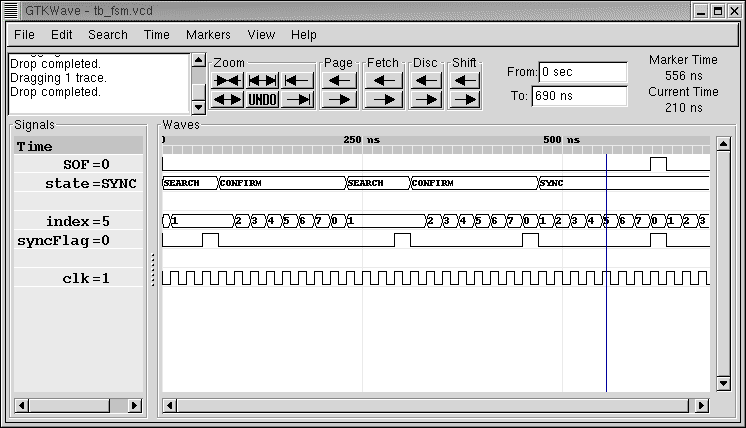
\includegraphics{tbfsm.png}
\fi

Signals are dumped in a suitable format. This format is inferred at
the \class{Signal} construction time, from the type of the initial
value. In particular, \class{bool} signals are dumped as single
bits. (This only works starting with Python~2.3, when \class{bool} has
become a separate type).  Likewise, \class{intbv} signals with a
defined bit width are dumped as bit vectors. To support the general
case, other types of signals are dumped as a string representation, as
returned by the standard \function{str()} function.

\begin{notice}[warning]
Support for literal string representations is not part of the VCD
standard. It is specific to \program{gtkwave}. To generate a
standard VCD file, you need to use signals with a defined bit width
only.
\end{notice}


\section{High level modeling \label{model-hl}}
\index{modeling!high level}

\subsection{Modeling with bus-functional procedures \label{model-bfm}}

\index{bus-functional procedure}%
A \dfn{bus-functional procedure} is a reusable encapsulation of the
low-level operations needed to implement some abstract transaction on
a physical interface. Bus-functional procedures are typically used in
flexible verification environments.

Once again, \myhdl\ uses generator functions to support
bus-functional procedures. In \myhdl\, the difference between
instances and bus-functional procedure calls comes from the way in
which a generator function is used.

As an example, we will design a bus-functional procedure of a
simplified UART transmitter. We assume 8 data bits, no parity bit, and
a single stop bit, and we add print statements to follow the
simulation behavior:

\begin{verbatim}
T_9600 = int(1e9 / 9600)

def rs232_tx(tx, data, duration=T_9600):
    
    """ Simple rs232 transmitter procedure.

    tx -- serial output data
    data -- input data byte to be transmitted
    duration -- transmit bit duration
    
    """

    print "-- Transmitting %s --" % hex(data)
    print "TX: start bit"      
    tx.next = 0
    yield delay(duration)

    for i in range(8):
        print "TX: %s" % data[i]
        tx.next = data[i]
        yield delay(duration)

    print "TX: stop bit"      
    tx.next = 1
    yield delay(duration)
\end{verbatim}

This looks exactly like the generator functions in previous sections. It
becomes a bus-functional procedure when we use it differently. Suppose
that in a test bench, we want to generate a number of data bytes to be
transmitted. This can be modeled as follows:


\begin{verbatim}
testvals = (0xc5, 0x3a, 0x4b)

def stimulus():
    tx = Signal(1)
    for val in testvals:
        txData = intbv(val)
        yield rs232_tx(tx, txData)
\end{verbatim}

We use the bus-functional procedure call as a clause in a
\code{yield} statement. This introduces a fourth form of the
\code{yield} statement: using a generator as a clause. Although this is
a more dynamic usage than in the previous cases, the meaning is
actually very similar: at that point,
the original generator should 
    \index{wait!for the completion of a generator}% 
wait for the completion of a generator. 
In this case, the original generator resumes when the
\code{rs232_tx(tx, txData)} generator returns.

When simulating this, we get:

\begin{verbatim}
-- Transmitting 0xc5 --
TX: start bit
TX: 1
TX: 0
TX: 1
TX: 0
TX: 0
TX: 0
TX: 1
TX: 1
TX: stop bit
-- Transmitting 0x3a --
TX: start bit
TX: 0
TX: 1
TX: 0
TX: 1
...
\end{verbatim}

We will continue with this example by designing the corresponding UART
receiver bus-functional procedure. This will allow us to introduce
further capabilities of \myhdl\ and its use of the \code{yield}
statement. 

Until now, the \code{yield} statements had a single clause. However,
they can have multiple clauses as well. In that case, the generator
resumes as soon as the wait condition specified by one
of the clauses is satisfied. This corresponds to the functionality of
    \index{sensitivity list}%
sensitivity lists in Verilog and VHDL.

For example, suppose we want to design an UART receive procedure with
a timeout. We can specify the timeout condition while waiting for the
start bit, as in the following generator function:

\begin{verbatim}
def rs232_rx(rx, data, duration=T_9600, timeout=MAX_TIMEOUT):
    
    """ Simple rs232 receiver procedure.

    rx -- serial input data
    data -- data received
    duration -- receive bit duration
    
    """

    # wait on start bit until timeout
    yield rx.negedge, delay(timeout)
    if rx == 1:
        raise StopSimulation, "RX time out error"

    # sample in the middle of the bit duration
    yield delay(duration // 2)
    print "RX: start bit"

    for i in range(8):
        yield delay(duration)
        print "RX: %s" % rx
        data[i] = rx

    yield delay(duration)
    print "RX: stop bit"
    print "-- Received %s --" % hex(data)
\end{verbatim}

If the timeout condition is triggered, the receive bit \code{rx}
will still be \code{1}. In that case, we raise an exception to stop
the simulation. The \code{StopSimulation} exception is predefined in
\myhdl\ for such purposes. In the other case, we proceed by
positioning the sample point in the middle of the bit duration, and
sampling the received data bits.

When a \code{yield} statement has multiple clauses, they can be of any
type that is supported as a single clause, including generators. For
example, we can verify the transmitter and receiver generator against
each other by yielding them together, as follows:

\begin{verbatim}
def test():
    tx = Signal(1)
    rx = tx
    rxData = intbv(0)
    for val in testvals:
        txData = intbv(val)
        yield rs232_rx(rx, rxData), rs232_tx(tx, txData)
\end{verbatim}

Both forked generators will run concurrently, and the original
generator will resume as soon as one of them finishes (which will be
the transmitter in this case).  The simulation output shows how
the UART procedures run in lockstep:

\begin{verbatim}
-- Transmitting 0xc5 --
TX: start bit
RX: start bit
TX: 1
RX: 1
TX: 0
RX: 0
TX: 1
RX: 1
TX: 0
RX: 0
TX: 0
RX: 0
TX: 0
RX: 0
TX: 1
RX: 1
TX: 1
RX: 1
TX: stop bit
RX: stop bit
-- Received 0xc5 --
-- Transmitting 0x3a --
TX: start bit
RX: start bit
TX: 0
RX: 0
...
\end{verbatim}

For completeness, we will verify the timeout behavior with a test
bench that disconnects the \code{rx} from the \code{tx} signal, and we
specify a small timeout for the receive procedure:

\begin{verbatim}
def testTimeout():
    tx = Signal(1)
    rx = Signal(1)
    rxData = intbv(0)
    for val in testvals:
        txData = intbv(val)
        yield rs232_rx(rx, rxData, timeout=4*T_9600-1), rs232_tx(tx, txData)
\end{verbatim}
 
The simulation now stops with a timeout exception after a few
transmit cycles:

\begin{verbatim}
-- Transmitting 0xc5 --
TX: start bit
TX: 1
TX: 0
TX: 1
StopSimulation: RX time out error
\end{verbatim}

Recall that the original generator resumes as soon as one of the
forked generators returns. In the previous cases, this is just fine,
as the transmitter and receiver generators run in lockstep. However,
it may be desirable to resume the caller only when \emph{all} of the
forked generators have finished. For example, suppose that we want to
characterize the robustness of the transmitter and receiver design to
bit duration differences. We can adapt our test bench as follows, to
run the transmitter at a faster rate:

\begin{verbatim}
T_10200 = int(1e9 / 10200)

def testNoJoin():
    tx = Signal(1)
    rx = tx
    rxData = intbv(0)
    for val in testvals:
        txData = intbv(val)
        yield rs232_rx(rx, rxData), rs232_tx(tx, txData, duration=T_10200)
\end{verbatim}

Simulating this shows how the transmission of the new byte starts
before the previous one is received, potentially creating additional
transmission errors:

\begin{verbatim}
-- Transmitting 0xc5 --
TX: start bit
RX: start bit
...
TX: 1
RX: 1
TX: 1
TX: stop bit
RX: 1
-- Transmitting 0x3a --
TX: start bit
RX: stop bit
-- Received 0xc5 --
RX: start bit
TX: 0
\end{verbatim}

It is more likely that we want to characterize the design on a byte
by byte basis, and align the two generators before transmitting each
byte. In \myhdl{}, this is done with the \function{join} function. By
joining clauses together in a \code{yield} statement, we create a new
clause that triggers only when all of its clause arguments have
triggered. For example, we can adapt the test bench as follows:

\begin{verbatim}
def testJoin():
    tx = Signal(1)
    rx = tx
    rxData = intbv(0)
    for val in testvals:
        txData = intbv(val)
        yield join(rs232_rx(rx, rxData), rs232_tx(tx, txData, duration=T_10200))
\end{verbatim}

Now, transmission of a new byte only starts when the previous one is received:

\begin{verbatim}
-- Transmitting 0xc5 --
TX: start bit
RX: start bit
...
TX: 1
RX: 1
TX: 1
TX: stop bit
RX: 1
RX: stop bit
-- Received 0xc5 --
-- Transmitting 0x3a --
TX: start bit
RX: start bit
TX: 0
RX: 0
\end{verbatim}



\subsection{Modeling memories with built-in types \label{model-mem}}
\index{modeling!memories}

Python has powerful built-in data types that can be useful to model
hardware memories. This can be merely a matter of putting an interface
around some data type operations.

For example, a \dfn{dictionary} comes in handy to model sparse memory
structures. (In other languages, this data type is called 
\dfn{associative array}, or \dfn{hash table}.) A sparse memory is one in
which only a small part of the addresses is used in a particular
application or simulation. Instead of statically allocating the full
address space, which can be large, it is better to dynamically
allocate the needed storage space. This is exactly what a dictionary
provides. The following is an example of a sparse memory model:

\begin{verbatim}
def sparseMemory(dout, din, addr, we, en, clk):
    
    """ Sparse memory model based on a dictionary.

    Ports:
    dout -- data out
    din -- data in
    addr -- address bus
    we -- write enable: write if 1, read otherwise
    en -- interface enable: enabled if 1
    clk -- clock input
    
    """

    memory = {}

    @always(clk.posedge)
    def access():
        if en:
            if we:
                memory[addr.val] = din.val
            else:
                dout.next = memory[addr.val]

    return access
\end{verbatim} 

Note how we use the \code{val} attribute of the \code{din} signal, as
we don't want to store the signal object itself, but its current
value. Similarly, we use the \code{val} attribute of the \code{addr}
signal as the dictionary key. 

In many cases, \myhdl\ code uses a signal's current value
automatically when there is no ambiguity: for example, when a signal
is used in an expression. However, in other cases such as in this
example you have to refer to the value explicitly: for example, when
the Signal is used as an index, or when it is not used in an
expression.  One option is to use the \code{val} attribute, as in this
example.  Another possibility is to use the \code{int()} or
\code{bool()} functions to typecast the Signal to an integer or a
boolean value. These functions are also useful with \class{intbv}
objects.

As a second example, we will demonstrate how to use a list to model a
synchronous fifo:

\begin{verbatim}
def fifo(dout, din, re, we, empty, full, clk, maxFilling=sys.maxint):
    
    """ Synchronous fifo model based on a list.
    
    Ports:
    dout -- data out
    din -- data in
    re -- read enable
    we -- write enable
    empty -- empty indication flag
    full -- full indication flag
    clk -- clock input

    Optional parameter:
    maxFilling -- maximum fifo filling, "infinite" by default

    """
    
    memory = []

    @always(clk.posedge)
    def access():
        if we:
            memory.insert(0, din.val)
        if re:
            dout.next = memory.pop()
        filling = len(memory)
        empty.next = (filling == 0)
        full.next = (filling == maxFilling)

    return access
\end{verbatim}

Again, the model is merely a \myhdl\ interface around some operations
on a list: \function{insert()} to insert entries, \function{pop()} to
retrieve them, and \function{len()} to get the size of a Python
object.

\subsection{Modeling errors using exceptions \label{model-err}}

In the previous section, we used Python data types for modeling. If
such a type is used inappropriately, Python's run time error system
will come into play. For example, if we access an address in the
\function{sparseMemory} model that was not initialized before, we will
get a traceback similar to the following (some lines omitted for
clarity):

\begin{verbatim}
Traceback (most recent call last):
...
  File "sparseMemory.py", line 31, in access
    dout.next = memory[addr.val]
KeyError: Signal(51)
\end{verbatim}

Similarly, if the \code{fifo} is empty, and we attempt to read from
it, we get:

\begin{verbatim}
Traceback (most recent call last):
...
  File "fifo.py", line 34, in fifo
    dout.next = memory.pop()
IndexError: pop from empty list
\end{verbatim}

Instead of these low level errors, it may be preferable to define
errors at the functional level. In Python, this is typically done by
defining a custom \code{Error} exception, by subclassing the standard
\code{Exception} class. This exception is then raised explicitly when
an error condition occurs.

For example, we can change the \function{sparseMemory} function as
follows (with the doc string is omitted for brevity):

\begin{verbatim}
class Error(Exception):
    pass

def sparseMemory2(dout, din, addr, we, en, clk):
   
    memory = {}

    @always(clk.posedge)
    def access():
        if en:
            if we:
                memory[addr.val] = din.val
            else:
                try:
                    dout.next = memory[addr.val]
                except KeyError:
                    raise Error, "Uninitialized address %s" % hex(addr)

    return access

\end{verbatim}

This works by catching the low level data type exception, and raising
the custom exception with an appropriate error message instead.  If
the \function{sparseMemory} function is defined in a module with the
same name, an access error is now reported as follows:

\begin{verbatim}
Traceback (most recent call last):
...
  File "sparseMemory.py", line 61, in access
    raise Error, "Uninitialized address %s" % hex(addr)
Error: Uninitialized address 0x33

\end{verbatim}

Likewise, the \function{fifo} function can be adapted as follows, to
report underflow and overflow errors:

\begin{verbatim}
class Error(Exception):
    pass


def fifo2(dout, din, re, we, empty, full, clk, maxFilling=sys.maxint):
 
    memory = []

    @always(clk.posedge)
    def access():
        if we:
            memory.insert(0, din.val)
        if re:
            try:
                dout.next = memory.pop()
            except IndexError:
                raise Error, "Underflow -- Read from empty fifo"
        filling = len(memory)
        empty.next = (filling == 0)
        full.next = (filling == maxFilling)
        if filling > maxFilling:
            raise Error, "Overflow -- Max filling %s exceeded" % maxFilling

    return access
\end{verbatim}

In this case, the underflow error is detected as before, by catching a
low level exception on the list data type. On the other hand, the
overflow error is detected by a regular check on the length of the
list.


\subsection{Object oriented modeling \label{model-obj}}
\index{modeling!object oriented}

The models in the previous sections used high-level built-in data
types internally. However, they had a conventional RTL-style
interface.  Communication with such a module is done through signals
that are attached to it during instantiation.

A more advanced approach is to model hardware blocks as
objects. Communication with objects is done through method calls.
A method encapsulates all details of a certain task performed
by the object. As an object has a method interface instead
of an RTL-style hardware interface, this is a much 
higher level approach.

As an example, we will design a synchronized queue object. 
Such an object can be filled by producer, and independently
read by a consumer. When the queue is empty, the consumer
should wait until an item is available. The queue can be modeled
as an object with a \method{put(item)} and a \method{get()}
method, as follows:

\begin{verbatim}
from myhdl import *

def trigger(event):
    event.next = not event

class queue:
    def __init__(self):
       self.l = []
       self.sync = Signal(0)
       self.item = None
    def put(self,item):
       # non time-consuming method
       self.l.append(item)
       trigger(self.sync)
    def get(self):
       # time-consuming method
       if not self.l:
          yield self.sync
       self.item = self.l.pop(0)
\end{verbatim}

The \class{queue} object constructor initializes an internal list to
hold items, and a \var{sync} signal to synchronize the operation
between the methods. Whenever \method{put()} puts an item in the
queue, the signal is triggered.  When the \method{get()} method sees
that the list is empty, it waits on the trigger first.
\method{get()} is a generator method because 
it may consume time. As the \code{yield} statement is used in \myhdl\
for timing control, the method cannot ``yield'' the item. Instead, it
makes it available in the \var{item} instance variable.

To test the queue operation, we will model a producer and a consumer
in the test bench.  As a waiting consumer should not block a whole
system, it should run in a concurrent ``thread''. As always in
\myhdl{}, concurrency is modeled by Python generators. Producer
and consumer will thus run independently, and we will monitor
their operation through some print statements:

\begin{verbatim}
q = queue()

def Producer(q):
    yield delay(120)
    for i in range(5):
        print "%s: PUT item %s" % (now(), i)
        q.put(i)
        yield delay(max(5, 45 - 10*i))

def Consumer(q):
    yield delay(100)
    while 1:
        print "%s: TRY to get item" % now()
        yield q.get()
        print "%s: GOT item %s" % (now(), q.item)
        yield delay(30)

def main():
    P = Producer(q)
    C = Consumer(q)
    return P, C 

sim = Simulation(main())
sim.run()
\end{verbatim}

Note that the generator method \method{get()} is called in a
\code{yield} statement in the \function{Consumer} function. The new
generator will take over from \function{Consumer}, until it is done.
Running this test bench produces the following output:

\begin{verbatim}
% python queue.py
100: TRY to get item
120: PUT item 0
120: GOT item 0
150: TRY to get item
165: PUT item 1
165: GOT item 1
195: TRY to get item
200: PUT item 2
200: GOT item 2
225: PUT item 3
230: TRY to get item
230: GOT item 3
240: PUT item 4
260: TRY to get item
260: GOT item 4
290: TRY to get item
StopSimulation: No more events
\end{verbatim}

\chapter{Unit testing \label{unittest}}

\section{Introduction \label{unittest-intro}}

Many aspects in the design flow of modern digital hardware design can
be viewed as a special kind of software development. From that
viewpoint, it is a natural question whether advances in software
design techniques can not also be applied to hardware design.

One software design approach that gets a lot of attention recently is
\index{extreme programming}%
\emph{Extreme Programming} (XP). It is a fascinating set of techniques and
guidelines that often seems to go against the conventional wisdom. On
other occasions, XP just seems to emphasize the common sense, which
doesn't always coincide with common practice. For example, XP stresses
the importance of normal workweeks, if we are to have the
fresh mind needed for good software development.

It is not my intention nor qualification to present a tutorial on
Extreme Programming. Instead, in this section I will highlight one XP
concept which I think is very relevant to hardware design: the
importance and methodology of unit testing.

\section{The importance of unit tests \label{unittest-why}}

Unit testing is one of the corner stones of Extreme Programming. Other
XP concepts, such as collective ownership of code and continuous
refinement, are only possible by having unit tests. Moreover, XP
emphasizes that writing unit tests should be automated, that they should
test everything in every class, and that they should run perfectly all
the time. 

I believe that these concepts apply directly to hardware design. In
addition, unit tests are a way to manage simulation time. For example,
a state machine that runs very slowly on infrequent events may be
impossible to verify at the system level, even on the fastest
simulator. On the other hand, it may be easy to verify it exhaustively
in a unit test, even on the slowest simulator.

It is clear that unit tests have compelling advantages. On the other
hand, if we need to test everything, we have to write
lots of unit tests. So it should be easy and pleasant
to create, manage and run them. Therefore, XP emphasizes the need for
a unit test framework that supports these tasks. In this chapter,
we will explore the use of the \code{unittest} module from
the standard Python library for creating unit tests for hardware
designs.


\section{Unit test development \label{unittest-dev}}

In this section, we will informally explore the application of unit
test techniques to hardware design. We will do so by a (small)
example: testing a binary to Gray encoder as introduced in
section~\ref{intro-indexing}. 

\subsection{Defining the requirements \label{unittest-req}}

We start by defining the requirements. For a Gray encoder, we want to
the output to comply with Gray code characteristics. Let's define a
\dfn{code} as a list of \dfn{codewords}, where a codeword is a bit
string. A code of order \code{n} has \code{2**n} codewords.

A well-known characteristic is the one that Gray codes are all about:

\newtheorem{reqGray}{Requirement}
\begin{reqGray} 
Consecutive codewords in a Gray code should differ in a single bit.
\end{reqGray}

Is this sufficient? Not quite: suppose for example that an
implementation returns the lsb of each binary input. This would comply
with the requirement, but is obviously not what we want. Also, we don't
want the bit width of Gray codewords to exceed the bit width of the
binary codewords.

\begin{reqGray} 
Each codeword in a Gray code of order n must occur exactly once in the
binary code of the same order.
\end{reqGray}

With the requirements written down we can proceed.

\subsection{Writing the test first \label{unittest-first}}

A fascinating guideline in the XP world is to write the unit test
first. That is, before implementing something, first write the test
that will verify it. This seems to go against our natural inclination,
and certainly against common practices. Many engineers like to
implement first and think about verification afterwards.

But if you think about it, it makes a lot of sense to deal with
verification first. Verification is about the requirements only --- so
your thoughts are not yet cluttered with implementation details. The
unit tests are an executable description of the requirements, so they
will be better understood and it will be very clear what needs to be
done. Consequently, the implementation should go smoother. Perhaps
most importantly, the test is available when you are done
implementing, and can be run anytime by anybody to verify changes.

Python has a standard \code{unittest} module that facilitates writing,
managing and running unit tests. With \code{unittest}, a test case is 
written by creating a class that inherits from
\code{unittest.TestCase}. Individual tests are created by methods of
that class: all method names that start with \code{test} are
considered to be tests of the test case.

We will define a test case for the Gray code properties, and then
write a test for each of the requirements. The outline of the test
case class is as follows:

\begin{verbatim}
from unittest import TestCase

class TestGrayCodeProperties(TestCase):

    def testSingleBitChange(self):
     """ Check that only one bit changes in successive codewords """
     ....


    def testUniqueCodeWords(self):
        """ Check that all codewords occur exactly once """
    ....
\end{verbatim}

Each method will be a small test bench that tests a single
requirement. To write the tests, we don't need an implementation of
the Gray encoder, but we do need the interface of the design. We can
specify this by a dummy implementation, as follows:

\begin{verbatim}
def bin2gray(B, G, width):
    ### NOT IMPLEMENTED YET! ###
    yield None
\end{verbatim}

For the first requirement, we will write a test bench that applies all
consecutive input numbers, and compares the current output with the
previous one for each input. Then we check that the difference is a
single bit. We will test all Gray codes up to a certain order
\code{MAX_WIDTH}.

\begin{verbatim}
    def testSingleBitChange(self):
        """ Check that only one bit changes in successive codewords """
        
        def test(B, G, width):
            B.next = intbv(0)
            yield delay(10)
            for i in range(1, 2**width):
                G_Z.next = G
                B.next = intbv(i)
                yield delay(10)
                diffcode = bin(G ^ G_Z)
                self.assertEqual(diffcode.count('1'), 1)
        
        for width in range(1, MAX_WIDTH):
            B = Signal(intbv(-1))
            G = Signal(intbv(0))
            G_Z = Signal(intbv(0))
            dut = bin2gray(B, G, width)
            check = test(B, G, width)
            sim = Simulation(dut, check)
            sim.run(quiet=1)
\end{verbatim}

Note how the actual check is performed by a \code{self.assertEqual}
method, defined by the \code{unittest.TestCase} class.

Similarly, we write a test bench for the second requirement. Again, we
simulate all numbers, and put the result in a list. The requirement
implies that if we sort the result list, we should get a range of
numbers:

\begin{verbatim}
    def testUniqueCodeWords(self):
        """ Check that all codewords occur exactly once """

        def test(B, G, width):
            actual = []
            for i in range(2**width):
                B.next = intbv(i)
                yield delay(10)
                actual.append(int(G))
            actual.sort()
            expected = range(2**width)
            self.assertEqual(actual, expected)
       
        for width in range(1, MAX_WIDTH):
            B = Signal(intbv(-1))
            G = Signal(intbv(0))
            dut = bin2gray(B, G, width)
            check = test(B, G, width)
            sim = Simulation(dut, check)
            sim.run(quiet=1)
\end{verbatim}


\subsection{Test-driven implementation \label{unittest-impl}}

With the test written, we begin with the implementation. For
illustration purposes, we will intentionally write some incorrect
implementations to see how the test behaves.

The easiest way to run tests defined with the \code{unittest}
framework, is to put a call to its \code{main} method at the end of
the test module:

\begin{verbatim}
unittest.main()
\end{verbatim}

Let's run the test using the dummy Gray encoder shown earlier:

\begin{verbatim}
% python test_gray.py -v
Check that only one bit changes in successive codewords ... FAIL
Check that all codewords occur exactly once ... FAIL
<trace backs not shown>
\end{verbatim}

As expected, this fails completely. Let us try an incorrect
implementation, that puts the lsb of in the input on the output:

\begin{verbatim}
def bin2gray(B, G, width):
    ### INCORRECT - DEMO PURPOSE ONLY! ###

    @always_comb
    def logic():
        G.next = B[0]

    return logic
\end{verbatim}


Running the test produces:

\begin{verbatim}
% python test_gray.py -v
Check that only one bit changes in successive codewords ... ok
Check that all codewords occur exactly once ... FAIL

======================================================================
FAIL: Check that all codewords occur exactly once
----------------------------------------------------------------------
Traceback (most recent call last):
  File "test_gray.py", line 109, in testUniqueCodeWords
    sim.run(quiet=1)
...
  File "test_gray.py", line 104, in test
    self.assertEqual(actual, expected)
  File "/usr/local/lib/python2.2/unittest.py", line 286, in failUnlessEqual
    raise self.failureException, \
AssertionError: [0, 0, 1, 1] != [0, 1, 2, 3]

----------------------------------------------------------------------
Ran 2 tests in 0.785s
\end{verbatim}

Now the test passes the first requirement, as expected, but fails the
second one. After the test feedback, a full traceback is shown that
can help to debug the test output.

Finally, if we use the correct implementation as in
section~\ref{intro-indexing}, the output is:

\begin{verbatim}
% python test_gray.py -v
Check that only one bit changes in successive codewords ... ok
Check that all codewords occur exactly once ... ok

----------------------------------------------------------------------
Ran 2 tests in 6.364s

OK
\end{verbatim}



\subsection{Changing requirements \label{unittest-change}}

In the previous section, we concentrated on the general requirements
of a Gray code. It is possible to specify these without specifying the
actual code. It is easy to see that there are several codes
that satisfy these requirements. In good XP style, we only tested
the requirements and nothing more.

It may be that more control is needed. For example, the requirement
may be for a particular code, instead of compliance with general
properties. As an illustration, we will show how to test for
\emph{the} original Gray code, which is one specific instance that
satisfies the requirements of the previous section. In this particular
case, this test will actually be easier than the previous one.

We denote the original Gray code of order \code{n} as \code{Ln}. Some
examples: 

\begin{verbatim}
L1 = ['0', '1']
L2 = ['00', '01', '11', '10']
L3 = ['000', '001', '011', '010', '110', '111', '101', 100']
\end{verbatim}

It is possible to specify these codes by a recursive algorithm, as
follows:

\begin{enumerate}
\item L1 = ['0', '1']
\item Ln+1 can be obtained from Ln as follows. Create a new code Ln0 by
prefixing all codewords of Ln with '0'. Create another new code Ln1 by
prefixing all codewords of Ln with '1', and reversing their
order. Ln+1 is the concatenation of Ln0 and Ln1.
\end{enumerate}

Python is well-known for its elegant algorithmic
descriptions, and this is a good example. We can write the algorithm
in Python as follows:

\begin{verbatim}
def nextLn(Ln):
    """ Return Gray code Ln+1, given Ln. """
    Ln0 = ['0' + codeword for codeword in Ln]
    Ln1 = ['1' + codeword for codeword in Ln]
    Ln1.reverse()
    return Ln0 + Ln1
\end{verbatim}

The code \samp{['0' + codeword for ...]} is called a \dfn{list
comprehension}. It is a concise way to describe lists built by short
computations in a for loop.

The requirement is now that the output code matches the
expected code Ln. We use the \code{nextLn} function to compute the
expected result. The new test case code is as follows:

\begin{verbatim}
class TestOriginalGrayCode(TestCase):

    def testOriginalGrayCode(self):
        """ Check that the code is an original Gray code """

        Rn = []
        
        def stimulus(B, G, n):
            for i in range(2**n):
                B.next = intbv(i)
                yield delay(10)
                Rn.append(bin(G, width=n))
        
        Ln = ['0', '1'] # n == 1
        for n in range(2, MAX_WIDTH):
            Ln = nextLn(Ln)
            del Rn[:]
            B = Signal(intbv(-1))
            G = Signal(intbv(0))
            dut = bin2gray(B, G, n)
            stim = stimulus(B, G, n)
            sim = Simulation(dut, stim)
            sim.run(quiet=1)
            self.assertEqual(Ln, Rn)
\end{verbatim}

As it happens, our implementation is apparently an original Gray code:

\begin{verbatim}
% python test_gray.py -v TestOriginalGrayCode
Check that the code is an original Gray code ... ok

----------------------------------------------------------------------
Ran 1 tests in 3.091s

OK
\end{verbatim}


 


\chapter{Co-simulation with Verilog and VHDL \label{cosim}}

\section{Introduction \label{cosim-intro}}

One of the most exciting possibilities of \myhdl\
is to use it as a hardware verification language (HVL).
A HVL is a language used to write test benches and
verification environments, and to control simulations.

Nowadays, it is generally acknowledged that HVLs should be equipped
with modern software techniques, such as object orientation. The
reason is that verification it the most complex and time-consuming
task of the design process. Consequently, every useful technique is
welcome. Moreover, test benches are not required to be
implementable. Therefore, unlike with synthesizable code, there
are no constraints on creativity.

Technically, verification of a design implemented in
another language requires co-simulation. \myhdl\ is 
enabled for co-simulation with any HDL simulator that
has a procedural language interface (PLI). The \myhdl\
side is designed to be independent of a particular
simulator, On the other hand, for each HDL simulator a specific
PLI module will have to be written in C. Currently,
the \myhdl\ release contains a PLI module for
two Verilog simulators: Icarus and Cver.

\section{The HDL side \label{cosim-hdl}}

To introduce co-simulation, we will continue to use the Gray encoder
example from the previous chapters. Suppose that we want to
synthesize it and write it in Verilog for that purpose. Clearly we would
like to reuse our unit test verification environment. 

To start, let's recall how the Gray encoder in \myhdl{} looks like:

\begin{verbatim}
def bin2gray(B, G, width):
    """ Gray encoder.

    B -- input intbv signal, binary encoded
    G -- output intbv signal, gray encoded
    width -- bit width
    """

    @always_comb
    def logic():
        for i in range(width):
            G.next[i] = B[i+1] ^ B[i]

    return logic
\end{verbatim}

To show the co-simulation flow, we don't need the Verilog
implementation yet, but only the interface.  Our Gray encoder in
Verilog would have the following interface:

\begin{verbatim}
module bin2gray(B, G);

   parameter width = 8;
   input [width-1:0]  B;     
   output [width-1:0] G;
   ....
\end{verbatim}

To write a test bench, one creates a new module that instantiates the
design under test (DUT).  The test bench declares nets and
regs (or signals in VHDL) that are attached to the DUT, and to
stimulus generators and response checkers. In an all-HDL flow, the
generators and checkers are written in the HDL itself, but we will
want to write them in \myhdl{}. To make the connection, we need to
declare which regs \& nets are driven and read by the \myhdl\
simulator. For our example, this is done as follows:

\begin{verbatim}
module dut_bin2gray;

   reg [`width-1:0] B;
   wire [`width-1:0] G;

   initial begin
      $from_myhdl(B);
      $to_myhdl(G);
   end

   bin2gray dut (.B(B), .G(G));
   defparam dut.width = `width;

endmodule
\end{verbatim}

The \code{\$from_myhdl} task call declares which regs are driven by
\myhdl{}, and the \code{\$to_myhdl} task call which regs \& nets are read
by it. These tasks take an arbitrary number of arguments.  They are
defined in a PLI module written in C and made available in a
simulator-dependent manner.  In Icarus Verilog, the tasks are defined
in a \code{myhdl.vpi} module that is compiled from C source code.

\section{The \myhdl\ side \label{cosim-myhdl}}

\myhdl\ supports co-simulation by a \code{Cosimulation} object. 
A \code{Cosimulation} object must know how to run a HDL simulation.
Therefore, the first argument to its constructor is a command string
to execute a simulation.

The way to generate and run an simulation executable is simulator
dependent.  For example, in Icarus Verilog, a simulation executable
for our example can be obtained obtained by running the
\code{iverilog} compiler as follows:

\begin{verbatim}
% iverilog -o bin2gray -Dwidth=4 bin2gray.v dut_bin2gray.v
\end{verbatim}

This generates a \code{bin2gray} executable for a parameter \code{width}
of 4, by compiling the contributing verilog files.

The simulation itself is run by the \code{vvp} command:

\begin{verbatim}
% vvp -m ./myhdl.vpi bin2gray
\end{verbatim}

This runs the \code{bin2gray} simulation, and specifies to use the
\code{myhdl.vpi} PLI module present in the current directory. (This is 
just a command line usage example; actually simulating with the
\code{myhdl.vpi} module is only meaningful from a
\code{Cosimulation} object.)

We can use a \code{Cosimulation} object to provide a HDL
version of a design to the \myhdl\ simulator. Instead of a generator
function, we write a function that returns a \code{Cosimulation}
object. For our example and the Icarus Verilog simulator, this is done
as follows:

\begin{verbatim}
import os

from myhdl import Cosimulation

cmd = "iverilog -o bin2gray -Dwidth=%s bin2gray.v dut_bin2gray.v"
      
def bin2gray(B, G, width):
    os.system(cmd % width)
    return Cosimulation("vvp -m ./myhdl.vpi bin2gray", B=B, G=G)
\end{verbatim}

After the executable command argument, the \code{Cosimulation}
constructor takes an arbitrary number of keyword arguments. Those
arguments make the link between \myhdl\ Signals and HDL nets, regs, or
signals, by named association. The keyword is the name of an argument
in a \code{\$to_myhdl} or \code{\$from_myhdl} call; the argument is
a \myhdl\ Signal.

With all this in place, we can now use the existing unit test
to verify the Verilog implementation. Note that we kept the
same name and parameters for the the \code{bin2gray} function:
all we need to do is to provide this alternative definition
to the existing unit test.

Let's try it on the Verilog design:

\begin{verbatim}
module bin2gray(B, G);

   parameter width = 8;
   input [width-1:0]  B;
   output [width-1:0] G;
   reg [width-1:0] G;
   integer i;
   wire [width:0] extB;

   assign extB = {1'b0, B}; // zero-extend input

   always @(extB) begin
      for (i=0; i < width; i=i+1)
        G[i] <= extB[i+1] ^ extB[i];
   end

endmodule
\end{verbatim}

When we run our unit test, we get:

\begin{verbatim}
% python test_bin2gray.py 
Check that only one bit changes in successive codewords ... ok
Check that all codewords occur exactly once ... ok
Check that the code is an original Gray code ... ok

----------------------------------------------------------------------
Ran 3 tests in 2.729s

OK
\end{verbatim}


\section{Restrictions \label{cosim-restr}}

In the ideal case, it should be possible to simulate
any HDL description seamlessly with \myhdl{}. Moreover
the communicating signals at each side should act
transparently as a single one, enabling fully race free
operation.

For various reasons, it may not be possible or desirable
to achieve full generality. As anyone that has developed
applications with the Verilog PLI can testify, the
restrictions in a particular simulator, and the 
differences over various simulators, can be quite 
frustrating. Moreover, full generality may require
a disproportionate amount of development work compared
to a slightly less general solution that may
be sufficient for the target application.

Consequently, I have tried to achieve a solution
which is simple enough so that one can reasonably 
expect that any PLI-enabled simulator can support it,
and that is relatively easy to verify and maintain.
At the same time, the solution is sufficiently general 
to cover the target application space.

The result is a compromise that places certain restrictions
on the HDL code. In this section, these restrictions 
are presented.

\subsection{Only passive HDL can be co-simulated \label{cosim-pass}}

The most important restriction of the \myhdl\ co-simulation solution is
that only ``passive'' HDL can be co-simulated.  This means that the HDL
code should not contain any statements with time delays. In other
words, the \myhdl\ simulator should be the master of time; in
particular, any clock signal should be generated at the \myhdl\ side.

At first this may seem like an important restriction, but if one
considers the target application for co-simulation, it probably
isn't. 

\myhdl\ supports co-simulation so that test benches for HDL
designs can be written in Python.  Let's consider the nature of the
target HDL designs. For high-level, behavioral models that are not
intended for implementation, it should come as no surprise that I
would recommend to write them in \myhdl\ directly; that is one of the
goals of the \myhdl\ effort. Likewise, gate level designs with
annotated timing are not the target application: static timing
analysis is a much better verification method for such designs.

Rather, the targeted HDL designs are naturally models that are
intended for implementation, most likely through synthesis. As time
delays are meaningless in synthesizable code, the restriction is
compatible with the target application.

\subsection{Race sensitivity issues \label{cosim-race}}

In a typical RTL code, some events cause other events to occur in the
same time step. For example, when a clock signal triggers some signals
may change in the same time step. For race-free operation, an HDL
must differentiate between such events within a time step. This is done
by the concept of ``delta'' cycles. In a fully general, race free
co-simulation, the co-simulators would communicate at the level of delta
cycles. However, in \myhdl\ co-simulation, this is not entirely the
case.

Delta cycles from the \myhdl\ simulator toward the HDL co-simulator are
preserved. However, in the opposite direction, they are not. The
signals changes are only returned to the \myhdl\ simulator after all delta
cycles have been performed in the HDL co-simulator.

What does this mean? Let's start with the good news. As explained in
the previous section, the concept behind \myhdl\ co-simulation implies
that clocks are generated at the \myhdl\ side.  \emph{When using a
\myhdl\ clock and its corresponding HDL signal directly as a clock,
co-simulation is race free.} In other words, the case
that most closely reflects the \myhdl\ co-simulation approach, is race free.

The situation is different when you want to use a signal driven by the
HDL (and the corresponding MyHDL signal) as a clock. 
Communication triggered by such a clock is not race free. The solution
is to treat such an interface as a chip interface instead of an RTL
interface.  For example, when data is triggered at positive clock
edges, it can safely be sampled at negative clock edges.
Alternatively, the \myhdl\ data signals can be declared with a delay
value, so that they are guaranteed to change after the clock
edge.


\section{Implementation notes \label{cosim-impl}}

\begin{quote}
\em
This section requires some knowledge of PLI terminology.
\end{quote}

Enabling a simulator for co-simulation requires a PLI module written
in C. In Verilog, the PLI is part of the ``standard''.  However,
different simulators implement different versions and portions of the
standard. Worse yet, the behavior of certain PLI callbacks is not
defined on some essential points.  As a result, one should plan to
write or at least customize a specific PLI module for any simulator.
The release contains a PLI module for the open source Icarus
and Cver simulators. 

This section documents the current approach and status of the PLI
module implementation and some reflections on future
implementations.

\subsection{Icarus Verilog \label{cosim-icarus}}

\subsubsection{Delta cycle implementation \label{cosim-icarus-delta}}

To make co-simulation work, a specific type of PLI callback is
needed. The callback should be run when all pending events have been
processed, while allowing the creation of new events in the current
time step (e.g. by the \myhdl\ simulator).  In some Verilog
simulators, the \code{cbReadWriteSync} callback does exactly
that. However, in others, including Icarus, it does not. The
callback's behavior is not fully standardized; some simulators run the
callback before non-blocking assignment events have been processed.

Consequently, I had to look for a workaround. One half of the solution
is to use the \code{cbReadOnlySync} callback.  This callback runs
after all pending events have been processed.  However, it does not
permit to create new events in the current time step.  The second half
of the solution is to map \myhdl\ delta cycles onto real Verilog time
steps.  Note that fortunately I had some freedom here because of the
restriction that only passive HDL code can be co-simulated.

I chose to make the time granularity in the Verilog simulator a 1000
times finer than in the \myhdl{} simulator. For each \myhdl\ time
step, 1000 Verilog time steps are available for \myhdl\ delta
cycles. In practice, only a few delta cycles per time step should be
needed. Exceeding this limit almost certainly indicates a design error;
the limit is checked at run-time. The factor 1000 also makes it
easy to distinguish ``real'' time from delta cycle time when printing
out the Verilog time.

\subsubsection{Passive Verilog check \label{cosim-icarus-pass}}

As explained before, co-simulated Verilog should not contain delay
statements. Ideally, there should be a run-time check to flag
non-compliant code. However, there is currently no such check in the
Icarus module.

The check can be written using the \code{cbNextSimTime} VPI callback
in Verilog. However, Icarus 0.7 doesn't support this callback. In the
meantime, support for it has been added to the Icarus development
branch.  When Icarus 0.8 is released, a check will be added.

In the mean time, just don't do this. It may appear to ``work'' but it
really won't as events will be missed over the co-simulation
interface.


\subsection{Cver \label{cosim-cver}}

MyHDL co-simulation is supported with the open source Verilog
simulator Cver. The PLI module is based on the one for Icarus
and basically has the same functionality. Only some cosmetic
modifications were required.

\subsection{Other Verilog simulators \label{cosim-impl-verilog}}

The Icarus module is written with VPI calls, which are provided by the
most recent generation of the Verilog PLI. Some simulators may only
support TF/ACC calls, requiring a complete redesign of the interface
module.

If the simulator supports VPI, the Icarus module should be reusable to
a large extent. However, it may be possible to improve on it.  The
workaround to support delta cycles described in
Section~\ref{cosim-icarus-delta} may not be necessary. In some
simulators, the \code{cbReadWriteSync} callback occurs after all
events (including non-blocking assignments) have been processed. In
that case, the functionality can be supported without a finer time
granularity in the Verilog simulator.

There are also Verilog standardization efforts underway to resolve the
ambiguity of the \code{cbReadWriteSync} callback. The solution will be
to introduce new, well defined callbacks. From reading some proposals,
I conclude that the \code{cbEndOfSimTime} callback would provide the
required functionality.

The MyHDL project currently has no access to commercial Verilog
simulators, so progress in co-simulation support depends on external
interest and participation. Users have reported that they are using
MyHDL co-simulation with the simulators from Aldec and Modelsim.


\subsection{Interrupted system calls \label{cosim-impl-syscalls}}

The PLI module uses \code{read} and \code{write} system calls to
communicate between the co-simulators. The implementation assumes that
these calls are restarted automatically by the operating system when
interrupted. This is apparently what happens on the Linux box on which
MyHDL is developed.

It is known how non-restarted interrupted system calls should be
handled, but currently such code cannot be tested on the MyHDL
development platform. Also, it is not clear whether this is still a
relevant issue with modern operating systems. Therefore, this issue
has not been addressed at this moment. However, assertions have been
included that should trigger when this situation occurs.

Whenever an assertion fires in the PLI module, please report it.  The
same holds for Python exceptions that cannot be easily explained.

\subsection{VHDL \label{cosim-impl-vhdl}}

It would be nice to have an interface to VHDL simulators such as the
Modelsim VHDL simulator. This will require a PLI module using the
PLI of the VHDL simulator. 

The MyHDL project currently has no access to commercial VHDL
simulators, so progress in co-simulation support will depend on
external interest and participation.


\chapter{Conversion to Verilog\label{conv}}
\section{Introduction\label{conv-intro}}

\myhdl\ supports the automatic conversion of implementation-oriented
\myhdl\ code to Verilog code. This feature provides a
direct path from Python to an FPGA or ASIC implementation.

\section{Solution description\label{conv-solution}}

The solution works as follows. The hardware description should
satisfy certain constraints that are typical for
implementation-oriented hardware modeling.  Subsequently, such a
design is converted to an equivalent model in the Verilog language,
using the function \function{toVerilog} from the \myhdl\
library. Finally, a third-party \emph{synthesis tool} is used to
convert the Verilog design to a gate implementation for an ASIC or
FPGA. There are a number of Verilog synthesis tools available, varying
in price, capabilities, and target implementation technology.

The conversion does not start from source files, but from an
instantiated design that has been \emph{elaborated} by the Python
interpreter. The converter uses the Python profiler to track the
interpreter's operation and to infer the design structure and name
spaces. It then selectively compiles pieces of source code for
additional analysis and for conversion. This is done using the Python
compiler package.

\section{Features\label{conv-features}}

\subsection{The design is converted after elaboration\label{conv-features-elab}}
\emph{Elaboration} refers to the initial processing of a hardware
description to achieve a representation of a design instance that is
ready for simulation or synthesis. In particular, structural
parameters and constructs are processed in this step. In \myhdl{}, the
Python interpreter itself is used for elaboration.  A
\class{Simulation} object is constructed with elaborated design
instances as arguments.  Likewise, the Verilog conversion works on an
elaborated design instance. The Python interpreter is thus used as
much as possible.

\subsection{The structural description can be arbitrarily complex and hierarchical\label{conv-features-struc}}
As the conversion works on an elaborated design instance, any modeling
constraints only apply to the leaf elements of the design structure,
that is, the co-operating generators. In other words, there are no
restrictions on the description of the design structure: Python's full
power can be used for that purpose. Also, the design hierarchy can be
arbitrarily deep.

\subsection{Generators are mapped to Verilog always or initial blocks\label{conv-features-gen}}
The converter analyzes the code of each generator and maps it
to a Verilog \code{always} blocks if possible, and to 
an \code{initial} block otherwise.
The converted Verilog design will be a flat
"net list of blocks".

\subsection{The Verilog module interface is inferred from signal usage\label{conv-features-intf}}
In \myhdl{}, the input or output direction of interface signals
is not explicitly declared. The converter investigates signal usage
in the design hierarchy to infer whether a signal is used as
input, output, or as an internal signal. Internal signals are
given a hierarchical name in the Verilog output.

\subsection{Function calls are mapped to a unique Verilog function or task call\label{conv-features-func}}
The converter analyzes function calls and function code to see if they
should be mapped to Verilog functions or to tasks. Python functions
are much more powerful than Verilog subprograms; for example, they are
inherently generic, and they can be called with named association.  To
support this power in Verilog, a unique Verilog function or task is
generated per Python function call.

\subsection{If-then-else structures may be mapped to Verilog case statements\label{conv-features-if}}
Python does not provide a case statement. However, 
the converter recognizes if-then-else structures in which a variable is
sequentially compared to items of an enumeration type, and maps
such a structure to a Verilog case statement with the appropriate
synthesis attributes.

\subsection{Choice of encoding schemes for enumeration types\label{conv-features-enum}}
The \function{enum} function in \myhdl\ returns an enumeration type. This
function takes an additional parameter \var{encoding} that specifies the
desired encoding in the implementation: binary, one hot, or one cold.
The Verilog converter generates the appropriate code.

\subsection{Support for RAM inference \label{conf-features-ram}}
Certain synthesis tools can map Verilog memories to RAM
structures. To support this interesting feature, the Verilog converter
maps lists of signals to Verilog memories.

\subsection{Support for ROM memory \label{conf-features-rom}}
Some synthesis tools can infer a ROM
from a case statement. The Verilog converter does the expansion into
a case statement automatically, based on a higher level
description. The ROM access is described in a single line, by
indexing into a tuple of integers.

\subsection{Support for signed arithmetic \label{conf-features-signed}}
In MyHDL, working with negative numbers is trivial: one just uses
\code{intbv} objects with negative values.
By contrast, negative numbers are tricky in Verilog. The language
makes a difference between an unsigned and a signed representation,
and the user has to declare signed variables explicitly.  When the two
representations are mixed in an expression, all operands are
interpreted as unsigned, which typically leads to unexpected results.

The Verilog converter handles negative \code{intbv} objects by using
a signed Verilog representation. Also, it automatically performs sign
extension and casting to a signed representation when unsigned numbers
are used in a mixed expression. In this way, it automates a task which
is notoriously hard to get right in Verilog directly.

\subsection{Support for user-defined Verilog code \label{conf-features-udfv}}
If desired, the user can bypass the regular Verilog conversion
and describe user-defined code to be inserted instead.

\section{The convertible subset\label{conv-subset}}

\subsection{Introduction\label{conv-subset-intro}}

Unsurprisingly, not all \myhdl\ code can be converted to Verilog. In
fact, there are very important restrictions.  As the goal of the
conversion functionality is implementation, this should not be a big
issue: anyone familiar with synthesis is used to similar restrictions
in the \emph{synthesizable subset} of Verilog and VHDL. The converter
attempts to issue clear error messages when it encounters a construct
that cannot be converted. 

In practice, the synthesizable subset usually refers to RTL synthesis,
which is by far the most popular type of synthesis today. There are
industry standards that define the RTL synthesis subset.  However,
those were not used as a model for the restrictions of the MyHDL
converter, but as a minimal starting point.  On that basis, whenever
it was judged easy or useful to support an additional feature, this
was done. For example, it is actually easier to convert
\keyword{while} loops than \keyword{for} loops even though they are
not RTL-synthesizable.  As another example, \keyword{print} is
supported because it's so useful for debugging, even though it's not
synthesizable.  In summary, the convertible subset is a superset of
the standard RTL synthesis subset, and supports synthesis tools with
more advanced capabilities, such as behavioral synthesis.

Recall that any restrictions only apply to the design post
elaboration.  In practice, this means that they apply only to the code
of the generators, that are the leaf functional blocks in a MyHDL
design.

\subsection{Coding style\label{conv-subset-style}}

A natural restriction on convertible code is that it should be
written in MyHDL style: cooperating generators, communicating through
signals, and with sensitivity lists specifying wait points and resume
conditions.  Supported resume conditions are a signal edge, a signal
change, or a tuple of such conditions.

\subsection{Supported types\label{conv-subset-types}}

The most important restriction regards object types. Verilog is an
almost typeless language, while Python is strongly (albeit
dynamically) typed. The converter has to infer the types of names
used in the code, and map those names to Verilog variables.

Only a limited amount of types can be converted.
Python \class{int} and \class{long} objects are mapped to Verilog
integers. All other supported types are mapped to Verilog regs (or
wires), and therefore need to have a defined bit width. The supported
types are the Python \class{bool} type, the MyHDL \class{intbv} type,
and MyHDL enumeration types returned by function \function{enum}. The
latter objects can also be used as the base object of a
\class{Signal}. 

\class{intbv} objects must be constructed so that a bit
width can be inferred. This can be done by specifying minimum
and maximum values, e.g. as follows:

\begin{verbatim}
index = intbv(0, min=MIN, max=MAX)
\end{verbatim}

The Verilog converter supports \class{intbv} objects that
can take negative values.

Alternatively, a slice can be taken from an \class{intbv} object
as follows:

\begin{verbatim}
index = intbv(0)[N:]
\end{verbatim}

Such as slice returns a new \class{intbv} object, with minimum
value \code{0} , and maximum value \code{2**N}.


\subsection{Supported statements\label{conv-subset-statements}}

The following is a list of the statements that are supported by the
Verilog converter, possibly qualified with restrictions
or usage notes. 

\begin{description}

\item[\keyword{break}]

\item[\keyword{continue}]

\item[\keyword{def}]

\item[\keyword{for}]
The only supported iteration scheme is iterating through sequences of
integers returned by built-in function \function{range} or \myhdl\
function \function{downrange}.  The optional \keyword{else} clause is
not supported.

\item[\keyword{if}]
\keyword{if}, \keyword{elif}, and \keyword{else} clauses
are fully supported.

\item[\keyword{pass}]

\item[\keyword{print}]
When printing an interpolated string, the format specifiers are copied
verbatim to the Verilog output.  Printing to a file (with syntax
\code{'>>'}) is not supported.

\item[\keyword{raise}]
This statement is mapped to Verilog statements
that end the simulation with an error message.

\item[\keyword{return}]

\item[\keyword{yield}] 
The yielded expression can be a signal, a signal edge
as specified by \myhdl\ functions \function{posedge}
or \function{negedge}, or a tuple of signals and
edge specifications.

\item[\keyword{while}]
The optional \keyword{else}
clause is not supported.

\end{description}

\subsection{Supported built-in functions\label{conv-subset-builtin}}

The following is a list of the built-in functions that are supported by the
Verilog converter.

\begin{description}
\item[\function{bool()}]
This function can be used to typecast an object explictly to
its boolean interpretation.

\item[\function{len()}]
For \class{Signal} and \class{intbv} objects, function \function{len()}
returns the bit width.

\item[\function{int()}]
This function can be used to typecast an object explictly to
its integer interpretation.

\end{description}

\subsection{Excluding code from conversion \label{conv-subset-exclude}}
For some tasks, such as debugging, it may be useful to insert arbitratry
Python code that should not be converted.

The Verilog convertor supports this by ignoring all code that is
embedded in a \code{if __debug__} test. The value of the
\code{__debug__} variable is not taken into account.

\section{Methodology notes\label{conv-meth}}

\subsection{Simulation\label{conv-meth-sim}}

In the Python philosophy, the run-time rules. The Python compiler
doesn't attempt to detect a lot of errors beyond syntax errors, which
given Python's ultra-dynamic nature would be an almost impossible task
anyway. To verify a Python program, one should run it, preferably
using unit testing to verify each feature.

The same philosophy should be used when converting a MyHDL description
to Verilog: make sure the simulation runs fine first. Although the
converter checks many things and attempts to issue clear error
messages, there is no guarantee that it does a meaningful job unless
the simulation runs fine.

\subsection{Conversion output verification\label{conv-meth-conv}}
It is always prudent to verify the converted Verilog output.
To make this task easier, the converter also generates a
test bench that makes it possible to simulate the Verilog
design using the Verilog co-simulation interface. This 
permits to verify the Verilog code with the same test
bench used for the \myhdl\ code. This is also how
the Verilog converter development is being verified.

\subsection{Assignment issues\label{conv-meth-assign}}

\subsubsection{Name assignment in Python\label{conv-meth-assign-python}}

Name assignment in Python is a different concept than in
many other languages. This point is very important for
effective modeling in Python, and even more so
for synthesizable \myhdl\ code. Therefore, the issues are
discussed here explicitly.

Consider the following name assignments:

\begin{verbatim}
a = 4
a = ``a string''
a = False
\end{verbatim}

In many languages, the meaning would be that an
existing variable \var{a} gets a number of different values.
In Python, such a concept of a variable doesn't exist. Instead,
assignment merely creates a new binding of a name to a
certain object, that replaces any previous binding.
So in the example, the name \var{a} is bound a 
number of different objects in sequence.

The Verilog converter has to investigate name
assignment and usage in \myhdl\ code, and to map
names to Verilog variables. To achieve that,
it tries to infer the type and possibly the
bit width of each expression that is assigned
to a name.

Multiple assignments to the same name can be supported if it can be
determined that a consistent type and bit width is being used in the
assignments. This can be done for boolean expressions, numeric
expressions, and enumeration type literals. In Verilog, the
corresponding name is mapped to a single bit \code{reg}, an
\code{integer}, or a \code{reg} with the appropriate width, respectively.

In other cases, a single assignment should be used when an object is
created. Subsequent value changes are then achieved by modification of
an existing object.  This technique should be used for \class{Signal}
and \class{intbv} objects.

\subsubsection{Signal assignment\label{conv-meth-assign-signal}}

Signal assignment in \myhdl\ is implemented using attribute assignment
to attribute \code{next}.  Value changes are thus modeled by
modification of the existing object. The converter investigates the
\class{Signal} object to infer the type and bit width of the
corresponding Verilog variable.

\subsubsection{\class{intbv} objects\label{conv-meth-assign-intbv}}

Type \class{intbv} is likely to be the workhorse for synthesizable
modeling in \myhdl{}. An \class{intbv} instance behaves like a
(mutable) integer whose individual bits can be accessed and
modified. Also, it is possible to constrain its set of values. In
addition to error checking, this makes it possible to infer a bit
width, which is required for implementation.

In Verilog, an \class{intbv} instance will be mapped to a \code{reg}
with an appropriate width. As noted before, it is not possible
to modify its value using name assignment. In the following, we
will show how it can be done instead. Consider:

\begin{verbatim}
a = intbv(0)[8:]
\end{verbatim}

This is an \class{intbv} object with initial value \code{0} and
bit width 8. The change its value to \code{5}, we can use
slice assignment:

\begin{verbatim}
a[8:] = 5
\end{verbatim}

The same can be achieved by leaving the bit width unspecified, 
which has the meaning to change ``all'' bits:

\begin{verbatim}
a[:] = 5
\end{verbatim}

Often the new value will depend on the old one. For example,
to increment an \class{intbv} with the technique above:

\begin{verbatim}
a[:] = a + 1
\end{verbatim}

Python also provides \emph{augmented} assignment operators,
which can be used to implement in-place operations. These are supported
on \class{intbv} objects and by the converter, so that the increment
can also be done as follows:

\begin{verbatim}
a += 1
\end{verbatim}

\section{Converter usage\label{conv-usage}}

We will demonstrate the conversion process by showing some examples.

\subsection{A small sequential design\label{conv-usage-seq}}

Consider the following MyHDL code for an incrementer module:

\begin{verbatim}
ACTIVE_LOW, INACTIVE_HIGH = 0, 1

def inc(count, enable, clock, reset, n):
    
    """ Incrementer with enable.
    
    count -- output
    enable -- control input, increment when 1
    clock -- clock input
    reset -- asynchronous reset input
    n -- counter max value
    
    """
    
    @always(clock.posedge, reset.negedge)
    def incProcess():
        if reset == ACTIVE_LOW:
            count.next = 0
        else:
            if enable:
                count.next = (count + 1) % n
                
    return incProcess
\end{verbatim}

In Verilog terminology, function \function{inc} corresponds to a
module, while the decorated function \function{incProcess}
roughly corresponds to an always block.

Normally, to simulate the design, we would "elaborate" an instance
as follows:

\begin{verbatim}
m = 8
n = 2 ** m
 
count = Signal(intbv(0)[m:])
enable = Signal(bool(0))
clock, reset = [Signal(bool()) for i in range(2)]

inc_inst = inc(count, enable, clock, reset, n=n)
\end{verbatim}

\code{inc_inst} is an elaborated design instance that can be simulated. To
convert it to Verilog, we change the last line as follows:

\begin{verbatim}
inc_inst = toVerilog(inc, count, enable, clock, reset, n=n)
\end{verbatim}

Again, this creates an instance that can be simulated, but as a side
effect, it also generates an equivalent Verilog module in file \file{inc.v}.
The Verilog code looks as follows:

\begin{verbatim}
module inc_inst (
    count,
    enable,
    clock,
    reset
);

output [7:0] count;
reg [7:0] count;
input enable;
input clock;
input reset;


always @(posedge clock or negedge reset) begin: _MYHDL1_BLOCK
    if ((reset == 0)) begin
        count <= 0;
    end
    else begin
        if (enable) begin
            count <= ((count + 1) % 256);
        end
    end
end

endmodule
\end{verbatim}

You can see the module interface and the always block, as expected
from the MyHDL design. 

\subsection{A small combinatorial design\label{conv-usage-comb}}

The second example is a small combinatorial design, more
specifically the binary to Gray code converter from previous chapters:

\begin{verbatim}
def bin2gray(B, G, width):
    
    """ Gray encoder.

    B -- input intbv signal, binary encoded
    G -- output intbv signal, gray encoded
    width -- bit width
    
    """

    @always_comb
    def logic():
        Bext = intbv(0)[width+1:]
        Bext[:] = B
        for i in range(width):
            G.next[i] = Bext[i+1] ^ Bext[i]

    return logic
\end{verbatim}

As before, you can create an instance and convert to
Verilog as follows:

\begin{verbatim}
width = 8

B = Signal(intbv(0)[width:])
G = Signal(intbv(0)[width:])

bin2gray_inst = toVerilog(bin2gray, B, G, width)
 \end{verbatim}

The generated Verilog code looks as follows:

\begin{verbatim}
module bin2gray (
    B,
    G
);

input [7:0] B;
output [7:0] G;
reg [7:0] G;

always @(B) begin: _bin2gray_logic
    integer i;
    reg [9-1:0] Bext;
    Bext = 9'h0;
    Bext = B;
    for (i=0; i<8; i=i+1) begin
        G[i] <= (Bext[(i + 1)] ^ Bext[i]);
    end
end

endmodule
\end{verbatim}

\subsection{A hierarchical design\label{conv-usage-hier}}
The Verilog converter can handle designs with an
arbitrarily deep hierarchy.

For example, suppose we want to design an
incrementer with Gray code output. Using the
designs from previous sections, we can proceed
as follows:

\begin{verbatim}
ACTIVE_LOW, INACTIVE_HIGH = 0, 1

def GrayInc(graycnt, enable, clock, reset, width):
    
    bincnt = Signal(intbv(0)[width:])
    
    inc_1 = inc(bincnt, enable, clock, reset, n=2**width)
    bin2gray_1 = bin2gray(B=bincnt, G=graycnt, width=width)
    
    return inc_1, bin2gray_1
\end{verbatim}

According to Gray code properties, only a single bit
will change in consecutive values. However, as the
\code{bin2gray} module is combinatorial, the output bits
may have transient glitches, which may not be desirable.
To solve this, let's create an additional level of
hierarchy and add an output register to the design.
(This will create an additional latency of a clock
cycle, which may not be acceptable, but we will
ignore that here.)

\begin{verbatim}


def GrayIncReg(graycnt, enable, clock, reset, width):
    
    graycnt_comb = Signal(intbv(0)[width:])
    
    gray_inc_1 = GrayInc(graycnt_comb, enable, clock, reset, width)

    @always(clock.posedge)
    def reg_1():
        graycnt.next = graycnt_comb
    
    return gray_inc_1, reg_1
\end{verbatim}

We can convert this hierarchical design as before:

\begin{verbatim}
width = 8
graycnt = Signal(intbv()[width:])
enable, clock, reset = [Signal(bool()) for i in range(3)]

gray_inc_reg_1 = toVerilog(GrayIncReg, graycnt, enable, clock, reset, width)
\end{verbatim}

The Verilog output code looks as follows:

\begin{verbatim}
module GrayIncReg (
    graycnt,
    enable,
    clock,
    reset
);
 
output [7:0] graycnt;
reg [7:0] graycnt;
input enable;
input clock;
input reset;
 
reg [7:0] graycnt_comb;
reg [7:0] _gray_inc_1_bincnt;
 
 
always @(posedge clock or negedge reset) begin: _GrayIncReg_gray_inc_1_inc_1_incProcess
    if ((reset == 0)) begin
        _gray_inc_1_bincnt <= 0;
    end
    else begin
        if (enable) begin
            _gray_inc_1_bincnt <= ((_gray_inc_1_bincnt + 1) % 256);
        end
    end
end
 
always @(_gray_inc_1_bincnt) begin: _GrayIncReg_gray_inc_1_bin2gray_1_logic
    integer i;
    reg [9-1:0] Bext;
    Bext = 9'h0;
    Bext = _gray_inc_1_bincnt;
    for (i=0; i<8; i=i+1) begin
        graycnt_comb[i] <= (Bext[(i + 1)] ^ Bext[i]);
    end
end
 
always @(posedge clock) begin: _GrayIncReg_reg_1
    graycnt <= graycnt_comb;
end
 
endmodule
\end{verbatim}

Note that the output is a flat ``net list of blocks'', and
that hierarchical signal names are generated as necessary.

\subsection{Optimizations for finite state machines\label{conv-usage-fsm}}
As often in hardware design, finite state machines deserve special attention.

In Verilog and VHDL, finite state machines are typically described
using case statements.  Python doesn't have a case statement, but the
converter recognizes particular if-then-else structures and maps them
to case statements. This optimization occurs when a variable whose
type is an enumerated type is sequentially tested against enumeration
items in an if-then-else structure. Also, the appropriate synthesis
pragmas for efficient synthesis are generated in the Verilog code.

As a further optimization, function \function{enum} was enhanced to support
alternative encoding schemes elegantly, using an additional parameter
\var{encoding}. For example:

\begin{verbatim}
t_State = enum('SEARCH', 'CONFIRM', 'SYNC', encoding='one_hot')
\end{verbatim}

The default encoding is \code{'binary'}; the other possibilities are
\code{'one_hot'} and \code{'one_cold'}. This parameter only affects
the conversion output, not the behavior of the type.  The generated
Verilog code for case statements is optimized for an efficient
implementation according to the encoding. Note that in contrast, a
Verilog designer has to make nontrivial code changes to implement a
different encoding scheme.

As an example, consider the following finite state machine, whose
state variable uses the enumeration type defined above:

\begin{verbatim}
ACTIVE_LOW = 0
FRAME_SIZE = 8

def FramerCtrl(SOF, state, syncFlag, clk, reset_n, t_State):
    
    """ Framing control FSM.

    SOF -- start-of-frame output bit
    state -- FramerState output
    syncFlag -- sync pattern found indication input
    clk -- clock input
    reset_n -- active low reset
    
    """
    
    index = Signal(intbv(0)[8:]) # position in frame

    @always(clk.posedge, reset_n.negedge)
    def FSM():
        if reset_n == ACTIVE_LOW:
            SOF.next = 0
            index.next = 0
            state.next = t_State.SEARCH
        else:
            index.next = (index + 1) % FRAME_SIZE
            SOF.next = 0
            if state == t_State.SEARCH:
                index.next = 1
                if syncFlag:
                    state.next = t_State.CONFIRM
            elif state == t_State.CONFIRM:
                if index == 0:
                    if syncFlag:
                        state.next = t_State.SYNC
                    else:
                        state.next = t_State.SEARCH
            elif state == t_State.SYNC:
                if index == 0:
                    if not syncFlag:
                        state.next = t_State.SEARCH
                SOF.next = (index == FRAME_SIZE-1)
            else:
                raise ValueError("Undefined state")
            
    return FSM
\end{verbatim}

The conversion is done as before:

\begin{verbatim}
SOF = Signal(bool(0))
syncFlag = Signal(bool(0))
clk = Signal(bool(0))
reset_n = Signal(bool(1))
state = Signal(t_State.SEARCH)
framerctrl_inst = toVerilog(FramerCtrl, SOF, state, syncFlag, clk, reset_n)
\end{verbatim}

The Verilog output looks as follows:

\begin{verbatim}
module FramerCtrl (
    SOF,
    state,
    syncFlag,
    clk,
    reset_n
);

output SOF;
reg SOF;
output [2:0] state;
reg [2:0] state;
input syncFlag;
input clk;
input reset_n;

reg [7:0] index;


always @(posedge clk or negedge reset_n) begin: _FramerCtrl_FSM
    if ((reset_n == 0)) begin
        SOF <= 0;
        index <= 0;
        state <= 3'b001;
    end
    else begin
        index <= ((index + 1) % 8);
        SOF <= 0;
        // synthesis parallel_case full_case
        casez (state)
            3'b??1: begin
                index <= 1;
                if (syncFlag) begin
                    state <= 3'b010;
                end
            end
            3'b?1?: begin
                if ((index == 0)) begin
                    if (syncFlag) begin
                        state <= 3'b100;
                    end
                    else begin
                        state <= 3'b001;
                    end
                end
            end
            3'b1??: begin
                if ((index == 0)) begin
                    if ((!syncFlag)) begin
                        state <= 3'b001;
                    end
                end
                SOF <= (index == (8 - 1));
            end
            default: begin
                $display("ValueError(Undefined state)");
                $finish;
            end
        endcase
    end
end

endmodule
\end{verbatim}

\subsection{RAM inference \label{conf-usage-RAM}}

Certain synthesis tools can map Verilog memories to RAM
structures. To support this interesting feature, the Verilog converter
maps lists of signals in MyHDL to Verilog memories.

The following MyHDL example is a ram model that uses a list of signals
to model the internal memory.

\begin{verbatim}
def RAM(dout, din, addr, we, clk, depth=128):
    """  Ram model """
    
    mem = [Signal(intbv(0)[8:]) for i in range(depth)]

    @always(clk.posedge)
    def write():
        if we:
            mem[int(addr)].next = din
                
    @always_comb
    def read():
        dout.next = mem[int(addr)]
        
    return write, read
\end{verbatim}

With the appropriate signal definitions for the interface ports, it is
converted to the following Verilog code. Note how the
list of signals \code{mem} is mapped to a Verilog memory.

\begin{verbatim}
module RAM (
    dout,
    din,
    addr,
    we,
    clk
);

output [7:0] dout;
wire [7:0] dout;
input [7:0] din;
input [6:0] addr;
input we;
input clk;

reg [7:0] mem [0:128-1];

always @(posedge clk) begin: _RAM_write
    if (we) begin
        mem[addr] <= din;
    end
end

assign dout = mem[addr];

endmodule
\end{verbatim}


\subsection{ROM inference \label{conf-usage-ROM}}
Some synthesis tools can infer a ROM memory from a case statement. The
Verilog converter can perform the expansion into a case statement
automatically, based on a higher level description. The ROM access is
described in a single line, by indexing into a tuple of integers. The
tuple can be described manually, but also by programmatical
means. Note that a tuple is used instead of a list to stress the
read-only character of the memory.

The following example illustrates this functionality. ROM access
is described as follows:

\begin{verbatim}
def rom(dout, addr, CONTENT):
                                                                                
    @always_comb
    def read():
        dout.next = CONTENT[int(addr)]
                                                                                
    return read
\end{verbatim}

The ROM content is described as a tuple of integers. When the
ROM content is defined, the conversion can be performed:

\begin{verbatim}
CONTENT = (17, 134, 52, 9)
dout = Signal(intbv(0)[8:])
addr = Signal(intbv(0)[4:])
                                                                                
toVerilog(rom, dout, addr, CONTENT)
\end{verbatim}

The Verilog output code is as follows:

\begin{verbatim}
module rom (
    dout,
    addr
);
                                                                                
output [7:0] dout;
reg [7:0] dout;
input [3:0] addr;
                                                                       
always @(addr) begin: _rom_read
    // synthesis parallel_case full_case
    case (addr)
        0: dout <= 17;
        1: dout <= 134;
        2: dout <= 52;
        default: dout <= 9;
    endcase
end
                                                                                
endmodule
\end{verbatim}

\subsection{User-defined Verilog code \label{conf-usage-custom}}

MyHDL provides a way  to include user-defined Verilog
code during the conversion process.

MyHDL defines a hook that is understood by the converter but ignored by
the simulator. The hook is called \code{__verilog__}. It operates
like a special return value. When a MyHDL function defines
\code{__verilog__}, the Verilog converter will use its value instead of the
regular return value.

The value of \code{__verilog__} should be a format string that uses keys in
its format specifiers. The keys refer to the variable names in the
context of the string.

Example:

\begin{verbatim}
def inc_comb(nextCount, count, n):

    @always_comb
    def logic():
        # note: '-' instead of '+'
        nextCount.next = (count - 1) % n

    nextCount.driven = "wire"

    __verilog__ =\
"""
assign %(nextCount)s = (%(count)s + 1) %% %(n)s;
"""

    return logic
\end{verbatim}

The converted code looks as follows:

\begin{verbatim}
module inc_comb (
    nextCount,
    count
);

output [7:0] nextCount;
wire [7:0] nextCount;
input [7:0] count;

assign nextCount = (count + 1) % 128;

endmodule
\end{verbatim}

In this example, conversion of the \function{inc_comb} function is bypassed and
the user-defined Verilog code is inserted instead. Note that the
user-defined code refers to signals and parameters in the MyHDL
context by using format specifiers. During conversion, the appropriate
hierarchical names and parameter values will be filled in. Note also
that the format specifier indicator \% needs to be escaped (by doubling
it) if it is required in the user-defined code.

There is one more issue that needs user attention. Normally, the
Verilog converter infers inputs, internal signals, and outputs. It
also detects undriven and multiple driven signals. To do this, it
assumes that signals are not driven by default. It then processes the
code to find out which signals are driven from where. However, it
cannot do this for user-defined code. Without additional help, this
will result in warnings or errors during the inference process, or in
compilation errors from invalid Verilog code. The user should solve
this by setting the \code{driven} attribute for signals that are driven from
the user-defined code. In the example code above, note the following
assignment:

\begin{verbatim}
nextCount.driven = "wire"
\end{verbatim}

This specifies that the nextCount signal is driven as a Verilog wire
from this module. The allowed values of the driven attribute are
\code{'wire'} and \code{'reg'}. The value specifies how the
user-defined Verilog code drives the signal in Verilog. To decide
which value to use, consider how the signal should be declared in
Verilog after the user-defined code is inserted.


\section{Known issues\label{conv-issues}}
\begin{description}
\item[Verilog integers are 32 bit wide]
Usually, Verilog integers are 32 bit wide. In contrast, Python is
moving toward integers with undefined width. Python \class{int} 
and \class{long} variables are mapped to Verilog integers; so for values
wider than 32 bit this mapping is incorrect.

\item[Synthesis pragmas are specified as Verilog comments.] The recommended
way to specify synthesis pragmas in Verilog is through attribute
lists. However, the Icarus simulator doesn't support them
for \code{case} statements (to specify \code{parallel_case} and
\code{full_case} pragmas). Therefore, the old
but deprecated method of synthesis pragmas in Verilog comments
is still used.

\item[Inconsistent place of the sensitivity list inferred from \code{always_comb}.]
The semantics of \code{always_comb}, both in Verilog and \myhdl{}, is to
have an implicit sensitivity list at the end of the code. However, this
may not be synthesizable. Therefore, the inferred sensitivity list is
put at the top of the corresponding \code{always} block.
This may cause inconsistent behavior at the start of the
simulation. The workaround is to create events at time 0.

\item[Non-blocking assignments to task arguments don't work.] 
Non-blocking (signal) assignments to task arguments don't work
for an as yet unknown reason.
\end{description}


\chapter{Reference \label{ref}}


\myhdl\ is implemented as a Python package called \code{myhdl}. This
chapter describes the objects that are exported by this package.

\section{Simulation \label{ref-sim}}

\subsection{The \class{Simulation} class \label{ref-simclass}}
\declaremodule{}{myhdl}

\begin{classdesc}{Simulation}{arg \optional{, arg \moreargs}}
Class to construct a new simulation. Each argument should be a
\myhdl\ instance. In \myhdl{}, an instance is recursively defined
as being either a sequence of instances, or a \myhdl\ generator, or a
Cosimulation object. See section~\ref{ref-gen} for the definition of
\myhdl\ generators and their interaction with a
\class{Simulation} object.  See Section~\ref{ref-cosim}
for the \class{Cosimulation} object.  At most one \class{Cosimulation}
object can be passed to a \class{Simulation} constructor.

\end{classdesc}

A \class{Simulation} object has the following method:

\begin{methoddesc}[Simulation]{run}{\optional{duration}}
Run the simulation forever (by default) or for a specified duration.
\end{methoddesc}


\subsection{Simulation support functions\label{ref-simsupport}}
\declaremodule{}{myhdl}

\begin{funcdesc}{now}{}
Returns the current simulation time.
\end{funcdesc}

\begin{excclassdesc}{StopSimulation}{}
Base exception that is caught by the \code{Simulation.run()} method to
stop a simulation.
\end{excclassdesc}


\subsection{Waveform tracing\label{ref-trace}}


\begin{funcdesc}{traceSignals}{func \optional{, *args} \optional{, **kwargs}}
Enables signal tracing to a VCD file for waveform viewing.
\var{func} is a function that returns an instance.
\function{traceSignals()} calls \var{func} under its control
and passes \var{*args} and \var{**kwargs} to the call. In this way, it
finds the hierarchy and the signals to be traced.

The return value is the same as would be returned by the call
\code{func(*args, **kwargs)}.  The top-level instance name and the
basename of the VCD output filename is \code{func.func_name} by
default. If the VCD file exists already, it will be moved to a backup
file by attaching a timestamp to it, before creating the new file.
\end{funcdesc}

The \code{traceSignals} callable has the following attribute:

\begin{memberdesc}[traceSignals]{name}

This attribute is used to overwrite the default top-level instance
name and the basename of the VCD output filename.
\end{memberdesc}

\section{Modeling \label{ref-model}}

\subsection{The \class{Signal} class \label{ref-sig}}
\declaremodule{}{myhdl}

\begin{classdesc}{Signal}{\optional{val=None} \optional{, delay=0}}
This class is used to construct a new signal and to initialize its
value to \var{val}. Optionally, a delay can be specified.
\end{classdesc}

A \class{Signal} object has the following attributes:

\begin{memberdesc}[Signal]{posedge}
Attribute that represents the positive edge of a signal, to be
used in sensitivity lists.
\end{memberdesc}
\begin{memberdesc}[Signal]{negedge}
Attribute that represents the negative edge of a signal, to be
used in sensitivity lists.
\end{memberdesc}

\begin{memberdesc}[Signal]{next}
Read-write attribute that represents the next value of the signal.
\end{memberdesc}

\begin{memberdesc}[Signal]{val}
Read-only attribute that represents the current value of the signal.

This attribute is always available to access the current value;
however in many practical case it will not be needed. Whenever there
is no ambiguity, the Signal object's current value is used
implicitly. In particular, all Python's standard numeric, bit-wise,
logical and comparison operators are implemented on a Signal object by
delegating to its current value. The exception is augmented
assignment. These operators are not implemented as they would break
the rule that the current value should be a read-only attribute. In
addition, when a Signal object is assigned to the \code{next}
attribute of another Signal object, its current value is assigned
instead.
\end{memberdesc}

\begin{memberdesc}[Signal]{min}
Read-only attribute that is the minimum value (inclusive) of a
numeric signal, or \var{None} for no minimum.
\end{memberdesc}
\begin{memberdesc}[Signal]{max}
Read-only attribute that is the maximum value
(exclusive) of a numeric signal, or \var{None} for no 
maximum.
\end{memberdesc}

\begin{memberdesc}[Signal]{driven}
Writable attribute that can be used to indicate that the signal
is supposed to be driven from the MyHDL code, and how it should
be declared in Verilog after conversion. The allowed values
are \code{'reg'} and \code{'wire'}.

This attribute is useful when the Verilog converter cannot
infer automatically whether and how a signal is driven. This
occurs when the signal is driven from user-defined Verilog code.
\end{memberdesc}




\subsection{\myhdl\ generators and trigger objects \label{ref-gen}}
\declaremodule{}{myhdl}

\myhdl\ generators are standard Python generators with specialized
\keyword{yield} statements. In hardware description languages, the equivalent
statements are called 
    \index{sensitivity list}%
\emph{sensitivity lists}. The general format
of \keyword{yield} statements in in \myhdl\ generators is:

\hspace{\leftmargin}\keyword{yield} \var{clause \optional{, clause ...}}

When a generator executes a \keyword{yield} statement, its
execution is suspended at that point. At the same time, each
\var{clause} is a \emph{trigger object} which defines the condition
upon which the generator should be resumed. However, per invocation of a
\keyword{yield} statement, the generator resumes exactly once,
regardless of the number of clauses. This happens on the
first trigger that occurs.

In this section, the trigger objects and their functionality will be
described.

Some MyHDL objects that are described elsewhere can directly be used
as trigger objects. In particular, a signal can be used as
a trigger object. Whenever a signal changes value, the generator
resumes. Likewise, the objects referred to by the signal attributes
\code{posedge} and \code{negedge} are trigger objects. The generator
resumes on the occurrence of a positive or a negative edge on the
signal, respectively. An edge occurs when there is a change from
false to true (positive) or vice versa (negative).
For the full description of the \class{Signal} class and its
attributes, see section~\ref{ref-sig}.

Furthermore, \myhdl\ generators can be used as clauses in \code{yield}
statements. Such a generator is forked, and starts operating
immediately, while the original generator
waits for it to complete. The original generator resumes when the
forked generator returns.


In addition, the following functions return trigger objects:

\begin{funcdesc}{delay}{t}
Return a trigger object that specifies that the generator should
resume after a delay \var{t}.
\end{funcdesc}

\begin{funcdesc}{join}{arg \optional{, arg \moreargs}}
Join a number of trigger objects together and return a joined
trigger object.  The effect is that the joined trigger object will
trigger when \emph{all} of its arguments have triggered.
\end{funcdesc}


Finally, as a special case, the Python \code{None} object can be
present in a \code{yield} statement. It is the do-nothing
trigger object. The generator immediately resumes, as if no
\code{yield} statement were present. This can be useful if the
\code{yield} statement also has generator clauses: those generators
are forked, while the original generator resumes immediately.

\subsection{Decorator functions \label{ref-deco}}
\declaremodule{}{myhdl}

MyHDL defines a number of decorator functions, that make it easier to
create generators from local generator functions.

\begin{funcdesc}{instance}{}
The \function{instance} decorator is the most general decorator.  It
automatically creates a generator by calling the decorated generator function.

It is used as follows:

\begin{verbatim}
def top(...):
    ...
    @instance
    def inst():
        <generator body>
    ...
    return inst, ...
\end{verbatim}

This is equivalent to:

\begin{verbatim}
def top(...):
    ...
    def _gen_func():
        <generator body>
    ...
    inst = _gen_func()
    ...
    return inst, ...
\end{verbatim}

\end{funcdesc}
    

\begin{funcdesc}{always}{arg \optional{, *args}}

The \function{always} decorator is a specialized decorator that targets a widely used
coding pattern. It is used as follows:

\begin{verbatim}
def top(...):
    ...
    @always(event1, event2, ...)
    def inst()
        <body>
    ...
    return inst, ...
\end{verbatim}

This is equivalent to the following:

\begin{verbatim}
def top(...):
    ...
    def _func():
        <body>

    def _gen_func()
        while True:
            yield event1, event2, ... 
            _func()
    ...
    inst = _gen_func()
    ...
    return inst, ...
\end{verbatim}


The argument list of the decorator corresponds to the sensitivity
list. Only signals, edge specifiers, or delay objects are allowed.
The decorated function should be a classic function.


\end{funcdesc}


\begin{funcdesc}{always_comb}{}


The \function{always_comb} decorator is used to describe combinatorial
logic.


\begin{verbatim}
def top(...):
    ...
    @always_comb
    def comb_inst():
        <combinatorial body>
    ...
    return comb_inst, ...
\end{verbatim}


The \function{always_comb} decorator infers the inputs of the combinatorial
logic and the corresponding sensitivity list automatically.
The decorated function should be a classic function.

\end{funcdesc}


\subsection{The \class{intbv} class \label{ref-intbv}}
\declaremodule{}{myhdl}

\begin{classdesc}{intbv}{\optional{val=None} \optional{, min=None} 
\optional{, max=None}}
This class represents \class{int}-like objects with some additional
features that make it suitable for hardware design. The \var{val}
argument can be an \class{int}, a \class{long}, an \class{intbv} or a
bit string (a string with only '0's or '1's). For a bit string
argument, the value is calculated as in \code{int(\var{bitstring},
2)}.  The optional \var{min} and \var{max} arguments can be used to
specify the minimum and maximum value of the \class{intbv} object. As
in standard Python practice for ranges, the minimum value is inclusive
and the maximum value is exclusive.
\end{classdesc}

The minimum and maximum values of an \class{intbv} object
are available as attributes:

\begin{memberdesc}[intbv]{min}
Read-only attribute that is the minimum value (inclusive) of an
\class{intbv}, or \var{None} for no minimum.
\end{memberdesc}
\begin{memberdesc}[intbv]{max}
Read-only attribute that is the maximum value
(exclusive) of an \class{intbv}, or \var{None} for no 
maximum.
\end{memberdesc}

Unlike \class{int} objects, \class{intbv} objects are mutable; this is
also the reason for their existence. Mutability is needed to support
assignment to indexes and slices, as is common in hardware design. For
the same reason, \class{intbv} is not a subclass from \class{int},
even though \class{int} provides most of the desired
functionality. (It is not possible to derive a mutable subtype from
an immutable base type.)

An \class{intbv} object supports the same comparison, numeric,
bitwise, logical, and conversion operations as \class{int} objects. See
\url{http://www.python.org/doc/current/lib/typesnumeric.html} for more
information on such operations. In all binary operations,
\class{intbv} objects can work together with \class{int} objects.
For mixed-type numeric operations, the result type is an \class{int}
or a \class{long}. For mixed-type bitwise operations, the result
type is an \class{intbv}.

In addition, \class{intbv} objects support indexing and slicing
operations:

\begin{tableiii}{clc}{code}{Operation}{Result}{Notes}
  \lineiii{\var{bv}[\var{i}]}
	  {item \var{i} of \var{bv}}
	  {(1)}
  \lineiii{\var{bv}[\var{i}] = \var{x}}  
	  {item \var{i} of \var{bv} is replaced by \var{x}} 
          {(1)}
  \lineiii{\var{bv}[\var{i}:\var{j}]} 
          {slice of \var{bv} from \var{i} downto \var{j}} 
          {(2)(3)}
  \lineiii{\var{bv}[\var{i}:\var{j}] = \var{t}} 
  	  {slice of \var{bv} from \var{i} downto \var{j} is replaced
          by \var{t}} 
          {(2)(4)}
\end{tableiii}

\begin{description}
\item[(1)] Indexing follows the most common hardware design
	  conventions: the lsb bit is the rightmost bit, and it has
	  index 0. This has the following desirable property: if the
	  \class{intbv} value is decomposed as a sum of powers of 2,
	  the bit with index \var{i} corresponds to the term
	  \code{2**i}.

\item[(2)] In contrast to standard Python sequencing conventions,
	  slicing range are downward. This is a consequence of the
	  indexing convention, combined with the common convention
	  that the most significant digits of a number are the
	  leftmost ones. The Python convention of half-open ranges is
	  followed: the bit with the highest index is not
	  included. However, it is the \emph{leftmost} bit in this
	  case. As in standard Python, this takes care of one-off
	  issues in many practical cases: in particular,
	  \code{bv[\var{i}:]} returns \var{i} bits;
	  \code{bv[\var{i}:\var{j}]} has \code{\var{i}-\var{j}}
	  bits. When the low index \var{j} is omitted, it defaults
          to \code{0}. When the high index \var{i} is omitted, it
          means ``all'' higher order bits.

\item[(3)] The object returned from a slicing access operation is always a
	  positive \class{intbv}; higher order bits are implicitly
	  assumed to be zero. The bit width is implicitly stored in
	  the return object, so that it can be used in concatenations
	  and as an iterator. In addition, for a bit width w, the
	  \var{min} and \var{max} attributes are implicitly set to
	  \code{0} and \code{2**w}, respectively.  

\item[(4)] When setting a slice to a value, it is checked whether the
	  slice is wide enough.
\end{description}

In addition, an \class{intbv} object supports the iterator protocol. This
makes it possible to iterate over all its bits, from the high index to
index 0. This is only possible for \class{intbv} objects with a
defined bit width.



\subsection{Miscellaneous modeling support functions\label{ref-model-misc}}
\declaremodule{}{myhdl}

\begin{funcdesc}{bin}{num \optional{, width}}
Returns a bit string representation. If the optional \var{width}
is provided, and if it is larger than the width of the default
representation, the bit string is padded with the sign bit.

This function complements the standard Python conversion functions
\code{hex} and \code{oct}. A binary string representation is often
useful in hardware design.
\end{funcdesc}

\begin{funcdesc}{concat}{base \optional{, arg \moreargs}}
Returns an \class{intbv} object formed by concatenating the arguments.

The following argument types are supported: \class{intbv} objects with
a defined bit width, \class{bool} objects, signals of the previous
objects, and bit strings. All these objects have a defined bit
width. The first argument \var{base} is special as it doesn't need to
have a defined bit width. In addition to the previously mentioned
objects, unsized \class{intbv}, \class{int} and \class{long} objects
are supported, as well as signals of such objects.
\end{funcdesc}

\begin{funcdesc}{downrange}{high \optional{, low=0}}
Generates a downward range list of integers.

This function is modeled after the standard \code{range} function, but
works in the downward direction. The returned interval is half-open,
with the \var{high} index not included. \var{low} is optional and
defaults to zero.  This function is especially useful in conjunction
with the \class{intbv} class, that also works with downward indexing.
\end{funcdesc}

\begin{funcdesc}{enum}{arg \optional{, arg \moreargs} \optional{, encoding='binary'}}
Returns an enumeration type.

The arguments should be string literals that represent the desired
names of the enumeration type attributes.  The returned type should be
assigned to a type name.  For example:
\begin{verbatim}
t_EnumType = enum('ATTR_NAME_1', 'ATTR_NAME_2', ...)
\end{verbatim}
The enumeration type identifiers are available as attributes of
the type name, for example: \code{t_EnumType.ATTR_NAME_1}

The optional keyword argument \var{encoding} specifies the encoding
scheme used in Verilog output. The available encodings are \code{'binary'},
\code{'one_hot'}, and \code{'one_cold'}.
\end{funcdesc}

\begin{funcdesc}{instances}{}
Looks up all \myhdl\ instances in the local name space and returns them
in a list.

\end{funcdesc}


\section{Co-simulation\label{ref-cosim}}
\declaremodule{}{myhdl}

\subsection{\myhdl\ \label{ref-cosim-myhdl}}

\begin{classdesc}{Cosimulation}{exe, **kwargs}
Class to construct a new Cosimulation object. 

The \var{exe} argument is a command string to
execute an HDL simulation. The \var{kwargs} keyword
arguments provide a named association between signals
(regs \& nets) in the HDL simulator and signals in the
\myhdl\ simulator. Each keyword should be a name listed
in a \code{\$to_myhdl} or \code{\$from_myhdl} call in
the HDL code. Each argument should be a \class{Signal}
declared in the \myhdl\ code.

\end{classdesc}

\subsection{Verilog \label{ref-cosim-verilog}}

\begin{funcdesc}{\$to_myhdl}{arg, \optional{, arg \moreargs}}
Task that defines which signals (regs \& nets) should be
read by the \myhdl\ simulator.
This task should be called at the start of the simulation.
\end{funcdesc}

\begin{funcdesc}{\$from_myhdl}{arg, \optional{, arg \moreargs}}
Task that defines which signals should be
driven by the \myhdl\ simulator. In Verilog, only regs
can be specified.
This task should be called at the start of the simulation.
\end{funcdesc}


\subsection{VHDL \label{ref-cosim-vhdl}}

Not implemented yet.

\section{Conversion to Verilog\label{ref-conv}}
\declaremodule{}{myhdl}

\subsection{Conversion \label{ref-conv-conv}}

\begin{funcdesc}{toVerilog}{func \optional{, *args} \optional{, **kwargs}}
Converts a \myhdl\ design instance to equivalent Verilog
code, and also generates a test bench to verify it.
\var{func} is a function that returns an instance.
\function{toVerilog()} calls \var{func} under its control
and passes \var{*args} and \var{**kwargs} to the call.

The return value is the same as would be returned by the call
\code{func(*args, **kwargs)}. It should be assigned
to an instance name.

The top-level instance name and the basename of the Verilog output
filename is \code{func.func_name} by default.

For more information about the restrictions on convertible
\myhdl\ code, see section~\ref{conv-subset} in
Chapter~\ref{conv}.
\end{funcdesc}

The \function{toVerilog} callable has the following attribute:

\begin{memberdesc}[toVerilog]{name}

This attribute is used to overwrite the default top-level instance
name and the basename of the Verilog output filename.

\end{memberdesc}

\subsection{User-defined Verilog code \label{ref-conv-user}}

A user can insert user-defined code in the Verilog output
by using the \code{__verilog__} hook.

\begin{datadesc}{__verilog__}
When defined within a function under elaboration, the
\code{__verilog__} hook variable specifies user-defined code that
should be used instead of converted code for that function.  The
user-defined code should be a Python format string that uses keys to
refer to the variables that should be interpolated in the string. Any
variable in the function context can be referred to.

Note that this hook cannot be used inside generator functions or
decorated local functions, as these are not elaborated.
\end{datadesc}


\documentclass{manual}
\usepackage{palatino}
\renewcommand{\ttdefault}{cmtt}
\renewcommand{\sfdefault}{cmss}
\newcommand{\myhdl}{\protect \mbox{MyHDL}}
\usepackage{graphicx}

\title{The \myhdl\ manual}

\author{Jan Decaluwe}
\authoraddress{
Email: \email{jan@jandecaluwe.com}
}

\date{May 1, 2006}    	% XXX update before release!
\release{0.5.1}  	        % software release, not documentation
\setreleaseinfo{}		% empty for final release
\setshortversion{0.5}		% major.minor only for software


\makeindex

\begin{document}

\maketitle

Copyright \copyright{} 2003-2006 Jan Decaluwe.
All rights reserved.


\begin{abstract}

\noindent

The goal of the \myhdl{} project is to empower hardware designers with
the elegance and simplicity of the Python language.

\myhdl{} is a free, open-source (LGPL) package for using Python as a
hardware description and verification language. Python is a very high
level language, and hardware designers can use its full power to model
and simulate their designs. Moreover, \myhdl{} can convert a design to
Verilog. In combination with an external synthesis tool, it provides a
complete path from Python to a silicon implementation.

\emph{Modeling}


Python's power and clarity make \myhdl{} an ideal solution for high level
modeling. Python is famous for enabling elegant solutions to complex
modeling problems. Moreover, Python is outstanding for rapid
application development and experimentation.

The key idea behind \myhdl{} is the use of Python generators to model
hardware concurrency. Generators are best described as resumable
functions. In \myhdl{}, generators are used in a specific way so that
they become similar to always blocks in Verilog or processes in VHDL.

A hardware module is modeled as a function that returns any number of
generators. This approach makes it straightforward to support features
such as arbitrary hierarchy, named port association, arrays of
instances, and conditional instantiation.

Furthermore, \myhdl{} provides classes that implement traditional
hardware description concepts. It provides a signal class to support
communication between generators, a class to support bit oriented
operations, and a class for enumeration types.

\emph{Simulation and Verification}

The built-in simulator runs on top of the Python interpreter. It
supports waveform viewing by tracing signal changes in a VCD file.

With \myhdl{}, the Python unit test framework can be used on hardware
designs. Although unit testing is a popular modern software
verification technique, it is not yet common in the hardware design
world, making it one more area in which \myhdl{} innovates.

\myhdl{} can also be used as hardware verification language for VHDL and
Verilog designs, by co-simulation with traditional HDL simulators.

\emph{Conversion to Verilog}

The converter to Verilog works on an instantiated design that has been
fully elaborated. Consequently, the original design structure can be
arbitrarily complex.

The converter automates certain tasks that are tedious or hard in
Verilog directly. Notable features are the possibility to choose
between various FSM state encodings based on a single attribute, the
mapping of certain high-level objects to RAM and ROM descriptions, and
the automated handling of signed arithmetic issues.



\end{abstract}

\tableofcontents

\chapter{Background information \label{background}}

\section{Prerequisites \label{prerequisites}}

You need a basic understanding of Python to use \myhdl{}.
If you don't know Python, don't worry: it
it is one of the easiest programming languages to
learn~\footnote{You must be bored by such claims, but in Python's
case it's true.}. Learning Python is one of the best time
investments that engineering professionals can make~\footnote{I am not
biased.}.

For starters, \url{http://www.python.org/doc/current/tut/tut.html} is
probably the best choice for an on-line tutorial. For alternatives,
see \url{http://www.python.org/doc/Newbies.html}.

A working knowledge of a hardware description language such as Verilog
or VHDL is helpful. 

Code examples in this manual are sometimes shortened for clarity.
 Complete executable examples can be found in the distribution directory at 
\file{example/manual/}.

\section{A small tutorial on generators \label{tutorial}}
\index{generators!tutorial on}

Generators are a relatively recent Python feature. They
were introduced in Python~2.2.
Because generators are the key concept in
\myhdl{}, a small tutorial is included a here.

Consider the following nonsensical function:

\begin{verbatim}
def function():
    for i in range(5):
        return i
\end{verbatim}

You can see why it doesn't make a lot of sense. As soon as the first
loop iteration is entered, the function returns:

\begin{verbatim}
>>> function()
0
\end{verbatim}

Returning is fatal for the function call. Further loop iterations
never get a chance, and nothing is left over from the function call
when it returns.

To change the function into a generator function, we replace
\keyword{return} with \keyword{yield}:

\begin{verbatim}
def generator():
    for i in range(5):
        yield i
\end{verbatim}

Now we get:

\begin{verbatim}
>>> generator()
<generator object at 0x815d5a8>
\end{verbatim}

When a generator function is called, it returns a generator object. A
generator object supports the iterator protocol, which is an expensive
way of saying that you can let it generate subsequent values by
calling its \function{next()} method:

\begin{verbatim}
>>> g = generator()
>>> g.next()
0
>>> g.next()
1
>>> g.next()
2
>>> g.next()
3
>>> g.next()
4
>>> g.next()
Traceback (most recent call last):
  File "<stdin>", line 1, in ?
StopIteration
\end{verbatim}

Now we can generate the subsequent values from the for loop on demand,
until they are exhausted. What happens is that the
\keyword{yield} statement is like a
\keyword{return}, except that it is non-fatal: the generator remembers
its state and the point in the code when it yielded. A higher order
agent can decide when to get the next value by calling the
generator's \function{next()} method. We say that generators are
\dfn{resumable functions}.

If you are familiar with hardware description languages, this may ring
a bell. In hardware simulations, there is also a higher order agent,
the Simulator, that interacts with such resumable functions; they are
called 
\index{VHDL!process}%
\dfn{processes} in VHDL and 
\index{Verilog!always block}%
\dfn{always blocks} in
Verilog.  Similarly, Python generators provide an elegant
and efficient method to model concurrency, without having to resort to
some form of threading.

The use of generators to model concurrency is the first key concept in
\myhdl{}. The second key concept is a related one: in \myhdl{}, the
yielded values are used to specify the conditions on which the
generator should wait before resuming. In other words, \keyword{yield}
statements work as general 
    \index{sensitivity list}%
sensitivity lists. 

For more info about generators, consult the on-line Python
documentation, e.g. at \url{http://www.python.org/doc/2.2.2/whatsnew}. 


\section{About decorators \label{deco}}
\index{decorators!about}

Python 2.4 introduced a new feature called decorators. MyHDL 0.5 takes
advantage of this new feature by defining a number of decorators that
facilitate hardware descriptions. However, many users may not yet be familiar with
decorators. Therefore, an introduction is included here.

A decorator consists of special syntax in front of a function
declaration. It refers to a decorator function. The decorator function
automatically transforms the declared function into some other
callable object.

A decorator function \function{deco} is used in a decorator statement as follows:

\begin{verbatim}
@deco
def func(arg1, arg2, ...):
    <body>
\end{verbatim}

This code is equivalent to the following:

\begin{verbatim}
def func(arg1, arg2, ...):
    <body>
func = deco(func)
\end{verbatim}

Note that the decorator statement goes directly in front of the
function declaration, and that the function name \function{func} is automatically
reused for the final result.

MyHDL 0.5 uses decorators to create ready-to-simulate generators
from local function definitions. Their functionality
and usage will be described extensively in this manual.

For more info about Python decorators, consult the on-line Python
documentation, e.g. at \url{http://www.python.org/doc/2.4/whatsnew/node6.html}.

\begin{notice}[warning]
Because MyHDL 0.5 uses decorators, it requires Python 2.4 or a
later version.
\end{notice}

\chapter{Introduction to \myhdl\ \label{intro}}

\section{A basic \myhdl\ simulation \label{intro-basic}}

We will introduce \myhdl\ with a classic \code{Hello World} style
example. All example code can be found in the distribution directory
under \file{example/manual/}.  Here are the contents of a \myhdl\
simulation script called \file{hello1.py}:

\begin{verbatim}
from myhdl import Signal, delay, always, now, Simulation

def HelloWorld():

    interval = delay(10)
    
    @always(interval)
    def sayHello():
        print "%s Hello World!" % now()

    return sayHello


inst = HelloWorld()
sim = Simulation(inst)
sim.run(30)
\end{verbatim}

When we run this simulation, we get the following output:

\begin{verbatim}
% python hello1.py
10 Hello World!
20 Hello World!
30 Hello World!
_SuspendSimulation: Simulated 30 timesteps
\end{verbatim}

The first line of the script imports a number of objects from the
\code{myhdl} package. In Python we can only use identifiers that are
literally defined in the source file 
\footnote{The exception is the \samp{from module import *} syntax,
that imports all the symbols from a module. Although this is generally
considered bad practice, it can be tolerated for large modules that
export a lot of symbols. One may argue that
\code{myhdl} falls into that category.}.

Then, we define a function called \function{HelloWorld}. In MyHDL,
classic functions are used to model hardware modules. In particular,
the parameter list is used to define the interface. In this first
example, the interface is empty.

Inside the top level function we declare a local function called
\function{sayHello} that defines the desired behavior. This function
is decorated with an \function{always} decorator that has a delay
   \index{decorator!\function{always}}
object as its parameter.  The meaning is that the function will be
executed whenever the specified delay interval has expired.

Behind the curtains, the \function{always} decorator creates a Python
\emph{generator} and reuses the name of the decorated function for
it. Generators are the fundamental objects in MyHDL, and we will say
much more about them further on.

Finally, the top level function returns the local generator. This is
the simplest case of the basic MyHDL code pattern
to define the contents of a hardware module. We will describe the
general case further on.

In MyHDL, we create an \emph{instance} of a hardware module by calling
the corresponding function. In the example, variable \code{inst} refers
to an instance of \function{HelloWorld}.  To simulate the instance, we
pass it as an argument to a \class{Simulation} object constructor.  We
then run the simulation for the desired amount of timesteps.

\section{Signals, ports, and concurrency \label{intro-conc}}

In the previous section, we simulated a design with a single
generator and no concurrency. On the other hand, real hardware
descriptions are typically massively concurrent.
\myhdl\ supports this by allowing an
arbitrary number of concurrently running generators. 

With concurrency comes the problem of deterministic
communication. Hardware languages use special objects to
support deterministic communication between concurrent code.
In particular, \myhdl\ 
has a \class{Signal} object which is roughly modeled after VHDL
signals.

We will demonstrate signals and concurrency
by extending and modifying our first example. We define two hardware
modules, one that drives a clock signal, and one that is sensitive
to a positive edge on a clock signal:


\begin{verbatim}
from myhdl import Signal, delay, always, now, Simulation


def ClkDriver(clk):

    halfPeriod = delay(10)

    @always(halfPeriod)
    def driveClk():
        clk.next = not clk

    return driveClk


def HelloWorld(clk):
    
    @always(clk.posedge)
    def sayHello():
        print "%s Hello World!" % now()

    return sayHello


clk = Signal(0)
clkdriver_inst = ClkDriver(clk)
hello_inst = HelloWorld(clk)
sim = Simulation(clkdriver_inst, hello_inst)
sim.run(50)
\end{verbatim}

The clock driver function \function{ClkDriver} has a
clock signal as its parameter. This is how a
\emph{port} is modeled in MyHDL. The function
defines a generator
that continuously toggles a clock signal after a certain delay.
A new value of a signal is specified by assigning to its
\code{next} attribute. This is the \myhdl\ equivalent of 
    \index{VHDL!signal assignment}%
the VHDL signal assignment and the 
    \index{Verilog!non-blocking assignment}%
Verilog non-blocking assignment.

The \function{HelloWorld} function is modified from the
first example. It now also takes a clock signal as parameter.
Its generator is made sensitive to a rising
    \index{wait!for a rising edge}%
edge of the clock signal. This is specified by the
\code{posedge} attribute of a signal. The edge
specifier is the argument of the \code{always}
decorator. As a result, the decorated function
will be executed on every rising clock edge.

The \code{clk} signal is constructed with an initial value
\code{0}. When creating an instance of each 
hardware module, the same clock signal is passed as
the argument. The result is that the instances
are now connected through the clock signal.
The \class{Simulation} object is constructed with the
two instances.

When we run the simulation, we get:

\begin{verbatim}
% python hello2.py
10 Hello World!
30 Hello World!
50 Hello World!
_SuspendSimulation: Simulated 50 timesteps
\end{verbatim}


\section{Parameters and hierarchy \label{intro-hier}}

We have seen that MyHDL uses functions to model hardware
modules. We have also seen that ports are modeled by using
signals as parameters. To make designs reusable we will also
want to use other objects as parameters. For example, we can
change the clock generator function to make it more general
and reusable, by making the clock period parameterizable, as
follows:

\begin{verbatim}
from myhdl import Signal, delay, instance, always, now, Simulation

def ClkDriver(clk, period=20):
    
    lowTime = int(period/2)
    highTime = period - lowTime

    @instance
    def driveClk():
        while True:
            yield delay(lowTime)
            clk.next = 1
            yield delay(highTime)
            clk.next = 0

    return driveClk
\end{verbatim}

In addition to the clock signal, the clock
period is a parameter, with a default value of \code{20}.

As the low time of the clock may differ from the high time in case of
an odd period, we cannot use the \function{always} decorator with a
single delay value anymore. Instead, the \function{driveClk} function
is now a generator function with an explicit definition of the desired
behavior. It is decorated with the \function{instance} decorator.
    \index{decorator!\function{instance}}
You can see that \function{driveClk} is a generator function
because it contains \code{yield} statements.

When a generator function is called, it returns a generator object.
This is basically what the \function{instance} decorator does. It
is less sophisticated than the \function{always} decorator,
but it can be used to create a generator from any local generator
function.

The \code{yield} statement is a general Python construct, but MyHDL
uses it in a dedicated way.  In MyHDL, it has a similar meaning as the
wait statement in VHDL: the statement suspends execution of a
generator, and its clauses specify the conditions on which the
generator should wait before resuming. In this case, the generator
waits for a certain delay.

Note that to make sure that the generator runs ``forever'', we wrap its
behavior in a \code{while True} loop.

Similarly, we can define a general \function{Hello} function as follows:

\begin{verbatim}
def Hello(clk, to="World!"):

    @always(clk.posedge)
    def sayHello():
        print "%s Hello %s" % (now(), to)

    return sayHello
\end{verbatim}


We can create any number of instances by calling the functions with
the appropriate parameters. Hierarchy can be modeled by defining the
instances in a higher-level function, and returning them.
This pattern can be repeated for an arbitrary number of
hierarchical levels. Consequently, the general definition
of a \myhdl\ instance is recursive: an instance
   \index{instance!defined}%
is either a sequence of instances, or a generator.

As an example, we will create a higher-level function with
four instances of the lower-level functions, and simulate it:

\begin{verbatim}
def greetings():

    clk1 = Signal(0)
    clk2 = Signal(0)
    
    clkdriver_1 = ClkDriver(clk1) # positional and default association
    clkdriver_2 = ClkDriver(clk=clk2, period=19) # named association 
    hello_1 = Hello(clk=clk1) # named and default association
    hello_2 = Hello(to="MyHDL", clk=clk2) # named association

    return clkdriver_1, clkdriver_2, hello_1, hello_2


inst = greetings()
sim = Simulation(inst)
sim.run(50)
\end{verbatim}

As in standard Python, positional or named parameter association can
be used in instantiations, or a mix of both\footnote{All positional
parameters have to go before any named parameter.}. All these styles
are demonstrated in the example above. Named association can be very
useful if there are a lot of parameters, as the argument order in the
call does not matter in that case.

The simulation produces the following output:

\begin{verbatim}
% python greetings.py
9 Hello MyHDL
10 Hello World!
28 Hello MyHDL
30 Hello World!
47 Hello MyHDL
50 Hello World!
_SuspendSimulation: Simulated 50 timesteps
\end{verbatim}


\begin{notice}[warning]
Some commonly used terminology has different meanings
in Python versus hardware design. Rather than artificially
changing terminology, I think it's best to keep it
and explicitly describing the differences.

A \dfn{module} in Python refers to all source code
in a particular file. A module can be reused by
other modules by importing. In hardware design,
\index{module!in Python versus hardware design}%
a module is  a reusable block of hardware with
a well defined interface. It can be reused in 
another module by \dfn{instantiating} it.

An \dfn{instance} in Python (and other object-oriented
languages) refers to the object created by a
\index{instance!in Python versus hardware design}%
class constructor. In hardware design, an instance
is a particular incarnation of a hardware module.

Normally, the meaning should be clear from
the context. Occasionally, I may qualify terms 
with the words 'hardware' or '\myhdl{}' to 
avoid ambiguity.
\end{notice}


\section{Bit oriented operations \label{intro-bit}}

Hardware design involves dealing with bits and bit-oriented
operations. The standard Python type \class{int} has most of the
desired features, but lacks support for indexing and slicing. For this
reason, \myhdl\ provides the \class{intbv} class. The name was chosen
to suggest an integer with bit vector flavor.

Class \class{intbv} works transparently with other
integer-like types. Like class \class{int}, it provides access to the
underlying two's complement representation for bitwise
operations. In addition, it is a mutable type that provides indexing
and slicing operations, and some additional bit-oriented support such
as concatenation.

\subsection{Bit indexing \label{intro-indexing}}
\index{bit indexing}

As an example, we will consider the design of a Gray encoder. The
following code is a Gray encoder modeled in \myhdl{}:

\begin{verbatim}
from myhdl import Signal, delay, Simulation, always_comb, instance, intbv, bin

def bin2gray(B, G, width):
    """ Gray encoder.

    B -- input intbv signal, binary encoded
    G -- output intbv signal, gray encoded
    width -- bit width
    """
    
    @always_comb
    def logic():
        for i in range(width):
            G.next[i] = B[i+1] ^ B[i]
            
    return logic
\end{verbatim}

This code introduces a few new concepts. The string in triple quotes
at the start of the function is a \dfn{doc string}. This is standard
Python practice for structured documentation of code.

Furthermore, we introduce a third decorator: \function{always_comb}.
    \index{decorator!\function{always_comb}}
It is used with a classic function and specifies that the 
resulting generator should
    \index{wait!for a signal value change}%
wait for a value change on any input signal. This is typically used to
describe 
    \index{combinatorial logic}%
combinatorial logic. The \function{always_comb} decorator
automatically infers which signals are used as inputs.

Finally, the code contains bit indexing operations and an exclusive-or
operator as required for a Gray encoder. By convention, the lsb of an
\class{intbv} object has index~\code{0}.

To verify the Gray encoder, we write a test bench that prints input
and output for all possible input values:

\begin{verbatim}
def testBench(width):
    
    B = Signal(intbv(0))
    G = Signal(intbv(0))
    
    dut = bin2gray(B, G, width)

    @instance
    def stimulus():
        for i in range(2**width):
            B.next = intbv(i)
            yield delay(10)
            print "B: " + bin(B, width) + "| G: " + bin(G, width)

    return dut, stimulus
\end{verbatim}

We use the conversion function \code{bin} to get a binary
string representation of the signal values. This function is exported
by the \code{myhdl} package and supplements the standard Python
\code{hex} and \code{oct} conversion functions.

As a demonstration, we set up a simulation for a small width: 

\begin{verbatim}
sim = Simulation(testBench(width=3))
sim.run()
\end{verbatim}

The simulation produces the following output:

\begin{verbatim}
% python bin2gray.py
B: 000 | G: 000
B: 001 | G: 001
B: 010 | G: 011
B: 011 | G: 010
B: 100 | G: 110
B: 101 | G: 111
B: 110 | G: 101
B: 111 | G: 100
StopSimulation: No more events
\end{verbatim}

\subsection{Bit slicing \label{intro-slicing}}
\index{bit slicing}

For a change, we will use a traditional function as an example to illustrate
slicing.  The following function calculates the HEC byte of an ATM
header.

\begin{verbatim}
from myhdl import intbv, concat

COSET = 0x55

def calculateHec(header):
    """ Return hec for an ATM header, represented as an intbv.

    The hec polynomial is 1 + x + x**2 + x**8.
    """
    hec = intbv(0)
    for bit in header[32:]:
        hec[8:] = concat(hec[7:2],
                         bit ^ hec[1] ^ hec[7],
                         bit ^ hec[0] ^ hec[7],
                         bit ^ hec[7]
                        )
    return hec ^ COSET
\end{verbatim}

The code shows how slicing access and assignment is supported on the
\class{intbv} data type. In accordance with the most common hardware
convention, and unlike standard Python, slicing ranges are
downward. The code also demonstrates concatenation of \class{intbv}
objects.

As in standard Python, the slicing range is half-open: the highest
index bit is not included. Unlike standard Python however, this index
corresponds to the \emph{leftmost} item. Both indices can be omitted
from the slice. If the leftmost index is omitted, the meaning is to
access ``all'' higher order bits.  If the rightmost index is omitted,
it is \code{0} by default.

The half-openness of a slice may seem awkward at first, but it helps
to avoid one-off count issues in practice. For example, the slice
\code{hex[8:]} has exactly \code{8} bits. Likewise, the slice
\code{hex[7:2]} has \code{7-2=5} bits. You can think about it as
follows: for a slice \code{[i:j]}, only bits below index \code{i} are
included, and the bit with index \code{j} is the last bit included.

When an intbv object is sliced, a new intbv object is returned. This
new intbv object is always positive, even when the original object
was negative.


\section{Some remarks on \myhdl\ and Python \label{intro-python}}

To conclude this introductory chapter, it is useful to stress that
\myhdl\ is not a language in itself. The underlying language is Python, 
and \myhdl\ is implemented as a Python package called \code{myhdl}.
Moreover, it is a design goal to keep the \code{myhdl} package as
minimalistic as possible, so that \myhdl\ descriptions are very much
``pure Python''.

To have Python as the underlying language is significant in several
ways:

\begin{itemize}

\item Python is a very powerful high level language. This translates
into high productivity and elegant solutions to complex problems.

\item Python is continuously improved by some very clever 
minds, supported by a large and fast growing user base. Python profits
fully from the open source development model.

\item Python comes with an extensive standard library. Some
functionality is likely to be of direct interest to \myhdl\ users:
examples include string handling, regular expressions, random number
generation, unit test support, operating system interfacing and GUI
development. In addition, there are modules for mathematics, database
connections, networking programming, internet data handling, and so
on.

\item Python has a powerful C extension model. All built-in types are
written with the same C API that is available for custom
extensions. To a module user, there is no difference between a
standard Python module and a C extension module --- except
performance. The typical Python development model is to prototype
everything in Python until the application is stable, and (only) then
rewrite performance critical modules in C if necessary.

\end{itemize}


\section{Summary and perspective \label{intro-summary}}
Here is an overview of what we have learned in this chapter:

\begin{itemize}
\item Generators are the basic building blocks of MyHDL models. They
provide the way to model massive concurrency and sensitiviy lists.

\item MyHDL provides decorators that create useful generators from local functions.

\item Hardware structure and hierarchy is described with classic Python functions. 

\item \code{Signal} objects are used to communicate between concurrent generators.

\item \code{intbv} objects are used to describe bit-oriented operations.

\item A \code{Simulation} object is used to simulate MyHDL models.
\end{itemize}

These concepts are sufficient to start describing and simulating MyHDL models.

However, there is much more to MyHDL. Here is an overview of what can
be learned from the following chapters:

\begin{itemize}
\item MyHDL supports sophisticated and high level modeling techniques.
This is described in Chapter~\ref{model}

\item MyHDL enables the use of modern software verfication techniques,
such as unit testing, on hardware designs. This is the topic of
Chapter~\ref{unittest}.

\item It is possible to co-simulate MyHDL models with other HDL
languages such as Verilog and VHDL. This is described in
Chapter~\ref{cosim}.

\item Last but not least, MyHDL models can be converted to
Verilog, providing a path to a silicon implementation. This
is the topic of Chapter~\ref{conv}.
\end{itemize}

\chapter{Modeling techniques \label{model}}

\section{Structural modeling \label{model-structure}}
\index{modeling!structural}

Hardware descriptions need to support the concepts of module
instantiation and hierarchy.  In \myhdl{}, an instance is recursively
defined as being either a sequence of instances, or a generator.
Hierarchy is modeled by defining instances in a higher-level
function, and returning them.  The following is a schematic example
of the basic case.

\begin{verbatim}
def top(...):
    ...
    instance_1 = module_1(...)
    instance_2 = module_2(...)
    ...
    instance_n = module_n(...)
    ... 
    return instance_1, instance_2, ... , instance_n
\end{verbatim}

Note that \myhdl\ uses conventional procedural techniques
for modeling structure. This makes it straightforward
to model more complex cases.

\subsection{Conditional instantiation \label{model-conf}}
\index{conditional instantiation}

To model conditional instantiation, we can
select the returned instance under parameter control.
For example:

\begin{verbatim}
SLOW, MEDIUM, FAST = range(3)

def top(..., speed=SLOW):
    ...
    def slowAndSmall():
       ...
    ...
    def fastAndLarge():
       ...
    if speed == SLOW:
        return slowAndSmall()
    elif speed == FAST:
        return fastAndLarge()
    else:
        raise NotImplementedError
\end{verbatim}


\subsection{Arrays of instances \label{model-instarray}}
\index{arrays of instances}

Python lists are easy to create. We can use them
to model arrays of instances. 

Suppose we have a top module that instantiates a
single \code{channel} submodule, as follows:

\begin{verbatim}
def top(...):

    din = Signal(0)
    dout = Signal(0)
    clk = Signal(bool(0))
    reset = Signal(bool(0))

    channel_inst = channel(dout, din, clk, reset)

    return channel_inst 
\end{verbatim}

If we wanted to support an arbitrary number of channels,
we can use lists of signals and a list of instances,
as follows:

\begin{verbatim}
def top(..., n=8):

    din = [Signal(0) for i in range(n)]
    dout = [Signal(0) for in range(n)]
    clk = Signal(bool(0))
    reset = Signal(bool(0))
    channel_inst = [None for i in range(n)]

    for i in range(n):
        channel_inst[i] = channel(dout[i], din[i], clk, reset)

    return channel_inst
\end{verbatim}

\subsection{Inferring the list of instances \label{model-infer-instlist}}

In \myhdl{}, instances have to be returned explicitly by
a top level function. It may be convenient to assemble 
the list of instances automatically. For this purpose,
\myhdl  provides the function \function{instances()}.
Using the first example in this section, it is used as follows:

\begin{verbatim}
from myhdl import instances

def top(...):
    ...
    instance_1 = module_1(...)
    instance_2 = module_2(...)
    ...
    instance_n = module_n(...)
    ...
    return instances()
\end{verbatim}

Function \function{instances()} uses introspection to inspect the type
of the local variables defined by the calling function. All variables
that comply with the definition of an instance are assembled in
a list, and that list is returned.

\section{RTL modeling \label{model-rtl}}
\index{modeling!RTL style}

The present section describes how \myhdl\ supports RTL style modeling
as is typically used for synthesizable models.

\subsection{Combinatorial logic \label{model-comb}}
\index{combinatorial logic}

\subsubsection{Template \label{model-comb-templ}}
 
Combinatorial logic is described with a code pattern as
follows: 

\begin{verbatim}
def top(<parameters>):
    ...
    @always_comb
    def combLogic():
        <functional code>
    ...
    return combLogic, ...
\end{verbatim}

The \function{always_comb} decorator describes
combinatorial logic.
\footnote{The name \function{always_comb} refers to a construct with
similar semantics in SystemVerilog.}.
The decorated function is a local function that specifies what
happens when one of the input signals of the logic changes.  The
\function{always_comb} decorator infers the input signals
automatically. It returns a generator that is sensitive to all inputs,
and that executes the function whenever an input changes.


\subsubsection{Example \label{model-comb-ex}}

The following is an example of a combinatorial multiplexer:

\begin{verbatim}
from myhdl import Signal, Simulation, delay, always_comb

def Mux(z, a, b, sel):

    """ Multiplexer.
    
    z -- mux output
    a, b -- data inputs
    sel -- control input: select a if asserted, otherwise b

    """

    @always_comb
    def muxLogic():
        if sel == 1:
            z.next = a
        else:
            z.next = b

    return muxLogic
\end{verbatim}


To verify it, we will simulate the logic with some random patterns. The
\code{random} module in Python's standard library comes in handy for
such purposes. The function \code{randrange(\var{n})} returns a random
natural integer smaller than \var{n}. It is used in the test bench
code to produce random input values:

\begin{verbatim}
from random import randrange

z, a, b, sel = [Signal(0) for i in range(4)]

mux_1 = Mux(z, a, b, sel)

def test():
    print "z a b sel"
    for i in range(8):
        a.next, b.next, sel.next = randrange(8), randrange(8), randrange(2)
        yield delay(10)
        print "%s %s %s %s" % (z, a, b, sel)

test_1 = test()

sim = Simulation(mux_1, test_1)
sim.run()    
\end{verbatim}

Because of the randomness, the simulation output varies between runs
\footnote{It also possible to have a reproducible random output, by
explicitly providing a seed value. See the documentation of the
\code{random} module.}. One particular run produced the following
output:

\begin{verbatim}
% python mux.py
z a b sel
6 6 1 1
7 7 1 1
7 3 7 0
1 2 1 0
7 7 5 1
4 7 4 0
4 0 4 0
3 3 5 1
StopSimulation: No more events
\end{verbatim}


\subsection{Sequential logic \label{model-seq}}
\index{sequential logic}

\subsubsection{Template \label{model-seq-templ}}
Sequential RTL models are sensitive to a clock edge. In addition, they
may be sensitive to a reset signal. We will describe one of the most
common patterns: a template with a rising clock edge and an
asynchronous reset signal. Other templates are similar.

\begin{verbatim}
def top(<parameters>, clock, ..., reset, ...):
    ...
    @always(clock.posedge, reset.negedge)
    def seqLogic():
        if reset == <active level>:
            <reset code>
        else:
            <functional code>
    ...
    return seqLogic, ...
\end{verbatim}


\subsubsection{Example \label{model-seq-ex}}
The following code is a description of an incrementer with enable, and
an asynchronous reset.

\begin{verbatim}
from random import randrange
from myhdl import *

ACTIVE_LOW, INACTIVE_HIGH = 0, 1

def Inc(count, enable, clock, reset, n):

    """ Incrementer with enable.
    
    count -- output
    enable -- control input, increment when 1
    clock -- clock input
    reset -- asynchronous reset input
    n -- counter max value

    """

    @always(clock.posedge, reset.negedge)
    def incLogic():
        if reset == ACTIVE_LOW:
            count.next = 0
        else:
            if enable:
                count.next = (count + 1) % n

    return incLogic
\end{verbatim}

For the test bench, we will use an independent clock generator, stimulus
generator, and monitor. After applying enough stimulus patterns, we
can raise the \code{StopSimulation} exception to stop the
simulation run. The test bench for a small incrementer and a small
number of patterns is a follows:

\begin{verbatim}
def testbench():
    count, enable, clock, reset = [Signal(intbv(0)) for i in range(4)]

    inc_1 = Inc(count, enable, clock, reset, n=4)

    HALF_PERIOD = delay(10)

    @always(HALF_PERIOD)
    def clockGen():
        clock.next = not clock

    @instance
    def stimulus():
        reset.next = ACTIVE_LOW
        yield clock.negedge
        reset.next = INACTIVE_HIGH
        for i in range(12):
            enable.next = min(1, randrange(3))
            yield clock.negedge
        raise StopSimulation

    @instance
    def monitor():
        print "enable  count"
        yield reset.posedge
        while 1:
            yield clock.posedge
            yield delay(1)
            print "   %s      %s" % (enable, count)

    return clockGen, stimulus, inc_1, monitor


tb = testbench()

def main():
    Simulation(tb).run()
\end{verbatim}

The simulation produces the following output:
\begin{verbatim}
% python inc.py
enable  count
   0      0
   1      1
   0      1
   1      2
   1      3
   1      0
   0      0
   1      1
   0      1
   0      1
   0      1
   1      2
StopSimulation
\end{verbatim}


\subsection{Finite State Machine modeling \label{model-fsm}}
\index{modeling!Finite State Machine}

Finite State Machine (FSM) modeling is very common in RTL
design and therefore deserves special attention.

For code clarity, the state values are typically represented by a set
of identifiers. A standard Python idiom for this purpose is to assign
a range of integers to a tuple of identifiers, like so:

\begin{verbatim}
>>> SEARCH, CONFIRM, SYNC = range(3)
>>> CONFIRM
1
\end{verbatim}

However, this technique has some drawbacks. Though it is clearly
the intention that the identifiers belong together, this information
is lost as soon as they are defined. Also, the identifiers evaluate to
integers, whereas a string representation of the identifiers
would be preferable. To solve these issues, we need an
\emph{enumeration type}.

\myhdl\ supports enumeration types by providing a function
\function{enum()}.  The arguments to \function{enum()} are the string
representations of the identifiers, and its return value is an
enumeration type. The identifiers are available as attributes of the
type. For example:

\begin{verbatim}
>>> from myhdl import enum
>>> t_State = enum('SEARCH', 'CONFIRM', 'SYNC')
>>> t_State
<Enum: SEARCH, CONFIRM, SYNC>
>>> t_State.CONFIRM
CONFIRM
\end{verbatim}

We can use this type to construct a state signal as follows:

\begin{verbatim}
state = Signal(t_State.SEARCH)
\end{verbatim}

As an example, we will use a framing controller FSM.  It is an
imaginary example, but similar control structures are often found in
telecommunication applications. Suppose that we need to find the
Start Of Frame (SOF) position of an incoming frame of bytes.
A sync pattern detector continuously looks for a framing
pattern and indicates it to the FSM with a \code{syncFlag} signal. When
found, the FSM moves from the initial \code{SEARCH} state to the
\code{CONFIRM} state. When the \code{syncFlag}
is confirmed on the expected position, the FSM declares \code{SYNC},
otherwise it falls back to the \code{SEARCH} state.  This FSM can be
coded as follows:

\begin{verbatim}
from myhdl import *

ACTIVE_LOW = 0
FRAME_SIZE = 8
t_State = enum('SEARCH', 'CONFIRM', 'SYNC')

def FramerCtrl(SOF, state, syncFlag, clk, reset_n):
    
    """ Framing control FSM.

    SOF -- start-of-frame output bit
    state -- FramerState output
    syncFlag -- sync pattern found indication input
    clk -- clock input
    reset_n -- active low reset
    
    """
    
    index = Signal(0) # position in frame

    @always(clk.posedge, reset_n.negedge)
    def FSM():
        if reset_n == ACTIVE_LOW:
            SOF.next = 0
            index.next = 0
            state.next = t_State.SEARCH

        else:
            index.next = (index + 1) % FRAME_SIZE
            SOF.next = 0

            if state == t_State.SEARCH:
                index.next = 1
                if syncFlag:
                    state.next = t_State.CONFIRM

            elif state == t_State.CONFIRM:
                if index == 0:
                    if syncFlag:
                        state.next = t_State.SYNC
                    else:
                        state.next = t_State.SEARCH

            elif state == t_State.SYNC:
                if index == 0:
                    if not syncFlag:
                        state.next = t_State.SEARCH
                SOF.next = (index == FRAME_SIZE-1)

            else:
                raise ValueError("Undefined state")

    return FSM
\end{verbatim}

At this point, we will use the example to demonstrate
the \myhdl\ support for 
\index{waveform viewing}%
waveform viewing.
During simulation, signal
changes can be written to a VCD output file.  The VCD file can then be
loaded and viewed in a waveform viewer tool such as \program{gtkwave}.

The user interface of this feature consists of a single function,
\function{traceSignals()}.  To explain how it works, recall that in
\myhdl{}, an instance is created by assigning
the result of a function call to an instance name.
For example:

\begin{verbatim}
tb_fsm = testbench()
\end{verbatim}

To enable VCD tracing, the instance should be created as follows
instead:

\begin{verbatim}
tb_fsm = traceSignals(testbench)
\end{verbatim}

Note that the first argument of
\function{traceSignals()} consists of the uncalled function. By
calling the function under its control, \function{traceSignals()}
gathers information about the hierarchy and the signals to be traced.
In addition to a function argument, \function{traceSignals()} accepts
an arbitrary number of non-keyword and keyword arguments that will be
passed to the function call. 

A small test bench for our framing controller example,
with signal tracing enabled, is shown below:

\begin{verbatim}
def testbench():

    SOF = Signal(bool(0))
    syncFlag = Signal(bool(0))
    clk = Signal(bool(0))
    reset_n = Signal(bool(1))
    state = Signal(t_State.SEARCH)
            
    framectrl = FramerCtrl(SOF, state, syncFlag, clk, reset_n)

    @always(delay(10))
    def clkgen():
        clk.next = not clk

    @instance
    def stimulus():
        for i in range(3):
            yield clk.posedge
        for n in (12, 8, 8, 4):
            syncFlag.next = 1
            yield clk.posedge
            syncFlag.next = 0
            for i in range(n-1):
                yield clk.posedge
        raise StopSimulation
        
    return framectrl, clkgen, stimulus


tb_fsm = traceSignals(testbench)
sim = Simulation(tb_fsm)
sim.run()
\end{verbatim}

When we run the test bench, it generates a VCD file
called \file{testbench.vcd}. When we load this file into
\program{gtkwave}, we can view the waveforms:

\ifpdf
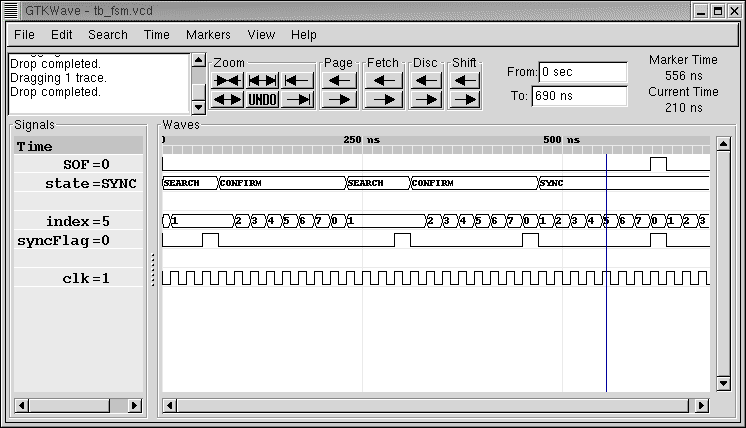
\includegraphics{tbfsm.png}
\fi

Signals are dumped in a suitable format. This format is inferred at
the \class{Signal} construction time, from the type of the initial
value. In particular, \class{bool} signals are dumped as single
bits. (This only works starting with Python~2.3, when \class{bool} has
become a separate type).  Likewise, \class{intbv} signals with a
defined bit width are dumped as bit vectors. To support the general
case, other types of signals are dumped as a string representation, as
returned by the standard \function{str()} function.

\begin{notice}[warning]
Support for literal string representations is not part of the VCD
standard. It is specific to \program{gtkwave}. To generate a
standard VCD file, you need to use signals with a defined bit width
only.
\end{notice}


\section{High level modeling \label{model-hl}}
\index{modeling!high level}

\subsection{Modeling with bus-functional procedures \label{model-bfm}}

\index{bus-functional procedure}%
A \dfn{bus-functional procedure} is a reusable encapsulation of the
low-level operations needed to implement some abstract transaction on
a physical interface. Bus-functional procedures are typically used in
flexible verification environments.

Once again, \myhdl\ uses generator functions to support
bus-functional procedures. In \myhdl\, the difference between
instances and bus-functional procedure calls comes from the way in
which a generator function is used.

As an example, we will design a bus-functional procedure of a
simplified UART transmitter. We assume 8 data bits, no parity bit, and
a single stop bit, and we add print statements to follow the
simulation behavior:

\begin{verbatim}
T_9600 = int(1e9 / 9600)

def rs232_tx(tx, data, duration=T_9600):
    
    """ Simple rs232 transmitter procedure.

    tx -- serial output data
    data -- input data byte to be transmitted
    duration -- transmit bit duration
    
    """

    print "-- Transmitting %s --" % hex(data)
    print "TX: start bit"      
    tx.next = 0
    yield delay(duration)

    for i in range(8):
        print "TX: %s" % data[i]
        tx.next = data[i]
        yield delay(duration)

    print "TX: stop bit"      
    tx.next = 1
    yield delay(duration)
\end{verbatim}

This looks exactly like the generator functions in previous sections. It
becomes a bus-functional procedure when we use it differently. Suppose
that in a test bench, we want to generate a number of data bytes to be
transmitted. This can be modeled as follows:


\begin{verbatim}
testvals = (0xc5, 0x3a, 0x4b)

def stimulus():
    tx = Signal(1)
    for val in testvals:
        txData = intbv(val)
        yield rs232_tx(tx, txData)
\end{verbatim}

We use the bus-functional procedure call as a clause in a
\code{yield} statement. This introduces a fourth form of the
\code{yield} statement: using a generator as a clause. Although this is
a more dynamic usage than in the previous cases, the meaning is
actually very similar: at that point,
the original generator should 
    \index{wait!for the completion of a generator}% 
wait for the completion of a generator. 
In this case, the original generator resumes when the
\code{rs232_tx(tx, txData)} generator returns.

When simulating this, we get:

\begin{verbatim}
-- Transmitting 0xc5 --
TX: start bit
TX: 1
TX: 0
TX: 1
TX: 0
TX: 0
TX: 0
TX: 1
TX: 1
TX: stop bit
-- Transmitting 0x3a --
TX: start bit
TX: 0
TX: 1
TX: 0
TX: 1
...
\end{verbatim}

We will continue with this example by designing the corresponding UART
receiver bus-functional procedure. This will allow us to introduce
further capabilities of \myhdl\ and its use of the \code{yield}
statement. 

Until now, the \code{yield} statements had a single clause. However,
they can have multiple clauses as well. In that case, the generator
resumes as soon as the wait condition specified by one
of the clauses is satisfied. This corresponds to the functionality of
    \index{sensitivity list}%
sensitivity lists in Verilog and VHDL.

For example, suppose we want to design an UART receive procedure with
a timeout. We can specify the timeout condition while waiting for the
start bit, as in the following generator function:

\begin{verbatim}
def rs232_rx(rx, data, duration=T_9600, timeout=MAX_TIMEOUT):
    
    """ Simple rs232 receiver procedure.

    rx -- serial input data
    data -- data received
    duration -- receive bit duration
    
    """

    # wait on start bit until timeout
    yield rx.negedge, delay(timeout)
    if rx == 1:
        raise StopSimulation, "RX time out error"

    # sample in the middle of the bit duration
    yield delay(duration // 2)
    print "RX: start bit"

    for i in range(8):
        yield delay(duration)
        print "RX: %s" % rx
        data[i] = rx

    yield delay(duration)
    print "RX: stop bit"
    print "-- Received %s --" % hex(data)
\end{verbatim}

If the timeout condition is triggered, the receive bit \code{rx}
will still be \code{1}. In that case, we raise an exception to stop
the simulation. The \code{StopSimulation} exception is predefined in
\myhdl\ for such purposes. In the other case, we proceed by
positioning the sample point in the middle of the bit duration, and
sampling the received data bits.

When a \code{yield} statement has multiple clauses, they can be of any
type that is supported as a single clause, including generators. For
example, we can verify the transmitter and receiver generator against
each other by yielding them together, as follows:

\begin{verbatim}
def test():
    tx = Signal(1)
    rx = tx
    rxData = intbv(0)
    for val in testvals:
        txData = intbv(val)
        yield rs232_rx(rx, rxData), rs232_tx(tx, txData)
\end{verbatim}

Both forked generators will run concurrently, and the original
generator will resume as soon as one of them finishes (which will be
the transmitter in this case).  The simulation output shows how
the UART procedures run in lockstep:

\begin{verbatim}
-- Transmitting 0xc5 --
TX: start bit
RX: start bit
TX: 1
RX: 1
TX: 0
RX: 0
TX: 1
RX: 1
TX: 0
RX: 0
TX: 0
RX: 0
TX: 0
RX: 0
TX: 1
RX: 1
TX: 1
RX: 1
TX: stop bit
RX: stop bit
-- Received 0xc5 --
-- Transmitting 0x3a --
TX: start bit
RX: start bit
TX: 0
RX: 0
...
\end{verbatim}

For completeness, we will verify the timeout behavior with a test
bench that disconnects the \code{rx} from the \code{tx} signal, and we
specify a small timeout for the receive procedure:

\begin{verbatim}
def testTimeout():
    tx = Signal(1)
    rx = Signal(1)
    rxData = intbv(0)
    for val in testvals:
        txData = intbv(val)
        yield rs232_rx(rx, rxData, timeout=4*T_9600-1), rs232_tx(tx, txData)
\end{verbatim}
 
The simulation now stops with a timeout exception after a few
transmit cycles:

\begin{verbatim}
-- Transmitting 0xc5 --
TX: start bit
TX: 1
TX: 0
TX: 1
StopSimulation: RX time out error
\end{verbatim}

Recall that the original generator resumes as soon as one of the
forked generators returns. In the previous cases, this is just fine,
as the transmitter and receiver generators run in lockstep. However,
it may be desirable to resume the caller only when \emph{all} of the
forked generators have finished. For example, suppose that we want to
characterize the robustness of the transmitter and receiver design to
bit duration differences. We can adapt our test bench as follows, to
run the transmitter at a faster rate:

\begin{verbatim}
T_10200 = int(1e9 / 10200)

def testNoJoin():
    tx = Signal(1)
    rx = tx
    rxData = intbv(0)
    for val in testvals:
        txData = intbv(val)
        yield rs232_rx(rx, rxData), rs232_tx(tx, txData, duration=T_10200)
\end{verbatim}

Simulating this shows how the transmission of the new byte starts
before the previous one is received, potentially creating additional
transmission errors:

\begin{verbatim}
-- Transmitting 0xc5 --
TX: start bit
RX: start bit
...
TX: 1
RX: 1
TX: 1
TX: stop bit
RX: 1
-- Transmitting 0x3a --
TX: start bit
RX: stop bit
-- Received 0xc5 --
RX: start bit
TX: 0
\end{verbatim}

It is more likely that we want to characterize the design on a byte
by byte basis, and align the two generators before transmitting each
byte. In \myhdl{}, this is done with the \function{join} function. By
joining clauses together in a \code{yield} statement, we create a new
clause that triggers only when all of its clause arguments have
triggered. For example, we can adapt the test bench as follows:

\begin{verbatim}
def testJoin():
    tx = Signal(1)
    rx = tx
    rxData = intbv(0)
    for val in testvals:
        txData = intbv(val)
        yield join(rs232_rx(rx, rxData), rs232_tx(tx, txData, duration=T_10200))
\end{verbatim}

Now, transmission of a new byte only starts when the previous one is received:

\begin{verbatim}
-- Transmitting 0xc5 --
TX: start bit
RX: start bit
...
TX: 1
RX: 1
TX: 1
TX: stop bit
RX: 1
RX: stop bit
-- Received 0xc5 --
-- Transmitting 0x3a --
TX: start bit
RX: start bit
TX: 0
RX: 0
\end{verbatim}



\subsection{Modeling memories with built-in types \label{model-mem}}
\index{modeling!memories}

Python has powerful built-in data types that can be useful to model
hardware memories. This can be merely a matter of putting an interface
around some data type operations.

For example, a \dfn{dictionary} comes in handy to model sparse memory
structures. (In other languages, this data type is called 
\dfn{associative array}, or \dfn{hash table}.) A sparse memory is one in
which only a small part of the addresses is used in a particular
application or simulation. Instead of statically allocating the full
address space, which can be large, it is better to dynamically
allocate the needed storage space. This is exactly what a dictionary
provides. The following is an example of a sparse memory model:

\begin{verbatim}
def sparseMemory(dout, din, addr, we, en, clk):
    
    """ Sparse memory model based on a dictionary.

    Ports:
    dout -- data out
    din -- data in
    addr -- address bus
    we -- write enable: write if 1, read otherwise
    en -- interface enable: enabled if 1
    clk -- clock input
    
    """

    memory = {}

    @always(clk.posedge)
    def access():
        if en:
            if we:
                memory[addr.val] = din.val
            else:
                dout.next = memory[addr.val]

    return access
\end{verbatim} 

Note how we use the \code{val} attribute of the \code{din} signal, as
we don't want to store the signal object itself, but its current
value. Similarly, we use the \code{val} attribute of the \code{addr}
signal as the dictionary key. 

In many cases, \myhdl\ code uses a signal's current value
automatically when there is no ambiguity: for example, when a signal
is used in an expression. However, in other cases such as in this
example you have to refer to the value explicitly: for example, when
the Signal is used as an index, or when it is not used in an
expression.  One option is to use the \code{val} attribute, as in this
example.  Another possibility is to use the \code{int()} or
\code{bool()} functions to typecast the Signal to an integer or a
boolean value. These functions are also useful with \class{intbv}
objects.

As a second example, we will demonstrate how to use a list to model a
synchronous fifo:

\begin{verbatim}
def fifo(dout, din, re, we, empty, full, clk, maxFilling=sys.maxint):
    
    """ Synchronous fifo model based on a list.
    
    Ports:
    dout -- data out
    din -- data in
    re -- read enable
    we -- write enable
    empty -- empty indication flag
    full -- full indication flag
    clk -- clock input

    Optional parameter:
    maxFilling -- maximum fifo filling, "infinite" by default

    """
    
    memory = []

    @always(clk.posedge)
    def access():
        if we:
            memory.insert(0, din.val)
        if re:
            dout.next = memory.pop()
        filling = len(memory)
        empty.next = (filling == 0)
        full.next = (filling == maxFilling)

    return access
\end{verbatim}

Again, the model is merely a \myhdl\ interface around some operations
on a list: \function{insert()} to insert entries, \function{pop()} to
retrieve them, and \function{len()} to get the size of a Python
object.

\subsection{Modeling errors using exceptions \label{model-err}}

In the previous section, we used Python data types for modeling. If
such a type is used inappropriately, Python's run time error system
will come into play. For example, if we access an address in the
\function{sparseMemory} model that was not initialized before, we will
get a traceback similar to the following (some lines omitted for
clarity):

\begin{verbatim}
Traceback (most recent call last):
...
  File "sparseMemory.py", line 31, in access
    dout.next = memory[addr.val]
KeyError: Signal(51)
\end{verbatim}

Similarly, if the \code{fifo} is empty, and we attempt to read from
it, we get:

\begin{verbatim}
Traceback (most recent call last):
...
  File "fifo.py", line 34, in fifo
    dout.next = memory.pop()
IndexError: pop from empty list
\end{verbatim}

Instead of these low level errors, it may be preferable to define
errors at the functional level. In Python, this is typically done by
defining a custom \code{Error} exception, by subclassing the standard
\code{Exception} class. This exception is then raised explicitly when
an error condition occurs.

For example, we can change the \function{sparseMemory} function as
follows (with the doc string is omitted for brevity):

\begin{verbatim}
class Error(Exception):
    pass

def sparseMemory2(dout, din, addr, we, en, clk):
   
    memory = {}

    @always(clk.posedge)
    def access():
        if en:
            if we:
                memory[addr.val] = din.val
            else:
                try:
                    dout.next = memory[addr.val]
                except KeyError:
                    raise Error, "Uninitialized address %s" % hex(addr)

    return access

\end{verbatim}

This works by catching the low level data type exception, and raising
the custom exception with an appropriate error message instead.  If
the \function{sparseMemory} function is defined in a module with the
same name, an access error is now reported as follows:

\begin{verbatim}
Traceback (most recent call last):
...
  File "sparseMemory.py", line 61, in access
    raise Error, "Uninitialized address %s" % hex(addr)
Error: Uninitialized address 0x33

\end{verbatim}

Likewise, the \function{fifo} function can be adapted as follows, to
report underflow and overflow errors:

\begin{verbatim}
class Error(Exception):
    pass


def fifo2(dout, din, re, we, empty, full, clk, maxFilling=sys.maxint):
 
    memory = []

    @always(clk.posedge)
    def access():
        if we:
            memory.insert(0, din.val)
        if re:
            try:
                dout.next = memory.pop()
            except IndexError:
                raise Error, "Underflow -- Read from empty fifo"
        filling = len(memory)
        empty.next = (filling == 0)
        full.next = (filling == maxFilling)
        if filling > maxFilling:
            raise Error, "Overflow -- Max filling %s exceeded" % maxFilling

    return access
\end{verbatim}

In this case, the underflow error is detected as before, by catching a
low level exception on the list data type. On the other hand, the
overflow error is detected by a regular check on the length of the
list.


\subsection{Object oriented modeling \label{model-obj}}
\index{modeling!object oriented}

The models in the previous sections used high-level built-in data
types internally. However, they had a conventional RTL-style
interface.  Communication with such a module is done through signals
that are attached to it during instantiation.

A more advanced approach is to model hardware blocks as
objects. Communication with objects is done through method calls.
A method encapsulates all details of a certain task performed
by the object. As an object has a method interface instead
of an RTL-style hardware interface, this is a much 
higher level approach.

As an example, we will design a synchronized queue object. 
Such an object can be filled by producer, and independently
read by a consumer. When the queue is empty, the consumer
should wait until an item is available. The queue can be modeled
as an object with a \method{put(item)} and a \method{get()}
method, as follows:

\begin{verbatim}
from myhdl import *

def trigger(event):
    event.next = not event

class queue:
    def __init__(self):
       self.l = []
       self.sync = Signal(0)
       self.item = None
    def put(self,item):
       # non time-consuming method
       self.l.append(item)
       trigger(self.sync)
    def get(self):
       # time-consuming method
       if not self.l:
          yield self.sync
       self.item = self.l.pop(0)
\end{verbatim}

The \class{queue} object constructor initializes an internal list to
hold items, and a \var{sync} signal to synchronize the operation
between the methods. Whenever \method{put()} puts an item in the
queue, the signal is triggered.  When the \method{get()} method sees
that the list is empty, it waits on the trigger first.
\method{get()} is a generator method because 
it may consume time. As the \code{yield} statement is used in \myhdl\
for timing control, the method cannot ``yield'' the item. Instead, it
makes it available in the \var{item} instance variable.

To test the queue operation, we will model a producer and a consumer
in the test bench.  As a waiting consumer should not block a whole
system, it should run in a concurrent ``thread''. As always in
\myhdl{}, concurrency is modeled by Python generators. Producer
and consumer will thus run independently, and we will monitor
their operation through some print statements:

\begin{verbatim}
q = queue()

def Producer(q):
    yield delay(120)
    for i in range(5):
        print "%s: PUT item %s" % (now(), i)
        q.put(i)
        yield delay(max(5, 45 - 10*i))

def Consumer(q):
    yield delay(100)
    while 1:
        print "%s: TRY to get item" % now()
        yield q.get()
        print "%s: GOT item %s" % (now(), q.item)
        yield delay(30)

def main():
    P = Producer(q)
    C = Consumer(q)
    return P, C 

sim = Simulation(main())
sim.run()
\end{verbatim}

Note that the generator method \method{get()} is called in a
\code{yield} statement in the \function{Consumer} function. The new
generator will take over from \function{Consumer}, until it is done.
Running this test bench produces the following output:

\begin{verbatim}
% python queue.py
100: TRY to get item
120: PUT item 0
120: GOT item 0
150: TRY to get item
165: PUT item 1
165: GOT item 1
195: TRY to get item
200: PUT item 2
200: GOT item 2
225: PUT item 3
230: TRY to get item
230: GOT item 3
240: PUT item 4
260: TRY to get item
260: GOT item 4
290: TRY to get item
StopSimulation: No more events
\end{verbatim}

\chapter{Unit testing \label{unittest}}

\section{Introduction \label{unittest-intro}}

Many aspects in the design flow of modern digital hardware design can
be viewed as a special kind of software development. From that
viewpoint, it is a natural question whether advances in software
design techniques can not also be applied to hardware design.

One software design approach that gets a lot of attention recently is
\index{extreme programming}%
\emph{Extreme Programming} (XP). It is a fascinating set of techniques and
guidelines that often seems to go against the conventional wisdom. On
other occasions, XP just seems to emphasize the common sense, which
doesn't always coincide with common practice. For example, XP stresses
the importance of normal workweeks, if we are to have the
fresh mind needed for good software development.

It is not my intention nor qualification to present a tutorial on
Extreme Programming. Instead, in this section I will highlight one XP
concept which I think is very relevant to hardware design: the
importance and methodology of unit testing.

\section{The importance of unit tests \label{unittest-why}}

Unit testing is one of the corner stones of Extreme Programming. Other
XP concepts, such as collective ownership of code and continuous
refinement, are only possible by having unit tests. Moreover, XP
emphasizes that writing unit tests should be automated, that they should
test everything in every class, and that they should run perfectly all
the time. 

I believe that these concepts apply directly to hardware design. In
addition, unit tests are a way to manage simulation time. For example,
a state machine that runs very slowly on infrequent events may be
impossible to verify at the system level, even on the fastest
simulator. On the other hand, it may be easy to verify it exhaustively
in a unit test, even on the slowest simulator.

It is clear that unit tests have compelling advantages. On the other
hand, if we need to test everything, we have to write
lots of unit tests. So it should be easy and pleasant
to create, manage and run them. Therefore, XP emphasizes the need for
a unit test framework that supports these tasks. In this chapter,
we will explore the use of the \code{unittest} module from
the standard Python library for creating unit tests for hardware
designs.


\section{Unit test development \label{unittest-dev}}

In this section, we will informally explore the application of unit
test techniques to hardware design. We will do so by a (small)
example: testing a binary to Gray encoder as introduced in
section~\ref{intro-indexing}. 

\subsection{Defining the requirements \label{unittest-req}}

We start by defining the requirements. For a Gray encoder, we want to
the output to comply with Gray code characteristics. Let's define a
\dfn{code} as a list of \dfn{codewords}, where a codeword is a bit
string. A code of order \code{n} has \code{2**n} codewords.

A well-known characteristic is the one that Gray codes are all about:

\newtheorem{reqGray}{Requirement}
\begin{reqGray} 
Consecutive codewords in a Gray code should differ in a single bit.
\end{reqGray}

Is this sufficient? Not quite: suppose for example that an
implementation returns the lsb of each binary input. This would comply
with the requirement, but is obviously not what we want. Also, we don't
want the bit width of Gray codewords to exceed the bit width of the
binary codewords.

\begin{reqGray} 
Each codeword in a Gray code of order n must occur exactly once in the
binary code of the same order.
\end{reqGray}

With the requirements written down we can proceed.

\subsection{Writing the test first \label{unittest-first}}

A fascinating guideline in the XP world is to write the unit test
first. That is, before implementing something, first write the test
that will verify it. This seems to go against our natural inclination,
and certainly against common practices. Many engineers like to
implement first and think about verification afterwards.

But if you think about it, it makes a lot of sense to deal with
verification first. Verification is about the requirements only --- so
your thoughts are not yet cluttered with implementation details. The
unit tests are an executable description of the requirements, so they
will be better understood and it will be very clear what needs to be
done. Consequently, the implementation should go smoother. Perhaps
most importantly, the test is available when you are done
implementing, and can be run anytime by anybody to verify changes.

Python has a standard \code{unittest} module that facilitates writing,
managing and running unit tests. With \code{unittest}, a test case is 
written by creating a class that inherits from
\code{unittest.TestCase}. Individual tests are created by methods of
that class: all method names that start with \code{test} are
considered to be tests of the test case.

We will define a test case for the Gray code properties, and then
write a test for each of the requirements. The outline of the test
case class is as follows:

\begin{verbatim}
from unittest import TestCase

class TestGrayCodeProperties(TestCase):

    def testSingleBitChange(self):
     """ Check that only one bit changes in successive codewords """
     ....


    def testUniqueCodeWords(self):
        """ Check that all codewords occur exactly once """
    ....
\end{verbatim}

Each method will be a small test bench that tests a single
requirement. To write the tests, we don't need an implementation of
the Gray encoder, but we do need the interface of the design. We can
specify this by a dummy implementation, as follows:

\begin{verbatim}
def bin2gray(B, G, width):
    ### NOT IMPLEMENTED YET! ###
    yield None
\end{verbatim}

For the first requirement, we will write a test bench that applies all
consecutive input numbers, and compares the current output with the
previous one for each input. Then we check that the difference is a
single bit. We will test all Gray codes up to a certain order
\code{MAX_WIDTH}.

\begin{verbatim}
    def testSingleBitChange(self):
        """ Check that only one bit changes in successive codewords """
        
        def test(B, G, width):
            B.next = intbv(0)
            yield delay(10)
            for i in range(1, 2**width):
                G_Z.next = G
                B.next = intbv(i)
                yield delay(10)
                diffcode = bin(G ^ G_Z)
                self.assertEqual(diffcode.count('1'), 1)
        
        for width in range(1, MAX_WIDTH):
            B = Signal(intbv(-1))
            G = Signal(intbv(0))
            G_Z = Signal(intbv(0))
            dut = bin2gray(B, G, width)
            check = test(B, G, width)
            sim = Simulation(dut, check)
            sim.run(quiet=1)
\end{verbatim}

Note how the actual check is performed by a \code{self.assertEqual}
method, defined by the \code{unittest.TestCase} class.

Similarly, we write a test bench for the second requirement. Again, we
simulate all numbers, and put the result in a list. The requirement
implies that if we sort the result list, we should get a range of
numbers:

\begin{verbatim}
    def testUniqueCodeWords(self):
        """ Check that all codewords occur exactly once """

        def test(B, G, width):
            actual = []
            for i in range(2**width):
                B.next = intbv(i)
                yield delay(10)
                actual.append(int(G))
            actual.sort()
            expected = range(2**width)
            self.assertEqual(actual, expected)
       
        for width in range(1, MAX_WIDTH):
            B = Signal(intbv(-1))
            G = Signal(intbv(0))
            dut = bin2gray(B, G, width)
            check = test(B, G, width)
            sim = Simulation(dut, check)
            sim.run(quiet=1)
\end{verbatim}


\subsection{Test-driven implementation \label{unittest-impl}}

With the test written, we begin with the implementation. For
illustration purposes, we will intentionally write some incorrect
implementations to see how the test behaves.

The easiest way to run tests defined with the \code{unittest}
framework, is to put a call to its \code{main} method at the end of
the test module:

\begin{verbatim}
unittest.main()
\end{verbatim}

Let's run the test using the dummy Gray encoder shown earlier:

\begin{verbatim}
% python test_gray.py -v
Check that only one bit changes in successive codewords ... FAIL
Check that all codewords occur exactly once ... FAIL
<trace backs not shown>
\end{verbatim}

As expected, this fails completely. Let us try an incorrect
implementation, that puts the lsb of in the input on the output:

\begin{verbatim}
def bin2gray(B, G, width):
    ### INCORRECT - DEMO PURPOSE ONLY! ###

    @always_comb
    def logic():
        G.next = B[0]

    return logic
\end{verbatim}


Running the test produces:

\begin{verbatim}
% python test_gray.py -v
Check that only one bit changes in successive codewords ... ok
Check that all codewords occur exactly once ... FAIL

======================================================================
FAIL: Check that all codewords occur exactly once
----------------------------------------------------------------------
Traceback (most recent call last):
  File "test_gray.py", line 109, in testUniqueCodeWords
    sim.run(quiet=1)
...
  File "test_gray.py", line 104, in test
    self.assertEqual(actual, expected)
  File "/usr/local/lib/python2.2/unittest.py", line 286, in failUnlessEqual
    raise self.failureException, \
AssertionError: [0, 0, 1, 1] != [0, 1, 2, 3]

----------------------------------------------------------------------
Ran 2 tests in 0.785s
\end{verbatim}

Now the test passes the first requirement, as expected, but fails the
second one. After the test feedback, a full traceback is shown that
can help to debug the test output.

Finally, if we use the correct implementation as in
section~\ref{intro-indexing}, the output is:

\begin{verbatim}
% python test_gray.py -v
Check that only one bit changes in successive codewords ... ok
Check that all codewords occur exactly once ... ok

----------------------------------------------------------------------
Ran 2 tests in 6.364s

OK
\end{verbatim}



\subsection{Changing requirements \label{unittest-change}}

In the previous section, we concentrated on the general requirements
of a Gray code. It is possible to specify these without specifying the
actual code. It is easy to see that there are several codes
that satisfy these requirements. In good XP style, we only tested
the requirements and nothing more.

It may be that more control is needed. For example, the requirement
may be for a particular code, instead of compliance with general
properties. As an illustration, we will show how to test for
\emph{the} original Gray code, which is one specific instance that
satisfies the requirements of the previous section. In this particular
case, this test will actually be easier than the previous one.

We denote the original Gray code of order \code{n} as \code{Ln}. Some
examples: 

\begin{verbatim}
L1 = ['0', '1']
L2 = ['00', '01', '11', '10']
L3 = ['000', '001', '011', '010', '110', '111', '101', 100']
\end{verbatim}

It is possible to specify these codes by a recursive algorithm, as
follows:

\begin{enumerate}
\item L1 = ['0', '1']
\item Ln+1 can be obtained from Ln as follows. Create a new code Ln0 by
prefixing all codewords of Ln with '0'. Create another new code Ln1 by
prefixing all codewords of Ln with '1', and reversing their
order. Ln+1 is the concatenation of Ln0 and Ln1.
\end{enumerate}

Python is well-known for its elegant algorithmic
descriptions, and this is a good example. We can write the algorithm
in Python as follows:

\begin{verbatim}
def nextLn(Ln):
    """ Return Gray code Ln+1, given Ln. """
    Ln0 = ['0' + codeword for codeword in Ln]
    Ln1 = ['1' + codeword for codeword in Ln]
    Ln1.reverse()
    return Ln0 + Ln1
\end{verbatim}

The code \samp{['0' + codeword for ...]} is called a \dfn{list
comprehension}. It is a concise way to describe lists built by short
computations in a for loop.

The requirement is now that the output code matches the
expected code Ln. We use the \code{nextLn} function to compute the
expected result. The new test case code is as follows:

\begin{verbatim}
class TestOriginalGrayCode(TestCase):

    def testOriginalGrayCode(self):
        """ Check that the code is an original Gray code """

        Rn = []
        
        def stimulus(B, G, n):
            for i in range(2**n):
                B.next = intbv(i)
                yield delay(10)
                Rn.append(bin(G, width=n))
        
        Ln = ['0', '1'] # n == 1
        for n in range(2, MAX_WIDTH):
            Ln = nextLn(Ln)
            del Rn[:]
            B = Signal(intbv(-1))
            G = Signal(intbv(0))
            dut = bin2gray(B, G, n)
            stim = stimulus(B, G, n)
            sim = Simulation(dut, stim)
            sim.run(quiet=1)
            self.assertEqual(Ln, Rn)
\end{verbatim}

As it happens, our implementation is apparently an original Gray code:

\begin{verbatim}
% python test_gray.py -v TestOriginalGrayCode
Check that the code is an original Gray code ... ok

----------------------------------------------------------------------
Ran 1 tests in 3.091s

OK
\end{verbatim}


 


\chapter{Co-simulation with Verilog and VHDL \label{cosim}}

\section{Introduction \label{cosim-intro}}

One of the most exciting possibilities of \myhdl\
is to use it as a hardware verification language (HVL).
A HVL is a language used to write test benches and
verification environments, and to control simulations.

Nowadays, it is generally acknowledged that HVLs should be equipped
with modern software techniques, such as object orientation. The
reason is that verification it the most complex and time-consuming
task of the design process. Consequently, every useful technique is
welcome. Moreover, test benches are not required to be
implementable. Therefore, unlike with synthesizable code, there
are no constraints on creativity.

Technically, verification of a design implemented in
another language requires co-simulation. \myhdl\ is 
enabled for co-simulation with any HDL simulator that
has a procedural language interface (PLI). The \myhdl\
side is designed to be independent of a particular
simulator, On the other hand, for each HDL simulator a specific
PLI module will have to be written in C. Currently,
the \myhdl\ release contains a PLI module for
two Verilog simulators: Icarus and Cver.

\section{The HDL side \label{cosim-hdl}}

To introduce co-simulation, we will continue to use the Gray encoder
example from the previous chapters. Suppose that we want to
synthesize it and write it in Verilog for that purpose. Clearly we would
like to reuse our unit test verification environment. 

To start, let's recall how the Gray encoder in \myhdl{} looks like:

\begin{verbatim}
def bin2gray(B, G, width):
    """ Gray encoder.

    B -- input intbv signal, binary encoded
    G -- output intbv signal, gray encoded
    width -- bit width
    """

    @always_comb
    def logic():
        for i in range(width):
            G.next[i] = B[i+1] ^ B[i]

    return logic
\end{verbatim}

To show the co-simulation flow, we don't need the Verilog
implementation yet, but only the interface.  Our Gray encoder in
Verilog would have the following interface:

\begin{verbatim}
module bin2gray(B, G);

   parameter width = 8;
   input [width-1:0]  B;     
   output [width-1:0] G;
   ....
\end{verbatim}

To write a test bench, one creates a new module that instantiates the
design under test (DUT).  The test bench declares nets and
regs (or signals in VHDL) that are attached to the DUT, and to
stimulus generators and response checkers. In an all-HDL flow, the
generators and checkers are written in the HDL itself, but we will
want to write them in \myhdl{}. To make the connection, we need to
declare which regs \& nets are driven and read by the \myhdl\
simulator. For our example, this is done as follows:

\begin{verbatim}
module dut_bin2gray;

   reg [`width-1:0] B;
   wire [`width-1:0] G;

   initial begin
      $from_myhdl(B);
      $to_myhdl(G);
   end

   bin2gray dut (.B(B), .G(G));
   defparam dut.width = `width;

endmodule
\end{verbatim}

The \code{\$from_myhdl} task call declares which regs are driven by
\myhdl{}, and the \code{\$to_myhdl} task call which regs \& nets are read
by it. These tasks take an arbitrary number of arguments.  They are
defined in a PLI module written in C and made available in a
simulator-dependent manner.  In Icarus Verilog, the tasks are defined
in a \code{myhdl.vpi} module that is compiled from C source code.

\section{The \myhdl\ side \label{cosim-myhdl}}

\myhdl\ supports co-simulation by a \code{Cosimulation} object. 
A \code{Cosimulation} object must know how to run a HDL simulation.
Therefore, the first argument to its constructor is a command string
to execute a simulation.

The way to generate and run an simulation executable is simulator
dependent.  For example, in Icarus Verilog, a simulation executable
for our example can be obtained obtained by running the
\code{iverilog} compiler as follows:

\begin{verbatim}
% iverilog -o bin2gray -Dwidth=4 bin2gray.v dut_bin2gray.v
\end{verbatim}

This generates a \code{bin2gray} executable for a parameter \code{width}
of 4, by compiling the contributing verilog files.

The simulation itself is run by the \code{vvp} command:

\begin{verbatim}
% vvp -m ./myhdl.vpi bin2gray
\end{verbatim}

This runs the \code{bin2gray} simulation, and specifies to use the
\code{myhdl.vpi} PLI module present in the current directory. (This is 
just a command line usage example; actually simulating with the
\code{myhdl.vpi} module is only meaningful from a
\code{Cosimulation} object.)

We can use a \code{Cosimulation} object to provide a HDL
version of a design to the \myhdl\ simulator. Instead of a generator
function, we write a function that returns a \code{Cosimulation}
object. For our example and the Icarus Verilog simulator, this is done
as follows:

\begin{verbatim}
import os

from myhdl import Cosimulation

cmd = "iverilog -o bin2gray -Dwidth=%s bin2gray.v dut_bin2gray.v"
      
def bin2gray(B, G, width):
    os.system(cmd % width)
    return Cosimulation("vvp -m ./myhdl.vpi bin2gray", B=B, G=G)
\end{verbatim}

After the executable command argument, the \code{Cosimulation}
constructor takes an arbitrary number of keyword arguments. Those
arguments make the link between \myhdl\ Signals and HDL nets, regs, or
signals, by named association. The keyword is the name of an argument
in a \code{\$to_myhdl} or \code{\$from_myhdl} call; the argument is
a \myhdl\ Signal.

With all this in place, we can now use the existing unit test
to verify the Verilog implementation. Note that we kept the
same name and parameters for the the \code{bin2gray} function:
all we need to do is to provide this alternative definition
to the existing unit test.

Let's try it on the Verilog design:

\begin{verbatim}
module bin2gray(B, G);

   parameter width = 8;
   input [width-1:0]  B;
   output [width-1:0] G;
   reg [width-1:0] G;
   integer i;
   wire [width:0] extB;

   assign extB = {1'b0, B}; // zero-extend input

   always @(extB) begin
      for (i=0; i < width; i=i+1)
        G[i] <= extB[i+1] ^ extB[i];
   end

endmodule
\end{verbatim}

When we run our unit test, we get:

\begin{verbatim}
% python test_bin2gray.py 
Check that only one bit changes in successive codewords ... ok
Check that all codewords occur exactly once ... ok
Check that the code is an original Gray code ... ok

----------------------------------------------------------------------
Ran 3 tests in 2.729s

OK
\end{verbatim}


\section{Restrictions \label{cosim-restr}}

In the ideal case, it should be possible to simulate
any HDL description seamlessly with \myhdl{}. Moreover
the communicating signals at each side should act
transparently as a single one, enabling fully race free
operation.

For various reasons, it may not be possible or desirable
to achieve full generality. As anyone that has developed
applications with the Verilog PLI can testify, the
restrictions in a particular simulator, and the 
differences over various simulators, can be quite 
frustrating. Moreover, full generality may require
a disproportionate amount of development work compared
to a slightly less general solution that may
be sufficient for the target application.

Consequently, I have tried to achieve a solution
which is simple enough so that one can reasonably 
expect that any PLI-enabled simulator can support it,
and that is relatively easy to verify and maintain.
At the same time, the solution is sufficiently general 
to cover the target application space.

The result is a compromise that places certain restrictions
on the HDL code. In this section, these restrictions 
are presented.

\subsection{Only passive HDL can be co-simulated \label{cosim-pass}}

The most important restriction of the \myhdl\ co-simulation solution is
that only ``passive'' HDL can be co-simulated.  This means that the HDL
code should not contain any statements with time delays. In other
words, the \myhdl\ simulator should be the master of time; in
particular, any clock signal should be generated at the \myhdl\ side.

At first this may seem like an important restriction, but if one
considers the target application for co-simulation, it probably
isn't. 

\myhdl\ supports co-simulation so that test benches for HDL
designs can be written in Python.  Let's consider the nature of the
target HDL designs. For high-level, behavioral models that are not
intended for implementation, it should come as no surprise that I
would recommend to write them in \myhdl\ directly; that is one of the
goals of the \myhdl\ effort. Likewise, gate level designs with
annotated timing are not the target application: static timing
analysis is a much better verification method for such designs.

Rather, the targeted HDL designs are naturally models that are
intended for implementation, most likely through synthesis. As time
delays are meaningless in synthesizable code, the restriction is
compatible with the target application.

\subsection{Race sensitivity issues \label{cosim-race}}

In a typical RTL code, some events cause other events to occur in the
same time step. For example, when a clock signal triggers some signals
may change in the same time step. For race-free operation, an HDL
must differentiate between such events within a time step. This is done
by the concept of ``delta'' cycles. In a fully general, race free
co-simulation, the co-simulators would communicate at the level of delta
cycles. However, in \myhdl\ co-simulation, this is not entirely the
case.

Delta cycles from the \myhdl\ simulator toward the HDL co-simulator are
preserved. However, in the opposite direction, they are not. The
signals changes are only returned to the \myhdl\ simulator after all delta
cycles have been performed in the HDL co-simulator.

What does this mean? Let's start with the good news. As explained in
the previous section, the concept behind \myhdl\ co-simulation implies
that clocks are generated at the \myhdl\ side.  \emph{When using a
\myhdl\ clock and its corresponding HDL signal directly as a clock,
co-simulation is race free.} In other words, the case
that most closely reflects the \myhdl\ co-simulation approach, is race free.

The situation is different when you want to use a signal driven by the
HDL (and the corresponding MyHDL signal) as a clock. 
Communication triggered by such a clock is not race free. The solution
is to treat such an interface as a chip interface instead of an RTL
interface.  For example, when data is triggered at positive clock
edges, it can safely be sampled at negative clock edges.
Alternatively, the \myhdl\ data signals can be declared with a delay
value, so that they are guaranteed to change after the clock
edge.


\section{Implementation notes \label{cosim-impl}}

\begin{quote}
\em
This section requires some knowledge of PLI terminology.
\end{quote}

Enabling a simulator for co-simulation requires a PLI module written
in C. In Verilog, the PLI is part of the ``standard''.  However,
different simulators implement different versions and portions of the
standard. Worse yet, the behavior of certain PLI callbacks is not
defined on some essential points.  As a result, one should plan to
write or at least customize a specific PLI module for any simulator.
The release contains a PLI module for the open source Icarus
and Cver simulators. 

This section documents the current approach and status of the PLI
module implementation and some reflections on future
implementations.

\subsection{Icarus Verilog \label{cosim-icarus}}

\subsubsection{Delta cycle implementation \label{cosim-icarus-delta}}

To make co-simulation work, a specific type of PLI callback is
needed. The callback should be run when all pending events have been
processed, while allowing the creation of new events in the current
time step (e.g. by the \myhdl\ simulator).  In some Verilog
simulators, the \code{cbReadWriteSync} callback does exactly
that. However, in others, including Icarus, it does not. The
callback's behavior is not fully standardized; some simulators run the
callback before non-blocking assignment events have been processed.

Consequently, I had to look for a workaround. One half of the solution
is to use the \code{cbReadOnlySync} callback.  This callback runs
after all pending events have been processed.  However, it does not
permit to create new events in the current time step.  The second half
of the solution is to map \myhdl\ delta cycles onto real Verilog time
steps.  Note that fortunately I had some freedom here because of the
restriction that only passive HDL code can be co-simulated.

I chose to make the time granularity in the Verilog simulator a 1000
times finer than in the \myhdl{} simulator. For each \myhdl\ time
step, 1000 Verilog time steps are available for \myhdl\ delta
cycles. In practice, only a few delta cycles per time step should be
needed. Exceeding this limit almost certainly indicates a design error;
the limit is checked at run-time. The factor 1000 also makes it
easy to distinguish ``real'' time from delta cycle time when printing
out the Verilog time.

\subsubsection{Passive Verilog check \label{cosim-icarus-pass}}

As explained before, co-simulated Verilog should not contain delay
statements. Ideally, there should be a run-time check to flag
non-compliant code. However, there is currently no such check in the
Icarus module.

The check can be written using the \code{cbNextSimTime} VPI callback
in Verilog. However, Icarus 0.7 doesn't support this callback. In the
meantime, support for it has been added to the Icarus development
branch.  When Icarus 0.8 is released, a check will be added.

In the mean time, just don't do this. It may appear to ``work'' but it
really won't as events will be missed over the co-simulation
interface.


\subsection{Cver \label{cosim-cver}}

MyHDL co-simulation is supported with the open source Verilog
simulator Cver. The PLI module is based on the one for Icarus
and basically has the same functionality. Only some cosmetic
modifications were required.

\subsection{Other Verilog simulators \label{cosim-impl-verilog}}

The Icarus module is written with VPI calls, which are provided by the
most recent generation of the Verilog PLI. Some simulators may only
support TF/ACC calls, requiring a complete redesign of the interface
module.

If the simulator supports VPI, the Icarus module should be reusable to
a large extent. However, it may be possible to improve on it.  The
workaround to support delta cycles described in
Section~\ref{cosim-icarus-delta} may not be necessary. In some
simulators, the \code{cbReadWriteSync} callback occurs after all
events (including non-blocking assignments) have been processed. In
that case, the functionality can be supported without a finer time
granularity in the Verilog simulator.

There are also Verilog standardization efforts underway to resolve the
ambiguity of the \code{cbReadWriteSync} callback. The solution will be
to introduce new, well defined callbacks. From reading some proposals,
I conclude that the \code{cbEndOfSimTime} callback would provide the
required functionality.

The MyHDL project currently has no access to commercial Verilog
simulators, so progress in co-simulation support depends on external
interest and participation. Users have reported that they are using
MyHDL co-simulation with the simulators from Aldec and Modelsim.


\subsection{Interrupted system calls \label{cosim-impl-syscalls}}

The PLI module uses \code{read} and \code{write} system calls to
communicate between the co-simulators. The implementation assumes that
these calls are restarted automatically by the operating system when
interrupted. This is apparently what happens on the Linux box on which
MyHDL is developed.

It is known how non-restarted interrupted system calls should be
handled, but currently such code cannot be tested on the MyHDL
development platform. Also, it is not clear whether this is still a
relevant issue with modern operating systems. Therefore, this issue
has not been addressed at this moment. However, assertions have been
included that should trigger when this situation occurs.

Whenever an assertion fires in the PLI module, please report it.  The
same holds for Python exceptions that cannot be easily explained.

\subsection{VHDL \label{cosim-impl-vhdl}}

It would be nice to have an interface to VHDL simulators such as the
Modelsim VHDL simulator. This will require a PLI module using the
PLI of the VHDL simulator. 

The MyHDL project currently has no access to commercial VHDL
simulators, so progress in co-simulation support will depend on
external interest and participation.


\chapter{Conversion to Verilog\label{conv}}
\section{Introduction\label{conv-intro}}

\myhdl\ supports the automatic conversion of implementation-oriented
\myhdl\ code to Verilog code. This feature provides a
direct path from Python to an FPGA or ASIC implementation.

\section{Solution description\label{conv-solution}}

The solution works as follows. The hardware description should
satisfy certain constraints that are typical for
implementation-oriented hardware modeling.  Subsequently, such a
design is converted to an equivalent model in the Verilog language,
using the function \function{toVerilog} from the \myhdl\
library. Finally, a third-party \emph{synthesis tool} is used to
convert the Verilog design to a gate implementation for an ASIC or
FPGA. There are a number of Verilog synthesis tools available, varying
in price, capabilities, and target implementation technology.

The conversion does not start from source files, but from an
instantiated design that has been \emph{elaborated} by the Python
interpreter. The converter uses the Python profiler to track the
interpreter's operation and to infer the design structure and name
spaces. It then selectively compiles pieces of source code for
additional analysis and for conversion. This is done using the Python
compiler package.

\section{Features\label{conv-features}}

\subsection{The design is converted after elaboration\label{conv-features-elab}}
\emph{Elaboration} refers to the initial processing of a hardware
description to achieve a representation of a design instance that is
ready for simulation or synthesis. In particular, structural
parameters and constructs are processed in this step. In \myhdl{}, the
Python interpreter itself is used for elaboration.  A
\class{Simulation} object is constructed with elaborated design
instances as arguments.  Likewise, the Verilog conversion works on an
elaborated design instance. The Python interpreter is thus used as
much as possible.

\subsection{The structural description can be arbitrarily complex and hierarchical\label{conv-features-struc}}
As the conversion works on an elaborated design instance, any modeling
constraints only apply to the leaf elements of the design structure,
that is, the co-operating generators. In other words, there are no
restrictions on the description of the design structure: Python's full
power can be used for that purpose. Also, the design hierarchy can be
arbitrarily deep.

\subsection{Generators are mapped to Verilog always or initial blocks\label{conv-features-gen}}
The converter analyzes the code of each generator and maps it
to a Verilog \code{always} blocks if possible, and to 
an \code{initial} block otherwise.
The converted Verilog design will be a flat
"net list of blocks".

\subsection{The Verilog module interface is inferred from signal usage\label{conv-features-intf}}
In \myhdl{}, the input or output direction of interface signals
is not explicitly declared. The converter investigates signal usage
in the design hierarchy to infer whether a signal is used as
input, output, or as an internal signal. Internal signals are
given a hierarchical name in the Verilog output.

\subsection{Function calls are mapped to a unique Verilog function or task call\label{conv-features-func}}
The converter analyzes function calls and function code to see if they
should be mapped to Verilog functions or to tasks. Python functions
are much more powerful than Verilog subprograms; for example, they are
inherently generic, and they can be called with named association.  To
support this power in Verilog, a unique Verilog function or task is
generated per Python function call.

\subsection{If-then-else structures may be mapped to Verilog case statements\label{conv-features-if}}
Python does not provide a case statement. However, 
the converter recognizes if-then-else structures in which a variable is
sequentially compared to items of an enumeration type, and maps
such a structure to a Verilog case statement with the appropriate
synthesis attributes.

\subsection{Choice of encoding schemes for enumeration types\label{conv-features-enum}}
The \function{enum} function in \myhdl\ returns an enumeration type. This
function takes an additional parameter \var{encoding} that specifies the
desired encoding in the implementation: binary, one hot, or one cold.
The Verilog converter generates the appropriate code.

\subsection{Support for RAM inference \label{conf-features-ram}}
Certain synthesis tools can map Verilog memories to RAM
structures. To support this interesting feature, the Verilog converter
maps lists of signals to Verilog memories.

\subsection{Support for ROM memory \label{conf-features-rom}}
Some synthesis tools can infer a ROM
from a case statement. The Verilog converter does the expansion into
a case statement automatically, based on a higher level
description. The ROM access is described in a single line, by
indexing into a tuple of integers.

\subsection{Support for signed arithmetic \label{conf-features-signed}}
In MyHDL, working with negative numbers is trivial: one just uses
\code{intbv} objects with negative values.
By contrast, negative numbers are tricky in Verilog. The language
makes a difference between an unsigned and a signed representation,
and the user has to declare signed variables explicitly.  When the two
representations are mixed in an expression, all operands are
interpreted as unsigned, which typically leads to unexpected results.

The Verilog converter handles negative \code{intbv} objects by using
a signed Verilog representation. Also, it automatically performs sign
extension and casting to a signed representation when unsigned numbers
are used in a mixed expression. In this way, it automates a task which
is notoriously hard to get right in Verilog directly.

\subsection{Support for user-defined Verilog code \label{conf-features-udfv}}
If desired, the user can bypass the regular Verilog conversion
and describe user-defined code to be inserted instead.

\section{The convertible subset\label{conv-subset}}

\subsection{Introduction\label{conv-subset-intro}}

Unsurprisingly, not all \myhdl\ code can be converted to Verilog. In
fact, there are very important restrictions.  As the goal of the
conversion functionality is implementation, this should not be a big
issue: anyone familiar with synthesis is used to similar restrictions
in the \emph{synthesizable subset} of Verilog and VHDL. The converter
attempts to issue clear error messages when it encounters a construct
that cannot be converted. 

In practice, the synthesizable subset usually refers to RTL synthesis,
which is by far the most popular type of synthesis today. There are
industry standards that define the RTL synthesis subset.  However,
those were not used as a model for the restrictions of the MyHDL
converter, but as a minimal starting point.  On that basis, whenever
it was judged easy or useful to support an additional feature, this
was done. For example, it is actually easier to convert
\keyword{while} loops than \keyword{for} loops even though they are
not RTL-synthesizable.  As another example, \keyword{print} is
supported because it's so useful for debugging, even though it's not
synthesizable.  In summary, the convertible subset is a superset of
the standard RTL synthesis subset, and supports synthesis tools with
more advanced capabilities, such as behavioral synthesis.

Recall that any restrictions only apply to the design post
elaboration.  In practice, this means that they apply only to the code
of the generators, that are the leaf functional blocks in a MyHDL
design.

\subsection{Coding style\label{conv-subset-style}}

A natural restriction on convertible code is that it should be
written in MyHDL style: cooperating generators, communicating through
signals, and with sensitivity lists specifying wait points and resume
conditions.  Supported resume conditions are a signal edge, a signal
change, or a tuple of such conditions.

\subsection{Supported types\label{conv-subset-types}}

The most important restriction regards object types. Verilog is an
almost typeless language, while Python is strongly (albeit
dynamically) typed. The converter has to infer the types of names
used in the code, and map those names to Verilog variables.

Only a limited amount of types can be converted.
Python \class{int} and \class{long} objects are mapped to Verilog
integers. All other supported types are mapped to Verilog regs (or
wires), and therefore need to have a defined bit width. The supported
types are the Python \class{bool} type, the MyHDL \class{intbv} type,
and MyHDL enumeration types returned by function \function{enum}. The
latter objects can also be used as the base object of a
\class{Signal}. 

\class{intbv} objects must be constructed so that a bit
width can be inferred. This can be done by specifying minimum
and maximum values, e.g. as follows:

\begin{verbatim}
index = intbv(0, min=MIN, max=MAX)
\end{verbatim}

The Verilog converter supports \class{intbv} objects that
can take negative values.

Alternatively, a slice can be taken from an \class{intbv} object
as follows:

\begin{verbatim}
index = intbv(0)[N:]
\end{verbatim}

Such as slice returns a new \class{intbv} object, with minimum
value \code{0} , and maximum value \code{2**N}.


\subsection{Supported statements\label{conv-subset-statements}}

The following is a list of the statements that are supported by the
Verilog converter, possibly qualified with restrictions
or usage notes. 

\begin{description}

\item[\keyword{break}]

\item[\keyword{continue}]

\item[\keyword{def}]

\item[\keyword{for}]
The only supported iteration scheme is iterating through sequences of
integers returned by built-in function \function{range} or \myhdl\
function \function{downrange}.  The optional \keyword{else} clause is
not supported.

\item[\keyword{if}]
\keyword{if}, \keyword{elif}, and \keyword{else} clauses
are fully supported.

\item[\keyword{pass}]

\item[\keyword{print}]
When printing an interpolated string, the format specifiers are copied
verbatim to the Verilog output.  Printing to a file (with syntax
\code{'>>'}) is not supported.

\item[\keyword{raise}]
This statement is mapped to Verilog statements
that end the simulation with an error message.

\item[\keyword{return}]

\item[\keyword{yield}] 
The yielded expression can be a signal, a signal edge
as specified by \myhdl\ functions \function{posedge}
or \function{negedge}, or a tuple of signals and
edge specifications.

\item[\keyword{while}]
The optional \keyword{else}
clause is not supported.

\end{description}

\subsection{Supported built-in functions\label{conv-subset-builtin}}

The following is a list of the built-in functions that are supported by the
Verilog converter.

\begin{description}
\item[\function{bool()}]
This function can be used to typecast an object explictly to
its boolean interpretation.

\item[\function{len()}]
For \class{Signal} and \class{intbv} objects, function \function{len()}
returns the bit width.

\item[\function{int()}]
This function can be used to typecast an object explictly to
its integer interpretation.

\end{description}

\subsection{Excluding code from conversion \label{conv-subset-exclude}}
For some tasks, such as debugging, it may be useful to insert arbitratry
Python code that should not be converted.

The Verilog convertor supports this by ignoring all code that is
embedded in a \code{if __debug__} test. The value of the
\code{__debug__} variable is not taken into account.

\section{Methodology notes\label{conv-meth}}

\subsection{Simulation\label{conv-meth-sim}}

In the Python philosophy, the run-time rules. The Python compiler
doesn't attempt to detect a lot of errors beyond syntax errors, which
given Python's ultra-dynamic nature would be an almost impossible task
anyway. To verify a Python program, one should run it, preferably
using unit testing to verify each feature.

The same philosophy should be used when converting a MyHDL description
to Verilog: make sure the simulation runs fine first. Although the
converter checks many things and attempts to issue clear error
messages, there is no guarantee that it does a meaningful job unless
the simulation runs fine.

\subsection{Conversion output verification\label{conv-meth-conv}}
It is always prudent to verify the converted Verilog output.
To make this task easier, the converter also generates a
test bench that makes it possible to simulate the Verilog
design using the Verilog co-simulation interface. This 
permits to verify the Verilog code with the same test
bench used for the \myhdl\ code. This is also how
the Verilog converter development is being verified.

\subsection{Assignment issues\label{conv-meth-assign}}

\subsubsection{Name assignment in Python\label{conv-meth-assign-python}}

Name assignment in Python is a different concept than in
many other languages. This point is very important for
effective modeling in Python, and even more so
for synthesizable \myhdl\ code. Therefore, the issues are
discussed here explicitly.

Consider the following name assignments:

\begin{verbatim}
a = 4
a = ``a string''
a = False
\end{verbatim}

In many languages, the meaning would be that an
existing variable \var{a} gets a number of different values.
In Python, such a concept of a variable doesn't exist. Instead,
assignment merely creates a new binding of a name to a
certain object, that replaces any previous binding.
So in the example, the name \var{a} is bound a 
number of different objects in sequence.

The Verilog converter has to investigate name
assignment and usage in \myhdl\ code, and to map
names to Verilog variables. To achieve that,
it tries to infer the type and possibly the
bit width of each expression that is assigned
to a name.

Multiple assignments to the same name can be supported if it can be
determined that a consistent type and bit width is being used in the
assignments. This can be done for boolean expressions, numeric
expressions, and enumeration type literals. In Verilog, the
corresponding name is mapped to a single bit \code{reg}, an
\code{integer}, or a \code{reg} with the appropriate width, respectively.

In other cases, a single assignment should be used when an object is
created. Subsequent value changes are then achieved by modification of
an existing object.  This technique should be used for \class{Signal}
and \class{intbv} objects.

\subsubsection{Signal assignment\label{conv-meth-assign-signal}}

Signal assignment in \myhdl\ is implemented using attribute assignment
to attribute \code{next}.  Value changes are thus modeled by
modification of the existing object. The converter investigates the
\class{Signal} object to infer the type and bit width of the
corresponding Verilog variable.

\subsubsection{\class{intbv} objects\label{conv-meth-assign-intbv}}

Type \class{intbv} is likely to be the workhorse for synthesizable
modeling in \myhdl{}. An \class{intbv} instance behaves like a
(mutable) integer whose individual bits can be accessed and
modified. Also, it is possible to constrain its set of values. In
addition to error checking, this makes it possible to infer a bit
width, which is required for implementation.

In Verilog, an \class{intbv} instance will be mapped to a \code{reg}
with an appropriate width. As noted before, it is not possible
to modify its value using name assignment. In the following, we
will show how it can be done instead. Consider:

\begin{verbatim}
a = intbv(0)[8:]
\end{verbatim}

This is an \class{intbv} object with initial value \code{0} and
bit width 8. The change its value to \code{5}, we can use
slice assignment:

\begin{verbatim}
a[8:] = 5
\end{verbatim}

The same can be achieved by leaving the bit width unspecified, 
which has the meaning to change ``all'' bits:

\begin{verbatim}
a[:] = 5
\end{verbatim}

Often the new value will depend on the old one. For example,
to increment an \class{intbv} with the technique above:

\begin{verbatim}
a[:] = a + 1
\end{verbatim}

Python also provides \emph{augmented} assignment operators,
which can be used to implement in-place operations. These are supported
on \class{intbv} objects and by the converter, so that the increment
can also be done as follows:

\begin{verbatim}
a += 1
\end{verbatim}

\section{Converter usage\label{conv-usage}}

We will demonstrate the conversion process by showing some examples.

\subsection{A small sequential design\label{conv-usage-seq}}

Consider the following MyHDL code for an incrementer module:

\begin{verbatim}
ACTIVE_LOW, INACTIVE_HIGH = 0, 1

def inc(count, enable, clock, reset, n):
    
    """ Incrementer with enable.
    
    count -- output
    enable -- control input, increment when 1
    clock -- clock input
    reset -- asynchronous reset input
    n -- counter max value
    
    """
    
    @always(clock.posedge, reset.negedge)
    def incProcess():
        if reset == ACTIVE_LOW:
            count.next = 0
        else:
            if enable:
                count.next = (count + 1) % n
                
    return incProcess
\end{verbatim}

In Verilog terminology, function \function{inc} corresponds to a
module, while the decorated function \function{incProcess}
roughly corresponds to an always block.

Normally, to simulate the design, we would "elaborate" an instance
as follows:

\begin{verbatim}
m = 8
n = 2 ** m
 
count = Signal(intbv(0)[m:])
enable = Signal(bool(0))
clock, reset = [Signal(bool()) for i in range(2)]

inc_inst = inc(count, enable, clock, reset, n=n)
\end{verbatim}

\code{inc_inst} is an elaborated design instance that can be simulated. To
convert it to Verilog, we change the last line as follows:

\begin{verbatim}
inc_inst = toVerilog(inc, count, enable, clock, reset, n=n)
\end{verbatim}

Again, this creates an instance that can be simulated, but as a side
effect, it also generates an equivalent Verilog module in file \file{inc.v}.
The Verilog code looks as follows:

\begin{verbatim}
module inc_inst (
    count,
    enable,
    clock,
    reset
);

output [7:0] count;
reg [7:0] count;
input enable;
input clock;
input reset;


always @(posedge clock or negedge reset) begin: _MYHDL1_BLOCK
    if ((reset == 0)) begin
        count <= 0;
    end
    else begin
        if (enable) begin
            count <= ((count + 1) % 256);
        end
    end
end

endmodule
\end{verbatim}

You can see the module interface and the always block, as expected
from the MyHDL design. 

\subsection{A small combinatorial design\label{conv-usage-comb}}

The second example is a small combinatorial design, more
specifically the binary to Gray code converter from previous chapters:

\begin{verbatim}
def bin2gray(B, G, width):
    
    """ Gray encoder.

    B -- input intbv signal, binary encoded
    G -- output intbv signal, gray encoded
    width -- bit width
    
    """

    @always_comb
    def logic():
        Bext = intbv(0)[width+1:]
        Bext[:] = B
        for i in range(width):
            G.next[i] = Bext[i+1] ^ Bext[i]

    return logic
\end{verbatim}

As before, you can create an instance and convert to
Verilog as follows:

\begin{verbatim}
width = 8

B = Signal(intbv(0)[width:])
G = Signal(intbv(0)[width:])

bin2gray_inst = toVerilog(bin2gray, B, G, width)
 \end{verbatim}

The generated Verilog code looks as follows:

\begin{verbatim}
module bin2gray (
    B,
    G
);

input [7:0] B;
output [7:0] G;
reg [7:0] G;

always @(B) begin: _bin2gray_logic
    integer i;
    reg [9-1:0] Bext;
    Bext = 9'h0;
    Bext = B;
    for (i=0; i<8; i=i+1) begin
        G[i] <= (Bext[(i + 1)] ^ Bext[i]);
    end
end

endmodule
\end{verbatim}

\subsection{A hierarchical design\label{conv-usage-hier}}
The Verilog converter can handle designs with an
arbitrarily deep hierarchy.

For example, suppose we want to design an
incrementer with Gray code output. Using the
designs from previous sections, we can proceed
as follows:

\begin{verbatim}
ACTIVE_LOW, INACTIVE_HIGH = 0, 1

def GrayInc(graycnt, enable, clock, reset, width):
    
    bincnt = Signal(intbv(0)[width:])
    
    inc_1 = inc(bincnt, enable, clock, reset, n=2**width)
    bin2gray_1 = bin2gray(B=bincnt, G=graycnt, width=width)
    
    return inc_1, bin2gray_1
\end{verbatim}

According to Gray code properties, only a single bit
will change in consecutive values. However, as the
\code{bin2gray} module is combinatorial, the output bits
may have transient glitches, which may not be desirable.
To solve this, let's create an additional level of
hierarchy and add an output register to the design.
(This will create an additional latency of a clock
cycle, which may not be acceptable, but we will
ignore that here.)

\begin{verbatim}


def GrayIncReg(graycnt, enable, clock, reset, width):
    
    graycnt_comb = Signal(intbv(0)[width:])
    
    gray_inc_1 = GrayInc(graycnt_comb, enable, clock, reset, width)

    @always(clock.posedge)
    def reg_1():
        graycnt.next = graycnt_comb
    
    return gray_inc_1, reg_1
\end{verbatim}

We can convert this hierarchical design as before:

\begin{verbatim}
width = 8
graycnt = Signal(intbv()[width:])
enable, clock, reset = [Signal(bool()) for i in range(3)]

gray_inc_reg_1 = toVerilog(GrayIncReg, graycnt, enable, clock, reset, width)
\end{verbatim}

The Verilog output code looks as follows:

\begin{verbatim}
module GrayIncReg (
    graycnt,
    enable,
    clock,
    reset
);
 
output [7:0] graycnt;
reg [7:0] graycnt;
input enable;
input clock;
input reset;
 
reg [7:0] graycnt_comb;
reg [7:0] _gray_inc_1_bincnt;
 
 
always @(posedge clock or negedge reset) begin: _GrayIncReg_gray_inc_1_inc_1_incProcess
    if ((reset == 0)) begin
        _gray_inc_1_bincnt <= 0;
    end
    else begin
        if (enable) begin
            _gray_inc_1_bincnt <= ((_gray_inc_1_bincnt + 1) % 256);
        end
    end
end
 
always @(_gray_inc_1_bincnt) begin: _GrayIncReg_gray_inc_1_bin2gray_1_logic
    integer i;
    reg [9-1:0] Bext;
    Bext = 9'h0;
    Bext = _gray_inc_1_bincnt;
    for (i=0; i<8; i=i+1) begin
        graycnt_comb[i] <= (Bext[(i + 1)] ^ Bext[i]);
    end
end
 
always @(posedge clock) begin: _GrayIncReg_reg_1
    graycnt <= graycnt_comb;
end
 
endmodule
\end{verbatim}

Note that the output is a flat ``net list of blocks'', and
that hierarchical signal names are generated as necessary.

\subsection{Optimizations for finite state machines\label{conv-usage-fsm}}
As often in hardware design, finite state machines deserve special attention.

In Verilog and VHDL, finite state machines are typically described
using case statements.  Python doesn't have a case statement, but the
converter recognizes particular if-then-else structures and maps them
to case statements. This optimization occurs when a variable whose
type is an enumerated type is sequentially tested against enumeration
items in an if-then-else structure. Also, the appropriate synthesis
pragmas for efficient synthesis are generated in the Verilog code.

As a further optimization, function \function{enum} was enhanced to support
alternative encoding schemes elegantly, using an additional parameter
\var{encoding}. For example:

\begin{verbatim}
t_State = enum('SEARCH', 'CONFIRM', 'SYNC', encoding='one_hot')
\end{verbatim}

The default encoding is \code{'binary'}; the other possibilities are
\code{'one_hot'} and \code{'one_cold'}. This parameter only affects
the conversion output, not the behavior of the type.  The generated
Verilog code for case statements is optimized for an efficient
implementation according to the encoding. Note that in contrast, a
Verilog designer has to make nontrivial code changes to implement a
different encoding scheme.

As an example, consider the following finite state machine, whose
state variable uses the enumeration type defined above:

\begin{verbatim}
ACTIVE_LOW = 0
FRAME_SIZE = 8

def FramerCtrl(SOF, state, syncFlag, clk, reset_n, t_State):
    
    """ Framing control FSM.

    SOF -- start-of-frame output bit
    state -- FramerState output
    syncFlag -- sync pattern found indication input
    clk -- clock input
    reset_n -- active low reset
    
    """
    
    index = Signal(intbv(0)[8:]) # position in frame

    @always(clk.posedge, reset_n.negedge)
    def FSM():
        if reset_n == ACTIVE_LOW:
            SOF.next = 0
            index.next = 0
            state.next = t_State.SEARCH
        else:
            index.next = (index + 1) % FRAME_SIZE
            SOF.next = 0
            if state == t_State.SEARCH:
                index.next = 1
                if syncFlag:
                    state.next = t_State.CONFIRM
            elif state == t_State.CONFIRM:
                if index == 0:
                    if syncFlag:
                        state.next = t_State.SYNC
                    else:
                        state.next = t_State.SEARCH
            elif state == t_State.SYNC:
                if index == 0:
                    if not syncFlag:
                        state.next = t_State.SEARCH
                SOF.next = (index == FRAME_SIZE-1)
            else:
                raise ValueError("Undefined state")
            
    return FSM
\end{verbatim}

The conversion is done as before:

\begin{verbatim}
SOF = Signal(bool(0))
syncFlag = Signal(bool(0))
clk = Signal(bool(0))
reset_n = Signal(bool(1))
state = Signal(t_State.SEARCH)
framerctrl_inst = toVerilog(FramerCtrl, SOF, state, syncFlag, clk, reset_n)
\end{verbatim}

The Verilog output looks as follows:

\begin{verbatim}
module FramerCtrl (
    SOF,
    state,
    syncFlag,
    clk,
    reset_n
);

output SOF;
reg SOF;
output [2:0] state;
reg [2:0] state;
input syncFlag;
input clk;
input reset_n;

reg [7:0] index;


always @(posedge clk or negedge reset_n) begin: _FramerCtrl_FSM
    if ((reset_n == 0)) begin
        SOF <= 0;
        index <= 0;
        state <= 3'b001;
    end
    else begin
        index <= ((index + 1) % 8);
        SOF <= 0;
        // synthesis parallel_case full_case
        casez (state)
            3'b??1: begin
                index <= 1;
                if (syncFlag) begin
                    state <= 3'b010;
                end
            end
            3'b?1?: begin
                if ((index == 0)) begin
                    if (syncFlag) begin
                        state <= 3'b100;
                    end
                    else begin
                        state <= 3'b001;
                    end
                end
            end
            3'b1??: begin
                if ((index == 0)) begin
                    if ((!syncFlag)) begin
                        state <= 3'b001;
                    end
                end
                SOF <= (index == (8 - 1));
            end
            default: begin
                $display("ValueError(Undefined state)");
                $finish;
            end
        endcase
    end
end

endmodule
\end{verbatim}

\subsection{RAM inference \label{conf-usage-RAM}}

Certain synthesis tools can map Verilog memories to RAM
structures. To support this interesting feature, the Verilog converter
maps lists of signals in MyHDL to Verilog memories.

The following MyHDL example is a ram model that uses a list of signals
to model the internal memory.

\begin{verbatim}
def RAM(dout, din, addr, we, clk, depth=128):
    """  Ram model """
    
    mem = [Signal(intbv(0)[8:]) for i in range(depth)]

    @always(clk.posedge)
    def write():
        if we:
            mem[int(addr)].next = din
                
    @always_comb
    def read():
        dout.next = mem[int(addr)]
        
    return write, read
\end{verbatim}

With the appropriate signal definitions for the interface ports, it is
converted to the following Verilog code. Note how the
list of signals \code{mem} is mapped to a Verilog memory.

\begin{verbatim}
module RAM (
    dout,
    din,
    addr,
    we,
    clk
);

output [7:0] dout;
wire [7:0] dout;
input [7:0] din;
input [6:0] addr;
input we;
input clk;

reg [7:0] mem [0:128-1];

always @(posedge clk) begin: _RAM_write
    if (we) begin
        mem[addr] <= din;
    end
end

assign dout = mem[addr];

endmodule
\end{verbatim}


\subsection{ROM inference \label{conf-usage-ROM}}
Some synthesis tools can infer a ROM memory from a case statement. The
Verilog converter can perform the expansion into a case statement
automatically, based on a higher level description. The ROM access is
described in a single line, by indexing into a tuple of integers. The
tuple can be described manually, but also by programmatical
means. Note that a tuple is used instead of a list to stress the
read-only character of the memory.

The following example illustrates this functionality. ROM access
is described as follows:

\begin{verbatim}
def rom(dout, addr, CONTENT):
                                                                                
    @always_comb
    def read():
        dout.next = CONTENT[int(addr)]
                                                                                
    return read
\end{verbatim}

The ROM content is described as a tuple of integers. When the
ROM content is defined, the conversion can be performed:

\begin{verbatim}
CONTENT = (17, 134, 52, 9)
dout = Signal(intbv(0)[8:])
addr = Signal(intbv(0)[4:])
                                                                                
toVerilog(rom, dout, addr, CONTENT)
\end{verbatim}

The Verilog output code is as follows:

\begin{verbatim}
module rom (
    dout,
    addr
);
                                                                                
output [7:0] dout;
reg [7:0] dout;
input [3:0] addr;
                                                                       
always @(addr) begin: _rom_read
    // synthesis parallel_case full_case
    case (addr)
        0: dout <= 17;
        1: dout <= 134;
        2: dout <= 52;
        default: dout <= 9;
    endcase
end
                                                                                
endmodule
\end{verbatim}

\subsection{User-defined Verilog code \label{conf-usage-custom}}

MyHDL provides a way  to include user-defined Verilog
code during the conversion process.

MyHDL defines a hook that is understood by the converter but ignored by
the simulator. The hook is called \code{__verilog__}. It operates
like a special return value. When a MyHDL function defines
\code{__verilog__}, the Verilog converter will use its value instead of the
regular return value.

The value of \code{__verilog__} should be a format string that uses keys in
its format specifiers. The keys refer to the variable names in the
context of the string.

Example:

\begin{verbatim}
def inc_comb(nextCount, count, n):

    @always_comb
    def logic():
        # note: '-' instead of '+'
        nextCount.next = (count - 1) % n

    nextCount.driven = "wire"

    __verilog__ =\
"""
assign %(nextCount)s = (%(count)s + 1) %% %(n)s;
"""

    return logic
\end{verbatim}

The converted code looks as follows:

\begin{verbatim}
module inc_comb (
    nextCount,
    count
);

output [7:0] nextCount;
wire [7:0] nextCount;
input [7:0] count;

assign nextCount = (count + 1) % 128;

endmodule
\end{verbatim}

In this example, conversion of the \function{inc_comb} function is bypassed and
the user-defined Verilog code is inserted instead. Note that the
user-defined code refers to signals and parameters in the MyHDL
context by using format specifiers. During conversion, the appropriate
hierarchical names and parameter values will be filled in. Note also
that the format specifier indicator \% needs to be escaped (by doubling
it) if it is required in the user-defined code.

There is one more issue that needs user attention. Normally, the
Verilog converter infers inputs, internal signals, and outputs. It
also detects undriven and multiple driven signals. To do this, it
assumes that signals are not driven by default. It then processes the
code to find out which signals are driven from where. However, it
cannot do this for user-defined code. Without additional help, this
will result in warnings or errors during the inference process, or in
compilation errors from invalid Verilog code. The user should solve
this by setting the \code{driven} attribute for signals that are driven from
the user-defined code. In the example code above, note the following
assignment:

\begin{verbatim}
nextCount.driven = "wire"
\end{verbatim}

This specifies that the nextCount signal is driven as a Verilog wire
from this module. The allowed values of the driven attribute are
\code{'wire'} and \code{'reg'}. The value specifies how the
user-defined Verilog code drives the signal in Verilog. To decide
which value to use, consider how the signal should be declared in
Verilog after the user-defined code is inserted.


\section{Known issues\label{conv-issues}}
\begin{description}
\item[Verilog integers are 32 bit wide]
Usually, Verilog integers are 32 bit wide. In contrast, Python is
moving toward integers with undefined width. Python \class{int} 
and \class{long} variables are mapped to Verilog integers; so for values
wider than 32 bit this mapping is incorrect.

\item[Synthesis pragmas are specified as Verilog comments.] The recommended
way to specify synthesis pragmas in Verilog is through attribute
lists. However, the Icarus simulator doesn't support them
for \code{case} statements (to specify \code{parallel_case} and
\code{full_case} pragmas). Therefore, the old
but deprecated method of synthesis pragmas in Verilog comments
is still used.

\item[Inconsistent place of the sensitivity list inferred from \code{always_comb}.]
The semantics of \code{always_comb}, both in Verilog and \myhdl{}, is to
have an implicit sensitivity list at the end of the code. However, this
may not be synthesizable. Therefore, the inferred sensitivity list is
put at the top of the corresponding \code{always} block.
This may cause inconsistent behavior at the start of the
simulation. The workaround is to create events at time 0.

\item[Non-blocking assignments to task arguments don't work.] 
Non-blocking (signal) assignments to task arguments don't work
for an as yet unknown reason.
\end{description}


\chapter{Reference \label{ref}}


\myhdl\ is implemented as a Python package called \code{myhdl}. This
chapter describes the objects that are exported by this package.

\section{Simulation \label{ref-sim}}

\subsection{The \class{Simulation} class \label{ref-simclass}}
\declaremodule{}{myhdl}

\begin{classdesc}{Simulation}{arg \optional{, arg \moreargs}}
Class to construct a new simulation. Each argument should be a
\myhdl\ instance. In \myhdl{}, an instance is recursively defined
as being either a sequence of instances, or a \myhdl\ generator, or a
Cosimulation object. See section~\ref{ref-gen} for the definition of
\myhdl\ generators and their interaction with a
\class{Simulation} object.  See Section~\ref{ref-cosim}
for the \class{Cosimulation} object.  At most one \class{Cosimulation}
object can be passed to a \class{Simulation} constructor.

\end{classdesc}

A \class{Simulation} object has the following method:

\begin{methoddesc}[Simulation]{run}{\optional{duration}}
Run the simulation forever (by default) or for a specified duration.
\end{methoddesc}


\subsection{Simulation support functions\label{ref-simsupport}}
\declaremodule{}{myhdl}

\begin{funcdesc}{now}{}
Returns the current simulation time.
\end{funcdesc}

\begin{excclassdesc}{StopSimulation}{}
Base exception that is caught by the \code{Simulation.run()} method to
stop a simulation.
\end{excclassdesc}


\subsection{Waveform tracing\label{ref-trace}}


\begin{funcdesc}{traceSignals}{func \optional{, *args} \optional{, **kwargs}}
Enables signal tracing to a VCD file for waveform viewing.
\var{func} is a function that returns an instance.
\function{traceSignals()} calls \var{func} under its control
and passes \var{*args} and \var{**kwargs} to the call. In this way, it
finds the hierarchy and the signals to be traced.

The return value is the same as would be returned by the call
\code{func(*args, **kwargs)}.  The top-level instance name and the
basename of the VCD output filename is \code{func.func_name} by
default. If the VCD file exists already, it will be moved to a backup
file by attaching a timestamp to it, before creating the new file.
\end{funcdesc}

The \code{traceSignals} callable has the following attribute:

\begin{memberdesc}[traceSignals]{name}

This attribute is used to overwrite the default top-level instance
name and the basename of the VCD output filename.
\end{memberdesc}

\section{Modeling \label{ref-model}}

\subsection{The \class{Signal} class \label{ref-sig}}
\declaremodule{}{myhdl}

\begin{classdesc}{Signal}{\optional{val=None} \optional{, delay=0}}
This class is used to construct a new signal and to initialize its
value to \var{val}. Optionally, a delay can be specified.
\end{classdesc}

A \class{Signal} object has the following attributes:

\begin{memberdesc}[Signal]{posedge}
Attribute that represents the positive edge of a signal, to be
used in sensitivity lists.
\end{memberdesc}
\begin{memberdesc}[Signal]{negedge}
Attribute that represents the negative edge of a signal, to be
used in sensitivity lists.
\end{memberdesc}

\begin{memberdesc}[Signal]{next}
Read-write attribute that represents the next value of the signal.
\end{memberdesc}

\begin{memberdesc}[Signal]{val}
Read-only attribute that represents the current value of the signal.

This attribute is always available to access the current value;
however in many practical case it will not be needed. Whenever there
is no ambiguity, the Signal object's current value is used
implicitly. In particular, all Python's standard numeric, bit-wise,
logical and comparison operators are implemented on a Signal object by
delegating to its current value. The exception is augmented
assignment. These operators are not implemented as they would break
the rule that the current value should be a read-only attribute. In
addition, when a Signal object is assigned to the \code{next}
attribute of another Signal object, its current value is assigned
instead.
\end{memberdesc}

\begin{memberdesc}[Signal]{min}
Read-only attribute that is the minimum value (inclusive) of a
numeric signal, or \var{None} for no minimum.
\end{memberdesc}
\begin{memberdesc}[Signal]{max}
Read-only attribute that is the maximum value
(exclusive) of a numeric signal, or \var{None} for no 
maximum.
\end{memberdesc}

\begin{memberdesc}[Signal]{driven}
Writable attribute that can be used to indicate that the signal
is supposed to be driven from the MyHDL code, and how it should
be declared in Verilog after conversion. The allowed values
are \code{'reg'} and \code{'wire'}.

This attribute is useful when the Verilog converter cannot
infer automatically whether and how a signal is driven. This
occurs when the signal is driven from user-defined Verilog code.
\end{memberdesc}




\subsection{\myhdl\ generators and trigger objects \label{ref-gen}}
\declaremodule{}{myhdl}

\myhdl\ generators are standard Python generators with specialized
\keyword{yield} statements. In hardware description languages, the equivalent
statements are called 
    \index{sensitivity list}%
\emph{sensitivity lists}. The general format
of \keyword{yield} statements in in \myhdl\ generators is:

\hspace{\leftmargin}\keyword{yield} \var{clause \optional{, clause ...}}

When a generator executes a \keyword{yield} statement, its
execution is suspended at that point. At the same time, each
\var{clause} is a \emph{trigger object} which defines the condition
upon which the generator should be resumed. However, per invocation of a
\keyword{yield} statement, the generator resumes exactly once,
regardless of the number of clauses. This happens on the
first trigger that occurs.

In this section, the trigger objects and their functionality will be
described.

Some MyHDL objects that are described elsewhere can directly be used
as trigger objects. In particular, a signal can be used as
a trigger object. Whenever a signal changes value, the generator
resumes. Likewise, the objects referred to by the signal attributes
\code{posedge} and \code{negedge} are trigger objects. The generator
resumes on the occurrence of a positive or a negative edge on the
signal, respectively. An edge occurs when there is a change from
false to true (positive) or vice versa (negative).
For the full description of the \class{Signal} class and its
attributes, see section~\ref{ref-sig}.

Furthermore, \myhdl\ generators can be used as clauses in \code{yield}
statements. Such a generator is forked, and starts operating
immediately, while the original generator
waits for it to complete. The original generator resumes when the
forked generator returns.


In addition, the following functions return trigger objects:

\begin{funcdesc}{delay}{t}
Return a trigger object that specifies that the generator should
resume after a delay \var{t}.
\end{funcdesc}

\begin{funcdesc}{join}{arg \optional{, arg \moreargs}}
Join a number of trigger objects together and return a joined
trigger object.  The effect is that the joined trigger object will
trigger when \emph{all} of its arguments have triggered.
\end{funcdesc}


Finally, as a special case, the Python \code{None} object can be
present in a \code{yield} statement. It is the do-nothing
trigger object. The generator immediately resumes, as if no
\code{yield} statement were present. This can be useful if the
\code{yield} statement also has generator clauses: those generators
are forked, while the original generator resumes immediately.

\subsection{Decorator functions \label{ref-deco}}
\declaremodule{}{myhdl}

MyHDL defines a number of decorator functions, that make it easier to
create generators from local generator functions.

\begin{funcdesc}{instance}{}
The \function{instance} decorator is the most general decorator.  It
automatically creates a generator by calling the decorated generator function.

It is used as follows:

\begin{verbatim}
def top(...):
    ...
    @instance
    def inst():
        <generator body>
    ...
    return inst, ...
\end{verbatim}

This is equivalent to:

\begin{verbatim}
def top(...):
    ...
    def _gen_func():
        <generator body>
    ...
    inst = _gen_func()
    ...
    return inst, ...
\end{verbatim}

\end{funcdesc}
    

\begin{funcdesc}{always}{arg \optional{, *args}}

The \function{always} decorator is a specialized decorator that targets a widely used
coding pattern. It is used as follows:

\begin{verbatim}
def top(...):
    ...
    @always(event1, event2, ...)
    def inst()
        <body>
    ...
    return inst, ...
\end{verbatim}

This is equivalent to the following:

\begin{verbatim}
def top(...):
    ...
    def _func():
        <body>

    def _gen_func()
        while True:
            yield event1, event2, ... 
            _func()
    ...
    inst = _gen_func()
    ...
    return inst, ...
\end{verbatim}


The argument list of the decorator corresponds to the sensitivity
list. Only signals, edge specifiers, or delay objects are allowed.
The decorated function should be a classic function.


\end{funcdesc}


\begin{funcdesc}{always_comb}{}


The \function{always_comb} decorator is used to describe combinatorial
logic.


\begin{verbatim}
def top(...):
    ...
    @always_comb
    def comb_inst():
        <combinatorial body>
    ...
    return comb_inst, ...
\end{verbatim}


The \function{always_comb} decorator infers the inputs of the combinatorial
logic and the corresponding sensitivity list automatically.
The decorated function should be a classic function.

\end{funcdesc}


\subsection{The \class{intbv} class \label{ref-intbv}}
\declaremodule{}{myhdl}

\begin{classdesc}{intbv}{\optional{val=None} \optional{, min=None} 
\optional{, max=None}}
This class represents \class{int}-like objects with some additional
features that make it suitable for hardware design. The \var{val}
argument can be an \class{int}, a \class{long}, an \class{intbv} or a
bit string (a string with only '0's or '1's). For a bit string
argument, the value is calculated as in \code{int(\var{bitstring},
2)}.  The optional \var{min} and \var{max} arguments can be used to
specify the minimum and maximum value of the \class{intbv} object. As
in standard Python practice for ranges, the minimum value is inclusive
and the maximum value is exclusive.
\end{classdesc}

The minimum and maximum values of an \class{intbv} object
are available as attributes:

\begin{memberdesc}[intbv]{min}
Read-only attribute that is the minimum value (inclusive) of an
\class{intbv}, or \var{None} for no minimum.
\end{memberdesc}
\begin{memberdesc}[intbv]{max}
Read-only attribute that is the maximum value
(exclusive) of an \class{intbv}, or \var{None} for no 
maximum.
\end{memberdesc}

Unlike \class{int} objects, \class{intbv} objects are mutable; this is
also the reason for their existence. Mutability is needed to support
assignment to indexes and slices, as is common in hardware design. For
the same reason, \class{intbv} is not a subclass from \class{int},
even though \class{int} provides most of the desired
functionality. (It is not possible to derive a mutable subtype from
an immutable base type.)

An \class{intbv} object supports the same comparison, numeric,
bitwise, logical, and conversion operations as \class{int} objects. See
\url{http://www.python.org/doc/current/lib/typesnumeric.html} for more
information on such operations. In all binary operations,
\class{intbv} objects can work together with \class{int} objects.
For mixed-type numeric operations, the result type is an \class{int}
or a \class{long}. For mixed-type bitwise operations, the result
type is an \class{intbv}.

In addition, \class{intbv} objects support indexing and slicing
operations:

\begin{tableiii}{clc}{code}{Operation}{Result}{Notes}
  \lineiii{\var{bv}[\var{i}]}
	  {item \var{i} of \var{bv}}
	  {(1)}
  \lineiii{\var{bv}[\var{i}] = \var{x}}  
	  {item \var{i} of \var{bv} is replaced by \var{x}} 
          {(1)}
  \lineiii{\var{bv}[\var{i}:\var{j}]} 
          {slice of \var{bv} from \var{i} downto \var{j}} 
          {(2)(3)}
  \lineiii{\var{bv}[\var{i}:\var{j}] = \var{t}} 
  	  {slice of \var{bv} from \var{i} downto \var{j} is replaced
          by \var{t}} 
          {(2)(4)}
\end{tableiii}

\begin{description}
\item[(1)] Indexing follows the most common hardware design
	  conventions: the lsb bit is the rightmost bit, and it has
	  index 0. This has the following desirable property: if the
	  \class{intbv} value is decomposed as a sum of powers of 2,
	  the bit with index \var{i} corresponds to the term
	  \code{2**i}.

\item[(2)] In contrast to standard Python sequencing conventions,
	  slicing range are downward. This is a consequence of the
	  indexing convention, combined with the common convention
	  that the most significant digits of a number are the
	  leftmost ones. The Python convention of half-open ranges is
	  followed: the bit with the highest index is not
	  included. However, it is the \emph{leftmost} bit in this
	  case. As in standard Python, this takes care of one-off
	  issues in many practical cases: in particular,
	  \code{bv[\var{i}:]} returns \var{i} bits;
	  \code{bv[\var{i}:\var{j}]} has \code{\var{i}-\var{j}}
	  bits. When the low index \var{j} is omitted, it defaults
          to \code{0}. When the high index \var{i} is omitted, it
          means ``all'' higher order bits.

\item[(3)] The object returned from a slicing access operation is always a
	  positive \class{intbv}; higher order bits are implicitly
	  assumed to be zero. The bit width is implicitly stored in
	  the return object, so that it can be used in concatenations
	  and as an iterator. In addition, for a bit width w, the
	  \var{min} and \var{max} attributes are implicitly set to
	  \code{0} and \code{2**w}, respectively.  

\item[(4)] When setting a slice to a value, it is checked whether the
	  slice is wide enough.
\end{description}

In addition, an \class{intbv} object supports the iterator protocol. This
makes it possible to iterate over all its bits, from the high index to
index 0. This is only possible for \class{intbv} objects with a
defined bit width.



\subsection{Miscellaneous modeling support functions\label{ref-model-misc}}
\declaremodule{}{myhdl}

\begin{funcdesc}{bin}{num \optional{, width}}
Returns a bit string representation. If the optional \var{width}
is provided, and if it is larger than the width of the default
representation, the bit string is padded with the sign bit.

This function complements the standard Python conversion functions
\code{hex} and \code{oct}. A binary string representation is often
useful in hardware design.
\end{funcdesc}

\begin{funcdesc}{concat}{base \optional{, arg \moreargs}}
Returns an \class{intbv} object formed by concatenating the arguments.

The following argument types are supported: \class{intbv} objects with
a defined bit width, \class{bool} objects, signals of the previous
objects, and bit strings. All these objects have a defined bit
width. The first argument \var{base} is special as it doesn't need to
have a defined bit width. In addition to the previously mentioned
objects, unsized \class{intbv}, \class{int} and \class{long} objects
are supported, as well as signals of such objects.
\end{funcdesc}

\begin{funcdesc}{downrange}{high \optional{, low=0}}
Generates a downward range list of integers.

This function is modeled after the standard \code{range} function, but
works in the downward direction. The returned interval is half-open,
with the \var{high} index not included. \var{low} is optional and
defaults to zero.  This function is especially useful in conjunction
with the \class{intbv} class, that also works with downward indexing.
\end{funcdesc}

\begin{funcdesc}{enum}{arg \optional{, arg \moreargs} \optional{, encoding='binary'}}
Returns an enumeration type.

The arguments should be string literals that represent the desired
names of the enumeration type attributes.  The returned type should be
assigned to a type name.  For example:
\begin{verbatim}
t_EnumType = enum('ATTR_NAME_1', 'ATTR_NAME_2', ...)
\end{verbatim}
The enumeration type identifiers are available as attributes of
the type name, for example: \code{t_EnumType.ATTR_NAME_1}

The optional keyword argument \var{encoding} specifies the encoding
scheme used in Verilog output. The available encodings are \code{'binary'},
\code{'one_hot'}, and \code{'one_cold'}.
\end{funcdesc}

\begin{funcdesc}{instances}{}
Looks up all \myhdl\ instances in the local name space and returns them
in a list.

\end{funcdesc}


\section{Co-simulation\label{ref-cosim}}
\declaremodule{}{myhdl}

\subsection{\myhdl\ \label{ref-cosim-myhdl}}

\begin{classdesc}{Cosimulation}{exe, **kwargs}
Class to construct a new Cosimulation object. 

The \var{exe} argument is a command string to
execute an HDL simulation. The \var{kwargs} keyword
arguments provide a named association between signals
(regs \& nets) in the HDL simulator and signals in the
\myhdl\ simulator. Each keyword should be a name listed
in a \code{\$to_myhdl} or \code{\$from_myhdl} call in
the HDL code. Each argument should be a \class{Signal}
declared in the \myhdl\ code.

\end{classdesc}

\subsection{Verilog \label{ref-cosim-verilog}}

\begin{funcdesc}{\$to_myhdl}{arg, \optional{, arg \moreargs}}
Task that defines which signals (regs \& nets) should be
read by the \myhdl\ simulator.
This task should be called at the start of the simulation.
\end{funcdesc}

\begin{funcdesc}{\$from_myhdl}{arg, \optional{, arg \moreargs}}
Task that defines which signals should be
driven by the \myhdl\ simulator. In Verilog, only regs
can be specified.
This task should be called at the start of the simulation.
\end{funcdesc}


\subsection{VHDL \label{ref-cosim-vhdl}}

Not implemented yet.

\section{Conversion to Verilog\label{ref-conv}}
\declaremodule{}{myhdl}

\subsection{Conversion \label{ref-conv-conv}}

\begin{funcdesc}{toVerilog}{func \optional{, *args} \optional{, **kwargs}}
Converts a \myhdl\ design instance to equivalent Verilog
code, and also generates a test bench to verify it.
\var{func} is a function that returns an instance.
\function{toVerilog()} calls \var{func} under its control
and passes \var{*args} and \var{**kwargs} to the call.

The return value is the same as would be returned by the call
\code{func(*args, **kwargs)}. It should be assigned
to an instance name.

The top-level instance name and the basename of the Verilog output
filename is \code{func.func_name} by default.

For more information about the restrictions on convertible
\myhdl\ code, see section~\ref{conv-subset} in
Chapter~\ref{conv}.
\end{funcdesc}

The \function{toVerilog} callable has the following attribute:

\begin{memberdesc}[toVerilog]{name}

This attribute is used to overwrite the default top-level instance
name and the basename of the Verilog output filename.

\end{memberdesc}

\subsection{User-defined Verilog code \label{ref-conv-user}}

A user can insert user-defined code in the Verilog output
by using the \code{__verilog__} hook.

\begin{datadesc}{__verilog__}
When defined within a function under elaboration, the
\code{__verilog__} hook variable specifies user-defined code that
should be used instead of converted code for that function.  The
user-defined code should be a Python format string that uses keys to
refer to the variables that should be interpolated in the string. Any
variable in the function context can be referred to.

Note that this hook cannot be used inside generator functions or
decorated local functions, as these are not elaborated.
\end{datadesc}


\documentclass{manual}
\usepackage{palatino}
\renewcommand{\ttdefault}{cmtt}
\renewcommand{\sfdefault}{cmss}
\newcommand{\myhdl}{\protect \mbox{MyHDL}}
\usepackage{graphicx}

\title{The \myhdl\ manual}

\input{boilerplate}

\makeindex

\begin{document}

\maketitle

\input{copyright}

\begin{abstract}

\noindent

The goal of the \myhdl{} project is to empower hardware designers with
the elegance and simplicity of the Python language.

\myhdl{} is a free, open-source (LGPL) package for using Python as a
hardware description and verification language. Python is a very high
level language, and hardware designers can use its full power to model
and simulate their designs. Moreover, \myhdl{} can convert a design to
Verilog. In combination with an external synthesis tool, it provides a
complete path from Python to a silicon implementation.

\emph{Modeling}


Python's power and clarity make \myhdl{} an ideal solution for high level
modeling. Python is famous for enabling elegant solutions to complex
modeling problems. Moreover, Python is outstanding for rapid
application development and experimentation.

The key idea behind \myhdl{} is the use of Python generators to model
hardware concurrency. Generators are best described as resumable
functions. In \myhdl{}, generators are used in a specific way so that
they become similar to always blocks in Verilog or processes in VHDL.

A hardware module is modeled as a function that returns any number of
generators. This approach makes it straightforward to support features
such as arbitrary hierarchy, named port association, arrays of
instances, and conditional instantiation.

Furthermore, \myhdl{} provides classes that implement traditional
hardware description concepts. It provides a signal class to support
communication between generators, a class to support bit oriented
operations, and a class for enumeration types.

\emph{Simulation and Verification}

The built-in simulator runs on top of the Python interpreter. It
supports waveform viewing by tracing signal changes in a VCD file.

With \myhdl{}, the Python unit test framework can be used on hardware
designs. Although unit testing is a popular modern software
verification technique, it is not yet common in the hardware design
world, making it one more area in which \myhdl{} innovates.

\myhdl{} can also be used as hardware verification language for VHDL and
Verilog designs, by co-simulation with traditional HDL simulators.

\emph{Conversion to Verilog}

The converter to Verilog works on an instantiated design that has been
fully elaborated. Consequently, the original design structure can be
arbitrarily complex.

The converter automates certain tasks that are tedious or hard in
Verilog directly. Notable features are the possibility to choose
between various FSM state encodings based on a single attribute, the
mapping of certain high-level objects to RAM and ROM descriptions, and
the automated handling of signed arithmetic issues.



\end{abstract}

\tableofcontents

\input{background.tex}
\input{intro.tex}
\input{modeling.tex}
\input{unittest.tex}
\input{cosimulation.tex}

\chapter{Conversion to Verilog\label{conv}}
\input{conversion.tex}

\input{reference.tex}

\input{MyHDL.ind}

\end{document}


\end{document}


\end{document}


\end{document}
